% Communication with make =============================================

\ifdefined\HANDOUT
  \documentclass[handout,aspectratio=1610,dvipsnames]{beamer}
\else
  \documentclass[aspectratio=1610,dvipsnames]{beamer}
\fi

\ifdefined\TITLE
\else
  \def\TITLE{}
\fi

\usepackage[ngerman]{babel}
\usepackage{ifthen}
\usepackage{color}
\usepackage{colortbl}
\usepackage{textcomp}
\usepackage{multirow}
\usepackage{nicefrac}
\usepackage{multicol}
\usepackage{langsci-gb4e}
\usepackage{verbatim}
\usepackage{cancel}
\usepackage{graphicx}
\usepackage{hyperref}
\usepackage{verbatim}
\usepackage{boxedminipage}
\usepackage{rotating}
\usepackage{booktabs}
\usepackage{bbding}
\usepackage{pifont}
\usepackage{multicol}
\usepackage{stmaryrd}
\usepackage{FiraSans}
\usepackage{soul}
\usepackage{tikz}
\usepackage[linguistics]{forest}
\usepackage[maxbibnames=99,
  maxcitenames=2,
  uniquelist=false,
  backend=biber,
  doi=false,
  url=false,
  isbn=false,
  bibstyle=biblatex-sp-unified,
  citestyle=sp-authoryear-comp]{biblatex}

% Biblatex ============================================================

\addbibresource{rs.bib}

% Colors ==============================================================

\definecolor{lg}{rgb}{.8,.8,.8}
\definecolor{trueblue}{rgb}{0.3,0.3,1}
\newcommand{\gruen}[1]{{\color[rgb]{0,0.4,0}#1}}
\newcommand{\blaw}[1]{{\color[rgb]{0,0,.9}#1}}
\newcommand{\rot}[1]{{\color[rgb]{0.7,0.2,0.0}#1}}
\newcommand{\blau}[1]{{\color[rgb]{0.0,0.0,0.9}#1}}
\newcommand{\orongsch}[1]{{\color[RGB]{255,165,0}#1}}
\newcommand{\grau}[1]{{\color[rgb]{0.5,0.5,0.5}#1}}
\newcommand{\whyte}[1]{\textcolor{white}{#1}}

% Newcommands =========================================================

\newcommand{\Dim}{\cellcolor{lg}}
\newcommand{\Sub}[1]{\ensuremath{_{\text{#1}}}}
\newcommand{\Up}[1]{\ensuremath{^{\text{#1}}}}
\newcommand{\UpSub}[2]{\ensuremath{^{\text{#1}}_{\text{#2}}}}
\newcommand{\Spur}[1]{t\Sub{#1}}
\newcommand{\Ti}{\Spur{1}}
\newcommand{\Tii}{\Spur{2}}
\newcommand{\Tiii}{\Spur{3}}
\newcommand{\Tiv}{\Spur{4}}
\newcommand{\Ck}{\CheckmarkBold}
\newcommand{\Fl}{\XSolidBrush}
\newcommand{\xxx}{\hspaceThis{[}}
\newcommand{\zB}{z.\,B.\ }
\newcommand{\down}[1]{\ensuremath{\mathrm{#1}}}
\newcommand{\Zeile}{\vspace{\baselineskip}}
\newcommand{\Halbzeile}{\vspace{0.5\baselineskip}}
\newcommand{\Viertelzeile}{\vspace{0.25\baselineskip}}
\newcommand{\KTArr}[1]{\ding{226}~\textit{#1}~\ding{226}}
\newcommand{\Ast}{*}
\newcommand{\SL}{\ensuremath{\llbracket}}
\newcommand{\SR}{\ensuremath{\rrbracket}}
\def\lspbottomrule{\bottomrule}
\def\lsptoprule{\toprule}
\newcommand{\Sw}[1]{\begin{sideways}#1\end{sideways}}
\newcommand{\Lab}{\ensuremath{\langle}}
\newcommand{\Rab}{\ensuremath{\rangle}}
\newcommand{\AbUmlautBreaker}{}
\ifdefined\HANDOUT
  \renewcommand{\AbUmlautBreaker}{\ /}
\fi
\newcommand{\LocStrutGrph}{\hspace{0.1\textwidth}}
\newcommand{\Nono}{---}

% Beamer ==============================================================

\usetheme[hideothersubsections]{PaloAlto}

\renewcommand<>{\rot}[1]{%
  \alt#2{\beameroriginal{\rot}{#1}}{#1}%
}
\renewcommand<>{\blau}[1]{%
  \alt#2{\beameroriginal{\blau}{#1}}{#1}%
}
\renewcommand<>{\orongsch}[1]{%
  \alt#2{\beameroriginal{\orongsch}{#1}}{#1}%
}
\renewcommand<>{\gruen}[1]{%
  \alt#2{\beameroriginal{\gruen}{#1}}{#1}%
}

\setbeamercolor{alerted text}{fg=trueblue}

\addtobeamertemplate{navigation symbols}{}{%
    \usebeamerfont{footline}%
    \usebeamercolor[fg]{footline}%
    \hspace{1em}%
    \insertframenumber/\inserttotalframenumber
}

\newcounter{lastpagemainpart}

\resetcounteronoverlays{exx}

\AtBeginSection[]{
  \begin{frame}
  \vfill
  \centering
  \begin{beamercolorbox}[sep=8pt,center,shadow=true,rounded=true]{title}
    \usebeamerfont{title}\insertsectionhead\par%
  \end{beamercolorbox}
  \vfill
  \end{frame}
}

\setbeamertemplate{navigation symbols}{\insertframenumber/\inserttotalframenumber\hspace{5em}}

% Tikz ================================================================

\usetikzlibrary{positioning,arrows,cd}
\tikzset{>=latex}

% Forest

\forestset{
  Ephr/.style={draw, ellipse, thick, inner sep=2pt},
  Eobl/.style={draw, rounded corners, inner sep=5pt},
  Eopt/.style={draw, rounded corners, densely dashed, inner sep=5pt},
  Erec/.style={draw, rounded corners, double, inner sep=5pt},
  Eoptrec/.style={draw, rounded corners, densely dashed, double, inner sep=5pt},
  Ehd/.style={rounded corners, fill=gray, inner sep=5pt,
    delay={content=\whyte{##1}}
  },
  Emult/.style={for children={no edge}, for tree={l sep=0pt}},
  phrasenschema/.style={for tree={l sep=2em, s sep=2em}},
  decide/.style={draw, chamfered rectangle, inner sep=2pt},
  finall/.style={rounded corners, fill=gray, text=white},
  intrme/.style={draw, rounded corners},
  yes/.style={edge label={node[near end, above, sloped, font=\scriptsize]{Ja}}},
  no/.style={edge label={node[near end, above, sloped, font=\scriptsize]{Nein}}},
  sake/.style={tier=preterminal},
  ake/.style={
    tier=preterminal
    },
}

\tikzset{
    invisible/.style={opacity=0,text opacity=0},
    visible on/.style={alt=#1{}{invisible}},
    alt/.code args={<#1>#2#3}{%
      \alt<#1>{\pgfkeysalso{#2}}{\pgfkeysalso{#3}}
    },
}

\forestset{
  visible on/.style={
    for tree={
      /tikz/visible on={#1},
      edge+={/tikz/visible on={#1}}}}}

\forestset{
  narroof/.style={roof, inner xsep=-0.25em, rounded corners},
}


% Drawing sonority diagrams =========================================== 

\makeatletter

\long\def\ifnodedefined#1#2#3{%
  \@ifundefined{pgf@sh@ns@#1}{#3}{#2}}

\newcommand\aeundefinenode[1]{%
  \expandafter\ifx\csname pgf@sh@ns@#1\endcsname\relax
  \else
    \typeout{Undefining node "#1"}%
    \global\expandafter\let\csname pgf@sh@ns@#1\endcsname\relax
  \fi
}

\newcommand\aeundefinethesenodes[1]{%
  \foreach \myn  in {#1}
    {%
      \ifnodedefined{\myn}{%
      \expandafter\aeundefinenode\expandafter{\myn}%
    }{}
    }%
}

\newcommand\aeundefinenumericnodes{%
  \foreach \myn in {1,2,...,50}
    {%
      \ifnodedefined{\myn}{%
      \expandafter\aeundefinenode\expandafter{\myn}%
    }{}
    }%
}
\makeatother

\newcommand{\plo}{0}
\newcommand{\fri}{0.5}
\newcommand{\nas}{1}
\newcommand{\liq}{1.5}
\newcommand{\vok}{2}

% Save text.
\newcommand{\lastsaved}{}
\newcommand{\textsave}[1]{\gdef\lastsaved{#1}#1}

\newcommand{\SonDiag}[2][0]{%
  \begin{tikzpicture}
    \textsave{.}
    \tikzset{
      normalseg/.style={fill=white},
      extrasyll/.style={circle, draw, fill=white},
      sylljoint/.style={diamond, draw, fill=white}
    }
    \node at (0,\plo) {P};
    \node at (0,\fri) {F};
    \node at (0,\nas) {N};
    \node at (0,\liq) {L};
    \node at (0,\vok) {V};

    % Draw the helper lines if required.
    \ifthenelse{\equal{#1}{0}}{}{%
      \foreach \y in {\plo, \fri, \nas, \liq,\vok} {%
	\draw [dotted, |-|] (0.25, \y) -- (#1.75, \y);
      }
    }

    \foreach [count=\x from 1, remember=\x as \lastx] \p / \y / \g in #2 {
      \ifthenelse{\equal{\y}{-1}}{\textsave{.}}{%

	% Draw the node, either plain, as Silbenbgelenk, or as extrasyllabic.
        \ifthenelse{\equal{\g}{1}}{%
	  \node (\x) [sylljoint] at (\x, \y) {\p};
	}{%
	  \ifthenelse{\equal{\g}{2}}{%
	    \node (\x) [extrasyll] at (\x, \y) {\p};
	  }{%
	    \node (\x) [normalseg] at (\x, \y) {\p};
	  }
	}

	% Draw the connection unless the previous node was not or was empty.
	\ifthenelse{\NOT\equal{\lastsaved}{.}}{%
	  \draw [->] (\lastx) to (\x);
	}{}
	\textsave{1}
      }
    }
    \aeundefinenumericnodes
  \end{tikzpicture}
}


% Meta ================================================================

\title{Einführung in die Sprachwissenschaft\\\TITLE}
\author{Roland Schäfer}
\institute{Deutsche und niederländische Philologie\\Freie Universität Berlin}
\date{Diese Version ist vom \today.\\\Zeile%
  \scriptsize \grau{stets aktuelle Fassungen: \url{https://github.com/rsling/EinfuehrungVL/tree/master/output}}}

\begin{document}

\frame{\titlepage}

\ifdefined\LECTURE
  \include{includes/\LECTURE}
\else
  
\section{Organisatorisches}

\begin{frame}
  {Kontakt und Sprechstunde}
  \begin{itemize}
    \item Sprechstunde: mittwochs 14:00–16:00\\
      \alert{Bitte unbedingt 24h vorher eintragen!}
    \item Büro: JK 31/231 (Rostlaube)
    \item Email: \texttt{roland.schaefer@fu-berlin.de}
      \vspace{\baselineskip}
    \item Klausur: Freitag, den 15. Februar 2019, 14–16 c.t. in HS 1a und 2\\
      \rot{Die Klausur für Grundschuldidaktiker*innen findet im Sommer statt!}
      \vspace{\baselineskip}
    \item \alert{Alle Fragen zur Organisation der Klausur richten Sie bitte\\
      an die Dozent*innen der Basisseminare.}
  \end{itemize}
\end{frame}

% \begin{frame}
%   {Tutorium}
%   \begin{itemize}
%     \item Tutorium: donnerstags 8:30--10:00
%       \vspace{\baselineskip}
%     \item Tutorin: Liliya Starodubtseva
%       \vspace{\baselineskip}
%     \item Anmeldeverfahren:
%       \begin{enumerate}
%         \item Schreiben Sie \textbf{mir} bis Sonntag, 21. Oktober, eine Email.
%         \item Subject: \rot{\textit{Tutoriumsanmeldung: IHR NAME}}
%         \item Einen Text bzw.\ Anrede und Gruß brauchen Sie nicht zu schreiben.
%         \item Wir losen am 22. Oktober 20 Plätze aus.
%         \item Sie müssen dann regelmäßig teilnehmen, sonst droht Platzverlust.
%       \end{enumerate}
%   \end{itemize}
% \end{frame}

\begin{frame}
  {Ablauf und Inhalte der Vorlesung}
  \begin{itemize}
    \item 14 Sitzungen von mir: Überblick über die Grammatik des Deutschen
    \item Zwei Sitzungen von Friedemann Pulvermüller\\
      (Semantik, klinische Linguistik)
      \vspace{\baselineskip}
    \item Meine Inhalte entsprechen meiner \alert{\textit{Einführung in die\\
      grammatische Beschreibung des Deutschen:\\
      Dritte, überarbeitete und erweiterte Auflage}}
    \item \url{http://langsci-press.org/catalog/book/224} (\alert{open access})
      \vspace{\baselineskip}
    \item Bei Amazon zum Einführungspreis von 13,91€\\
      \url{https://www.amazon.de/dp/3961101183/}
      \vspace{\baselineskip}
    \item Alle Referenzen zu diesen Folien finden Sie im Buch.
  \end{itemize}
\end{frame}

\begin{frame}
  {Fragen und Interaktion}
  \begin{itemize}
    \item Interaktion in der VL ist leider völlig ausgeschlossen.
      \vspace{\baselineskip}
    \item Wenn Sie Fragen zum Stoff oder zum Buch haben:
      \texttt{roland.schaefer@fu-berlin.de}
    \item Ich würde geeignete Fragen auch gerne in meinem Blog beantworten:\\
      \url{http://grammatick.de}
      \vspace{\baselineskip}
    \item \rot{Bitte beachten Sie folgende Hinweise zur Email-Kommunikation:\\
        \url{http://rolandschaefer.net/?page_id=1736}}
  \end{itemize}
\end{frame}

\begin{frame}
  {Der Plan für heute}
  \pause
  \begin{itemize}
    \item Grammatik
      \begin{itemize}
        \item Grammatik als System
        \item Kern und Peripherie des Systems
        \item Norm und Beschreibung, Regel und Regularität
      \end{itemize}
      \vspace{\baselineskip}
      \pause
    \item Grammatik in Schule und Studium
      \begin{itemize}
        \item Bildungssprache
        \item Sprachbetrachtung
        \item Welche Grammatik für das Germanistikstudium?
      \end{itemize}
      \vspace{\baselineskip}
      \pause
    \item EGBD3: 1--75 (= Kapitel 1 bis 3)
      \pause
    \item Das Müssen Sie nicht alles (jetzt) lesen.\\
      \alert{Für Lehramtsstudent*innen wird aber Kapitel 3 dringend empfohlen.}
  \end{itemize}
\end{frame}

\begin{frame}
  {Lektüre für nächste Woche}

  \begin{center}
    Weil es am Ende der VL sowieso untergehen würde:\\[\baselineskip]
    \Large
    \alert{Lesen Sie für nächste Woche bitte}\\
    \alert{Kapitel 4 \textit{Phonetik} (S.~79--110)}
  \end{center}

\end{frame}

\section{Grammatik}

\begin{frame}
  {Deutsche Sätze erkennen und interpretieren}
  \pause
  \begin{exe}
    \ex Dies ist ein Satz.
  \pause
    \ex Satz dies ein ist.
  \pause
    \ex Kno kna knu.
  \pause
    \ex This is a sentence.
  \pause
    \vspace{\baselineskip}
    \ex Dies ist ein Satz
  \end{exe}
\end{frame}


\begin{frame}
  {Form und Bedeutung: Kompositionalität}
  \begin{exe}
    \ex Das ist ein Kneck.
    \pause
    \vspace{\baselineskip}
  \ex Jede Farbe ist ein Kurzwellenradio.
  \ex Der dichte Tank leckt.
\end{exe}
    \vspace{\baselineskip}
  \pause
  {\Large\textit{Die Bedeutung komplexer sprachlicher Ausdrücke ergibt sich aus der Bedeutung ihrer Teile und der Art ihrer grammatischen Kombination. Diese Eigenschaft von Sprache nennt man \alert{Kompositionalität}.}}
\end{frame}

\begin{frame}
  {Grammatik als System und Grammatikalität}
  \pause
  \Large\textit{Eine Grammatik ist ein \alert{System von Regularitäten},\\
nach denen aus einfachen Einheiten komplexe Einheiten einer Sprache gebildet werden.}\\[\baselineskip]

\pause

\textit{Jede von einer bestimmten Grammatik beschriebene Symbolfolge ist \alert{grammatisch} relativ zu dieser Grammatik, alle anderen sind \alert{ungrammatisch}.}
\end{frame}

\begin{frame}
  {(Un)grammatisch ist nicht gleich (in)akzeptabel}
  \pause
  \begin{exe}
    \ex\begin{xlist}
      \ex Bäume wachsen werden hier so schnell nicht wieder.
      \pause
      \ex Touristen übernachten sollen dort schon im nächsten Sommer.
      \pause
      \ex Schweine sterben müssen hier nicht.
      \pause
      \ex Der letzte Zug vorbeigekommen ist hier 1957.
      \pause
      \ex Das Telefon geklingelt hat hier schon lange nicht mehr.
      \pause
      \ex Häuser gestanden haben hier schon immer.
      \pause
      \ex Ein Abstiegskandidat gewinnen konnte hier noch kein einziges Mal.
      \pause
      \ex Ein Außenseiter gewonnen hat hier erst letzte Woche.
      \pause
      \ex Die Heimmannschaft zu gewinnen scheint dort fast jedes Mal.
      \pause
      \ex Ein Außenseiter gewonnen zu haben scheint hier noch nie.
      \pause
      \ex Ein Außenseiter zu gewinnen versucht hat dort schon oft.
      \pause
      \ex Einige Außenseiter gewonnen haben dort schon im Laufe der Jahre.
    \end{xlist}
  \end{exe}
\end{frame}

\begin{frame}
  {Kern und Peripherie}
  \pause
\begin{exe}
  \ex\label{ex:kernundperipherie022}
    \begin{xlist}
      \ex \alert{Baum, Haus, Matte, Döner, Angst, Öl, Kutsche, \ldots}
      \ex \rot{System, Kapuze, Bovist, Schlamassel, Marmelade, Melodie, \ldots}
    \end{xlist}
    \pause
    \ex
    \begin{xlist}
      \ex \alert{geht, läuft, lacht, schwimmt, liest, \ldots}
      \ex \rot{kann, muss, will, darf, soll, mag}
    \end{xlist}
    \pause
    \ex
    \begin{xlist}
      \ex \alert{des Hundes, des Geistes, des Tisches, des Fußes, \ldots}
      \ex \rot{des Schweden, des Bären, des Prokuristen, des Phantasten, \ldots}
    \end{xlist}
  \end{exe}
  \pause
  \vspace{\baselineskip}
  \Large
  \centering
  \alert{Hohe Typenhäufigkeit} vs.\ \rot{niedrige Typenhäufigkeit}.  
\end{frame}

\begin{frame}
  {Regel vs.\ Regularität bzw.\ Generalisierung}
  \pause
  \begin{exe}
    \ex
    \begin{xlist}
      \ex{Relativsätze und eingebettete \textit{w}-Sätze werden nicht durch Komplementierer eingeleitet.}
      \pause
      \ex{\textit{fragen} ist ein schwaches Verb.}
      \pause
      \ex{\textit{zurückschrecken} bildet das Perfekt mit dem Hilfsverb \textit{sein}.}
      \pause
      \ex{Im Aussagesatz steht vor dem finiten Verb genau ein Satzglied.}
      \pause
      \ex{In Kausalsätzen mit \textit{weil} steht das finite Verb an letzter Stelle.}
    \end{xlist}
  \end{exe}
\end{frame}


\begin{frame}
  {Normkorm? Regularitätenkonform?}
  \pause
  \begin{exe}
    \ex
    \begin{xlist}
      \ex Dann sieht man auf der ersten Seite \alert{wann, wo und wer} \rot{dass} kommt.
      \pause
      \ex Er \rot{frägt} nach der Uhrzeit.
      \pause
      \ex Man \rot{habe} zu jener Zeit nicht vor Morden \alert{zurückgeschreckt}.
      \pause
      \ex \rot{Der Universität} \alert{zum Jubiläum} gratulierte auch Bundesminister Dorothee Wilms, die in den fünfziger Jahren in Köln studiert hatte.
      \pause
      \ex Das ist Rindenmulch, \alert{weil} hier \rot{kommt} noch ein Weg.
    \end{xlist}
  \end{exe}
\end{frame}


\begin{frame}
  {Regel und Regularität}
  \pause
  \Large \textit{Eine grammatische \alert{Regularität} innerhalb eines Sprachsystems liegt dann vor, wenn sich Klassen von Symbolen unter vergleichbaren Bedingungen gleich (und damit vorhersagbar) verhalten.}\\
  \pause
  \vspace{\baselineskip}
  \textit{Eine grammatische \alert{Regel} ist die Beschreibung einer Regularität, die in einem normativen Kontext geäußert wird.}\\
  \pause
  \vspace{\baselineskip}
  \textit{Eine grammatische \alert{Generalisierung} ist eine durch Beobachtung zustandegekommene Beschreibung einer Regularität.}
\end{frame}

\begin{frame}
  {Norm ist Beschreibung}
  \pause
  \begin{itemize}[<+->]
    \item Norm als Grundkonsens
    \item Sprache und Norm im Wandel
    \item Norm und Situation (Register, Stil, \dots)
    \item Variation in der Norm
      \vspace{\baselineskip}
    \item \alert{Wichtigkeit der Norm, insbesondere im schulischen Deutschunterricht}
  \end{itemize}
\end{frame}

\section{Grammatik im Lehramtsstudium}

\begin{frame}
  {Bildungssprache in der siebten Jahrgangsstufe}
  \pause
  Aufgabe: In eigenen Worten die Aufgabe wiedergeben\\
  (\citealt{GogolinLange2011}; s.\ \citealt{Feilke2012}).\\[0.5\baselineskip]
  \pause
  \centering
  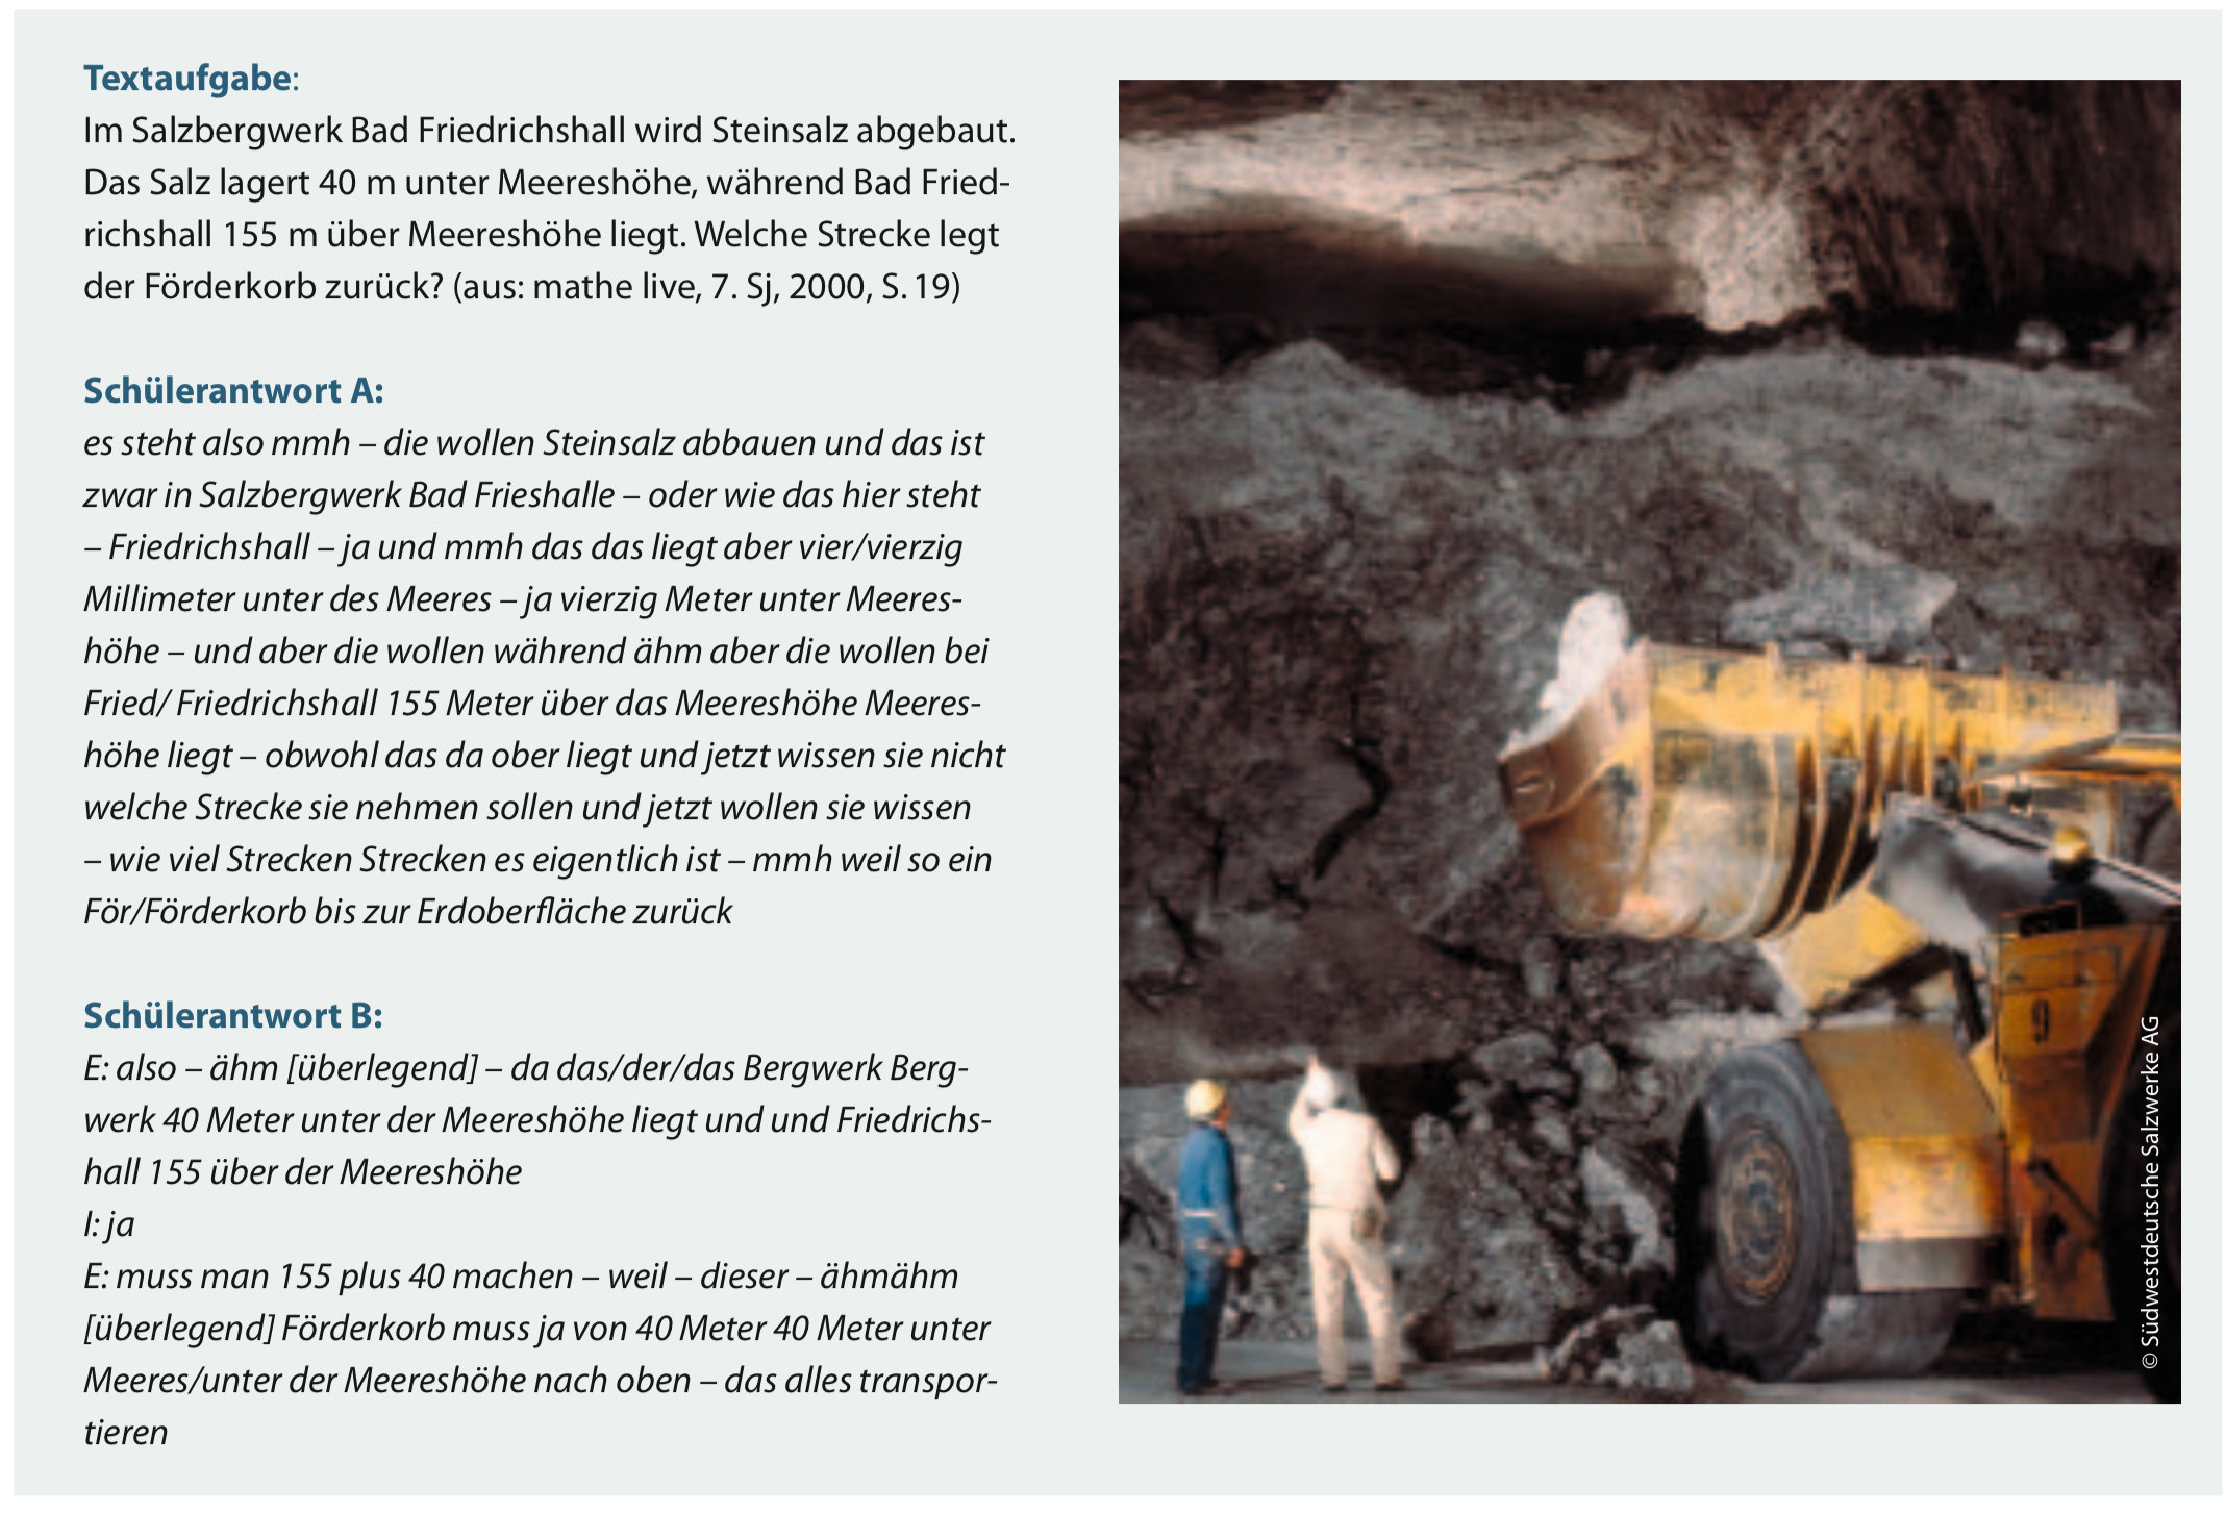
\includegraphics[height=0.68\textheight]{graphics/feilke}
\end{frame}

\begin{frame}
  {Sprachbetrachtung und Literatur im Deutsch-Abitur I}
  \pause
  Sprachlich-grammatische Betrachtung zur Literatur in Abiturarbeiten\\
  (Häcker 2009).\\[\baselineskip]
  \pause
  \centering
  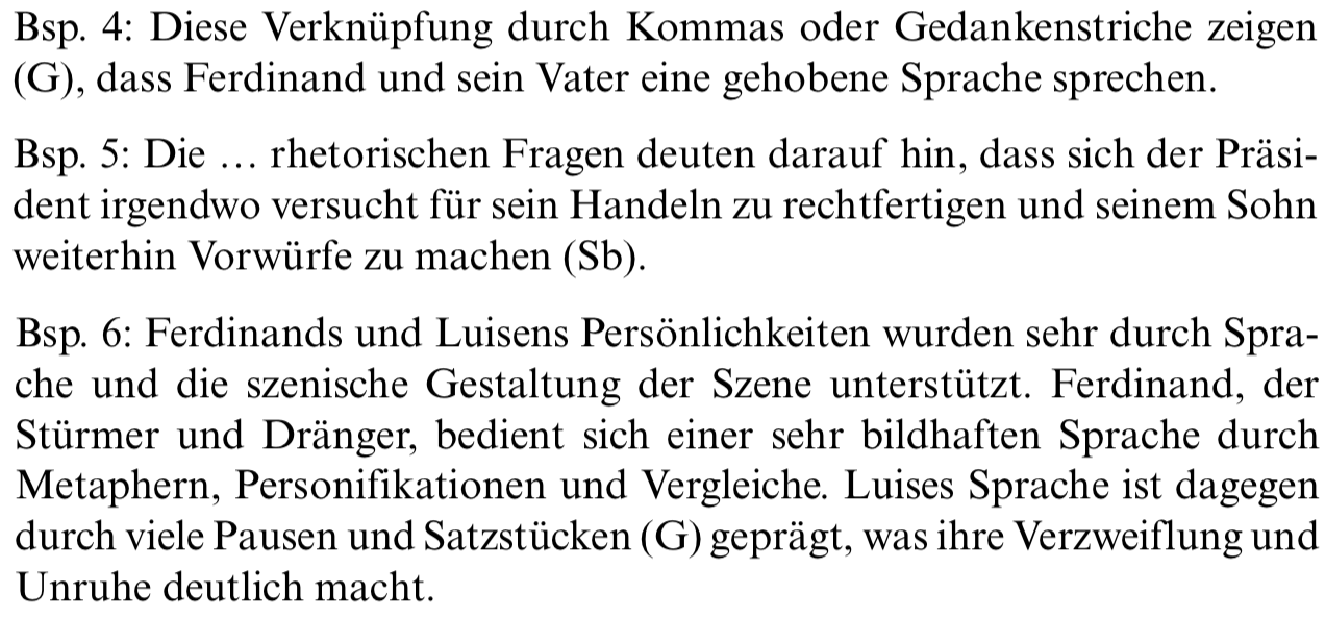
\includegraphics[height=0.5\textheight]{graphics/haecker1}
\end{frame}

\begin{frame}
  {Sprachbetrachtung und Literatur im Deutsch-Abitur II}
  Sprachlich-grammatische Betrachtung zur Literatur in Abiturarbeiten\\
  (Häcker 2009).\\[\baselineskip]
  \centering
  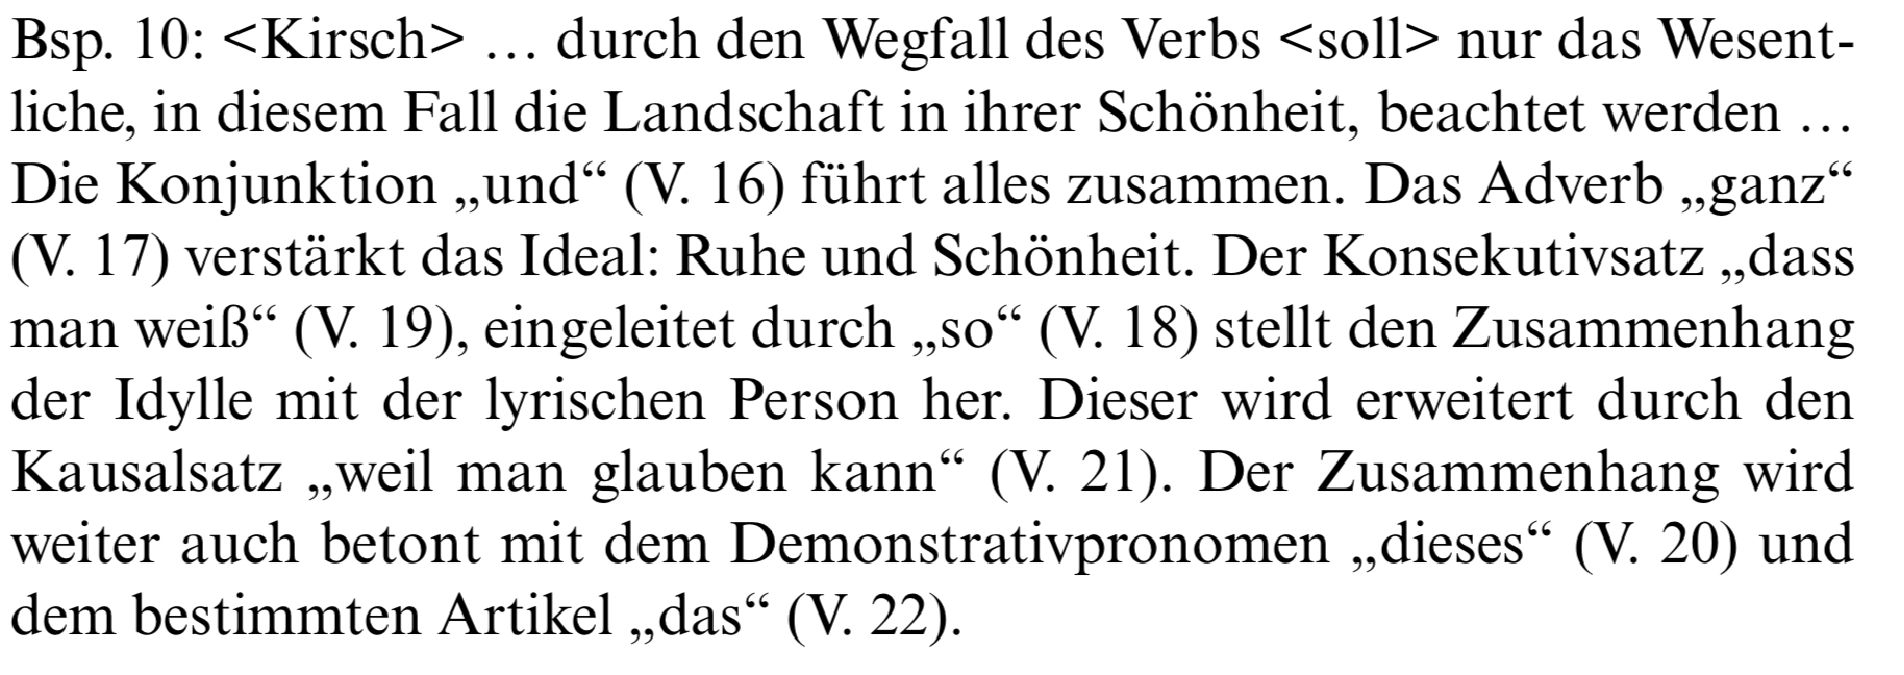
\includegraphics[height=0.4\textheight]{graphics/haecker2}
\end{frame}

\begin{frame}
  {Bildungssprache}
  \pause
  \alert{\textit{Der Deutschunterricht führt zu einem kompletten Umbau\\
  der Grammatik des Kindes.}} (nach Bredel\slash Eisenberg)\\[\baselineskip]
  \pause
  \begin{itemize}[<+->]
    \item Anforderungen:
    \begin{itemize}[<+->]
      \item Darstellung komplexer Sachverhalte
      \item \dots und nicht-faktischer (z.\,B.\ hypothetischer) Sachverhalte
      \item Intensionalität
      \item Registerbewusstsein
    \end{itemize}
        \vspace{\baselineskip}
      \item Eigenschaften:
    \begin{itemize}[<+->]
      \item dekontextualisiert
      \item schriftorientiert
      \item normorientiert
    \end{itemize}
        \vspace{\baselineskip}
      \item \alert{Das alles ist verknüpft mit spezifischen grammatischen Formen!}
  \end{itemize}
\end{frame}

\begin{frame}
  {Sprachbetrachtung}
  \pause
  \begin{itemize}[<+->]
    \item Bildungssprache $\Leftrightarrow$ Sprachbetrachtung
      \vspace{\baselineskip}
    \item Bewusstsein über richtige und angemessene Form
      \vspace{\baselineskip}
    \item explizite Sprachbetrachtung im Alltag:
      \begin{itemize}[<+->]
        \item Selbst- oder Fremdkorrektur
        \item Suche nach dem richtigen Ausdruck
        \item Orthographie optimieren
        \item Texte optimieren
        \item Begriffe definieren
        \item Grammatikalität beurteilen
      \end{itemize}
  \end{itemize}
\end{frame}

\begin{frame}
  {Die Ausgangsbasis: vorliterate Kinder und Sprachbetrachtung}
  \pause
  Klassische Studien nach Bredel (2013), Bredel et al. (2017) (s.\ EGBD3: 57--58)\\
  (Beispiele hier vereinfacht\slash dem Effekt nach neu konstruiert)\\[\baselineskip]
  \pause
  \begin{itemize}[<+->]
    \item \alert{bedeutungsbezogene} bzw.\ \alert{holistische} Betrachtung
    \item \textit{Welches Wort ist länger: Haus oder Streichholzschächtelchen?} --- \textit{Haus.}
    \item Assoziationen zu Substantiven wie \textit{Bett}: \alert{Ereignisse} \textit{schlafen gehen} usw.\\
      Erwachsene: \alert{Substantive} für andere Möbel usw.
    \item \textit{Warum heißt der Geburtstag  "`Geburtstag"'?} ---\\
      \textit{"`Weil es Geschenke und Kuchen gibt."'}
    \item \textit{Wieviele Wörter in "`Im alten Haus lebt eine junge Frau."'} --- \textit{Zwei.}
    \item \textit{Wieviele Wörter in "`Alex hat sieben Schwestern."'} --- \textit{Sieben.}
      \vspace{\baselineskip}
    \item Erfolgreich: \textit{Benenne das letzte Wort des Satzes.}
    \item[$\Rightarrow$] Die mentale Grammatik basiert auf Wörtern,\\
      der sprachbetrachtende Zugriff allerdings noch nicht!
  \end{itemize}
\end{frame}

\begin{frame}
  {Schulunterricht}
  \begin{itemize}[<+->]
    \item \alert{systematisch}
      \begin{itemize}
        \item in knapper Zeit das Ganze im Blick
      \end{itemize}
      \vspace{\baselineskip}
    \item funktional im Sinn von \alert{Form-Funktion-Beziehung}
      \begin{itemize}
        \item Formen systematisieren
        \item erst dann auf Funktionen beziehen
      \end{itemize}
      \vspace{\baselineskip}
    \item \alert{induktiv}
      \begin{itemize}
        \item keine rein deduktive Anwendung vorgegebener Begriffe
        \item Erkenntnisprozesse über sprachliche Formen und Funktionen
        \item \alert{\textit{Grammatik machen}} (Eisenberg)
      \end{itemize}
  \end{itemize}
\end{frame}

\begin{frame}
  {Aufgaben von Lehrpersonen}
  \pause
  \alert{\textit{Lehrkräften wird die Sprache der Lernenden anvertraut.}} (nach Eisenberg)\\[\baselineskip]
  \pause
  \begin{itemize}[<+->]
    \item Unterrichten der Schrift, Orthographie und Schreibung
    \item Unterweisung in Bildungssprache\slash Sprachbetrachtung
    \item Erkennen und \alert{Einordnen} von \alert{sprachlichen Defiziten}
    \item Erkennen von \alert{Interferenz mit Dialekt bzw.\ anderen Erstsprachen}
    \item \alert{Bewerten} von sprachlichen Leistungen
    \item \alert{Erklären} der Bewertung (auch gegenüber Eltern)
      \vspace{\baselineskip}
    \item[$\Rightarrow$] Anforderung: vertieftes Wissen über Sprache, vor allem Grammatik
    \item[$\Rightarrow$] Methode der sprachlichen Analyse über Faktenwissen hinaus
    \item[$\Rightarrow$] \rot{Die Grammatik für Studierende des Lehramts ist eine völlig andere\\
      als die, die sie später an Schulkinder und Jugendliche vermitteln!}
  \end{itemize}
\end{frame}

\begin{frame}
  {"`Wozu brauchen wir das denn?"'}
  \pause
  \begin{itemize}[<+->]
    \item beantwortet
    \item Linguistik und Fachdidaktik: keine praktische Anleitungen\\
      für erfolgreiche Schulstundenkonzepte
    \item Grundausbildung im \alert{Umgang mit Sprache} (Linguistik)\\
      und zum \alert{richtigen Handeln im Unterricht} (Fachdidaktik; nach Bredel)
      \vspace{\baselineskip}
    \item Minimalforderung: \alert{Examinierte Lehrkräfte müssen die\\
      Aufgaben für die späteren Lernenden selber lösen und einordnen können.}
    \item \alert{Bis nächste Woche: Bitte schauen Sie sich den Fragebogen\\
      aus Schäfer \& Sayatz (2017) an (siehe Blackboard).}
  \end{itemize}
\end{frame}


  
\section{Rückblick}

\begin{frame}
  {Erinnerung an letzte Woche: Grammatik}
  \pause
  \begin{itemize}[<+->]
    \item unbewusste Verarbeitung → Akzeptabilität
    \item Gesetzmäßigkeiten = Regularitäten
    \item \alert{System} von Gesetzmäßigkeiten
    \item \alert{definiertes} System → Grammatikalität
    \item \alert{Kern}: Klassen\slash Regularitäten mit hoher Typenfrequenz\\
      Peripherie: niedrige Typenfrequenz
    \item Norm = Beschreibung des Grundkonsenses
  \end{itemize}
\end{frame}

\begin{frame}
  {Erinnerung an letzte Woche: Didaktik}
  \pause
  \begin{itemize}[<+->]
    \item Ziel des Deutschunterrichts: \alert{Bildungssprache}
    \item Bildungssprache + Schriftlichkeit + Norm
    \item Sprachbetrachtung im Alltag
    \item Sprachbetrachtung als Lehrkonzept
    \item Unterricht: \alert{systematisch}, \alert{Form-Funktion}, \alert{induktiv}
    \vspace{\baselineskip}
  \item \rot{Die Grammatik für Studierende des Lehramts ist eine völlig andere\\
      als die, die sie später an Schulkinder und Jugendliche vermitteln!}
  \end{itemize}
\end{frame}

\begin{frame}
  {Der Fragebogen}
  \pause
  \centering
  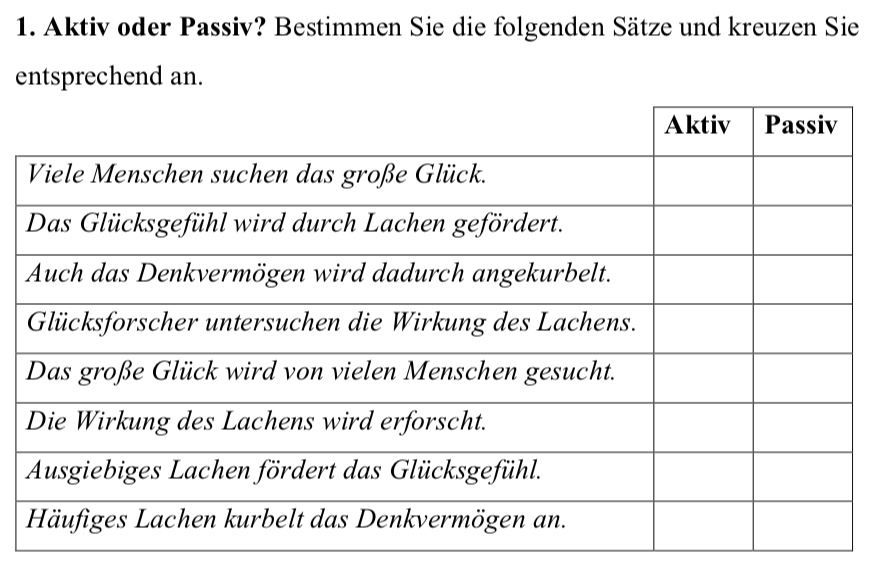
\includegraphics[width=0.75\textwidth]{\GRAPHPATH/01}
\end{frame}

\begin{frame}
  {Der Fragebogen}
  \centering
  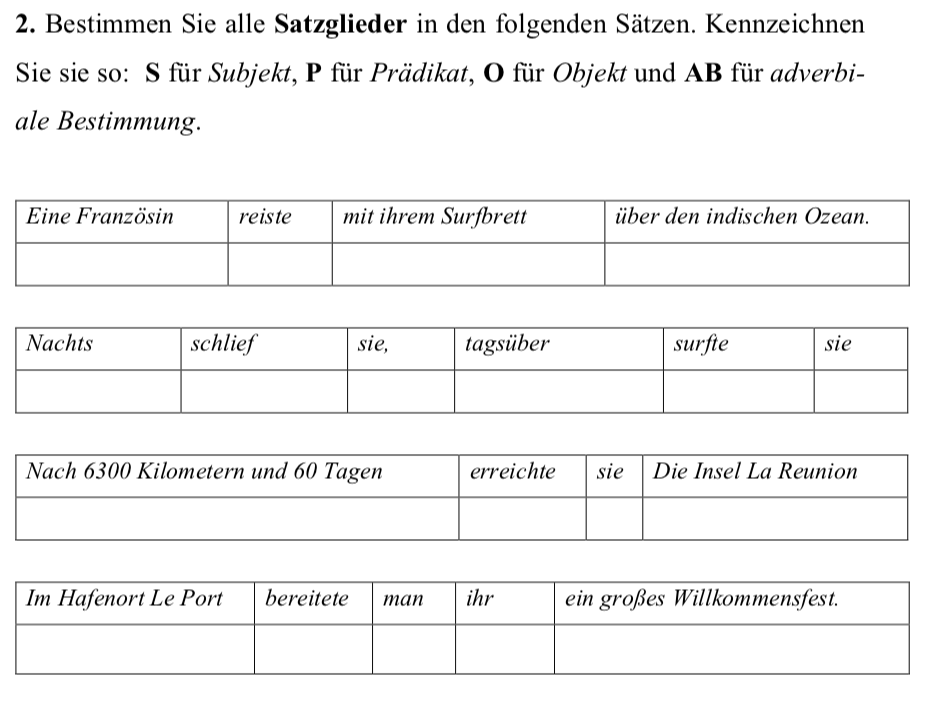
\includegraphics[width=0.75\textwidth]{\GRAPHPATH/02}
\end{frame}

\begin{frame}
  {Der Fragebogen}
  \centering
  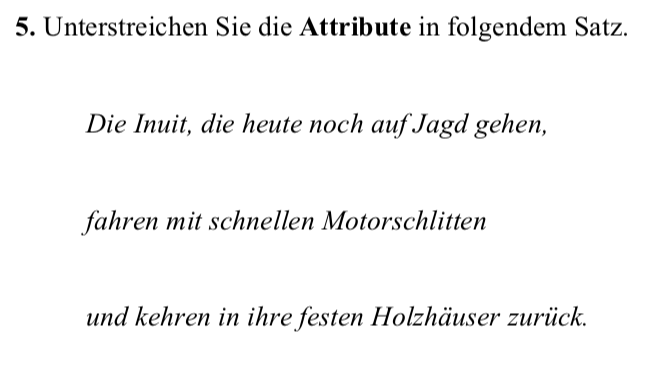
\includegraphics[width=0.75\textwidth]{\GRAPHPATH/03}
\end{frame}

\begin{frame}
  {Der Fragebogen}
  \centering
  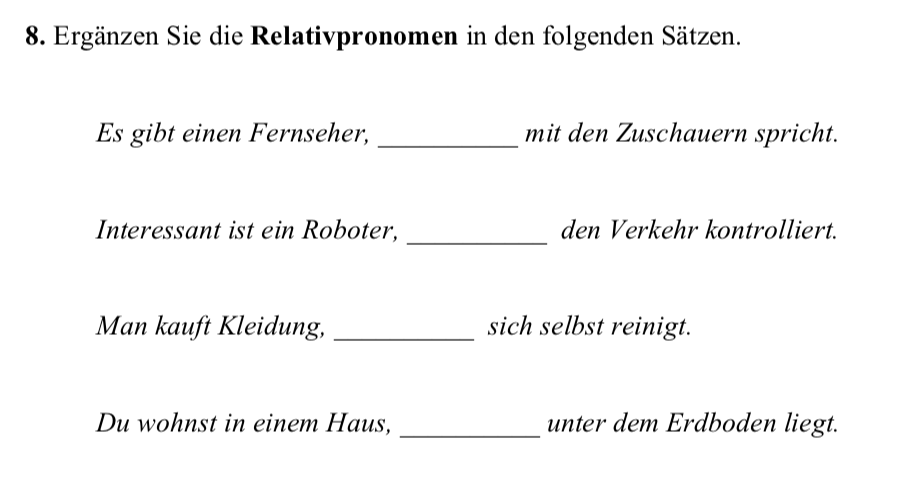
\includegraphics[width=0.75\textwidth]{\GRAPHPATH/04}
\end{frame}

\begin{frame}
  {Auswertung}
  \pause
  \centering
  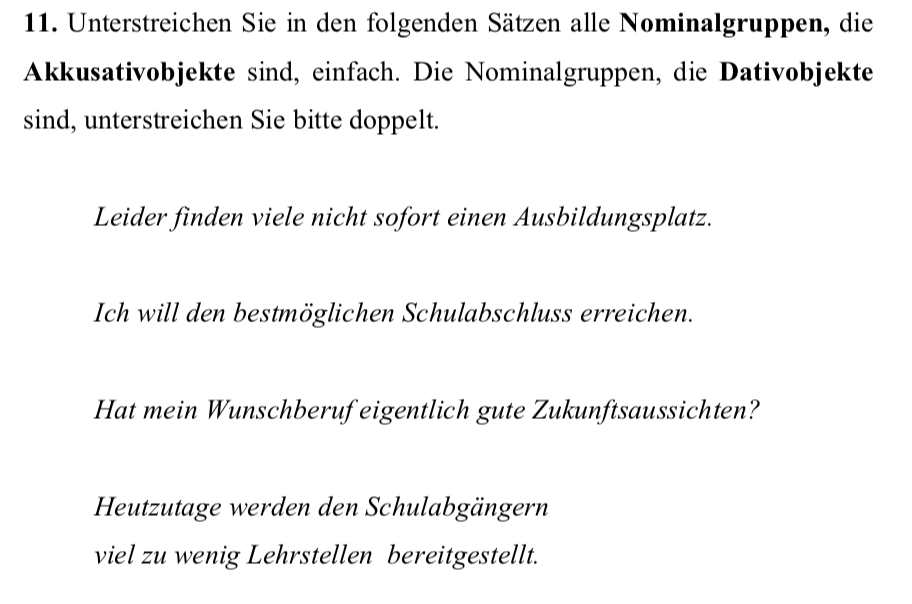
\includegraphics[width=0.75\textwidth]{\GRAPHPATH/05}
\end{frame}

\begin{frame}
  {Auswertung}
  \centering
  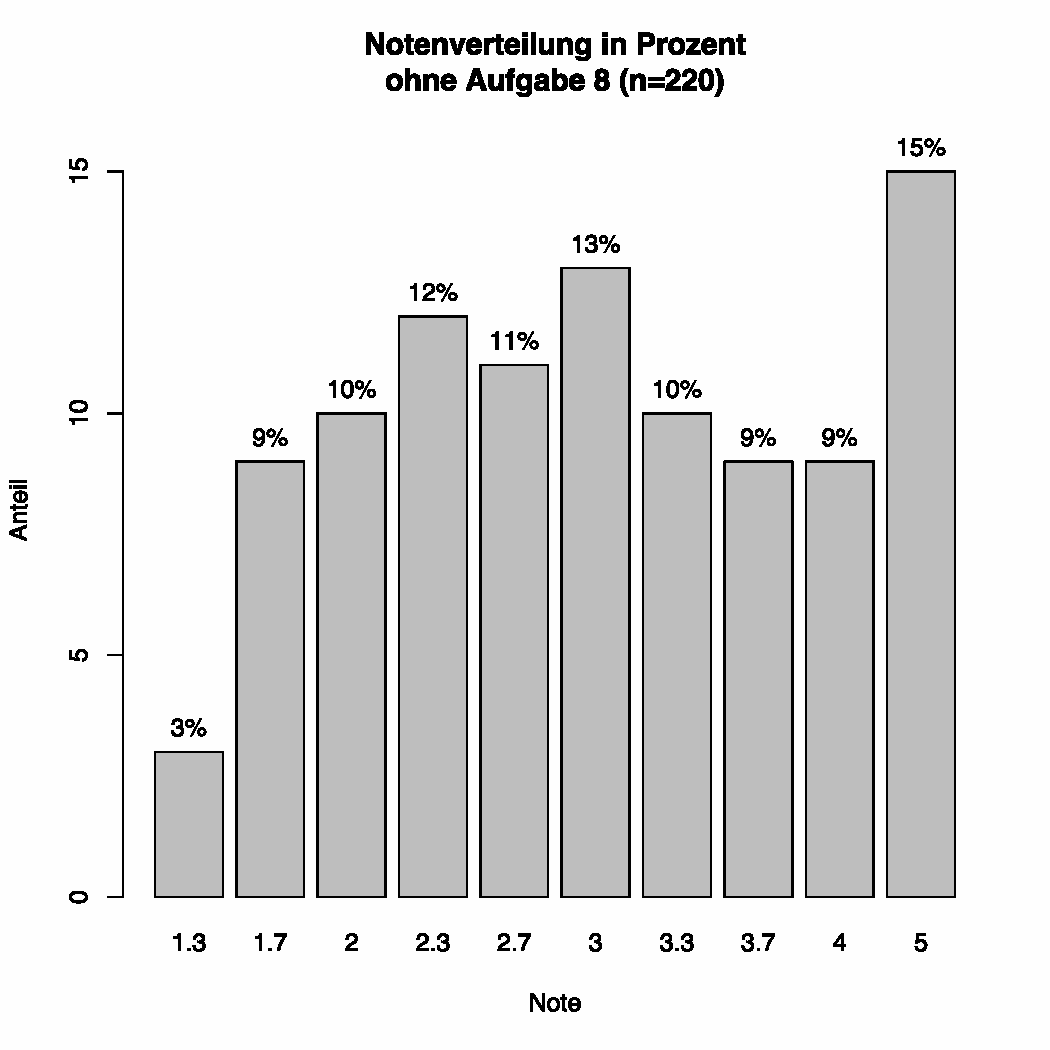
\includegraphics[width=0.6\textwidth]{\GRAPHPATH/notenspiegel}
\end{frame}

\begin{frame}
  {Auswertung}
  \centering
  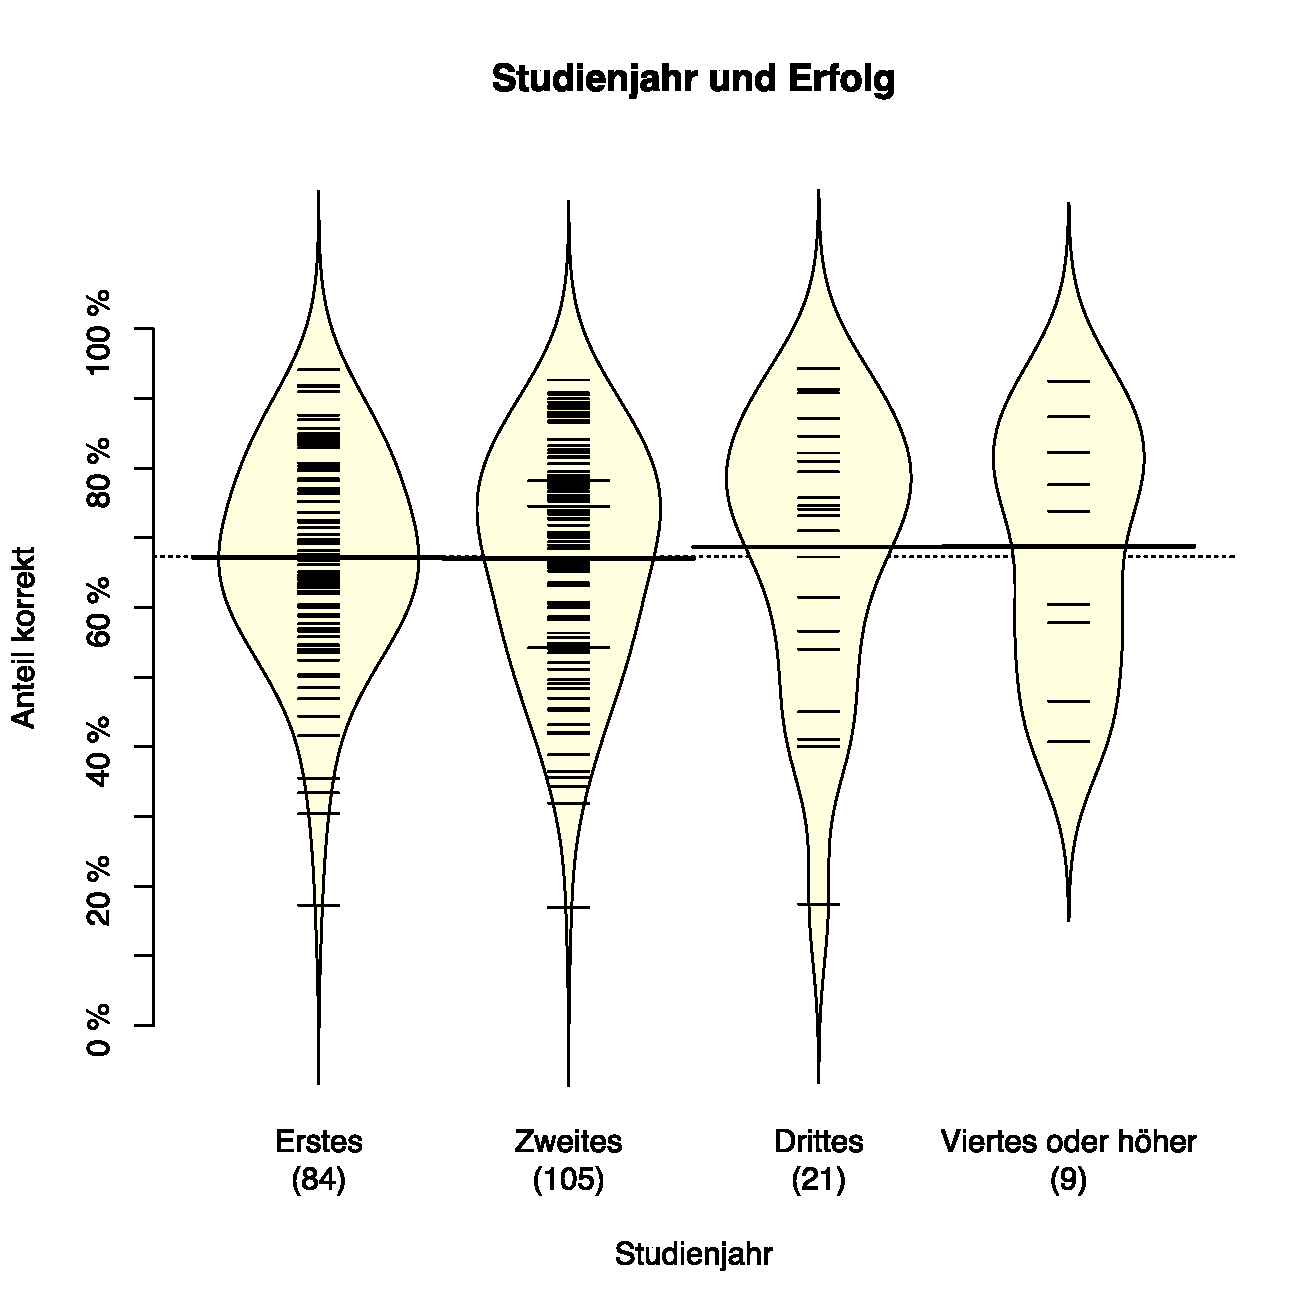
\includegraphics[width=0.6\textwidth]{\GRAPHPATH/semester}
\end{frame}

\begin{frame}
  {Auswertung}
  \centering
  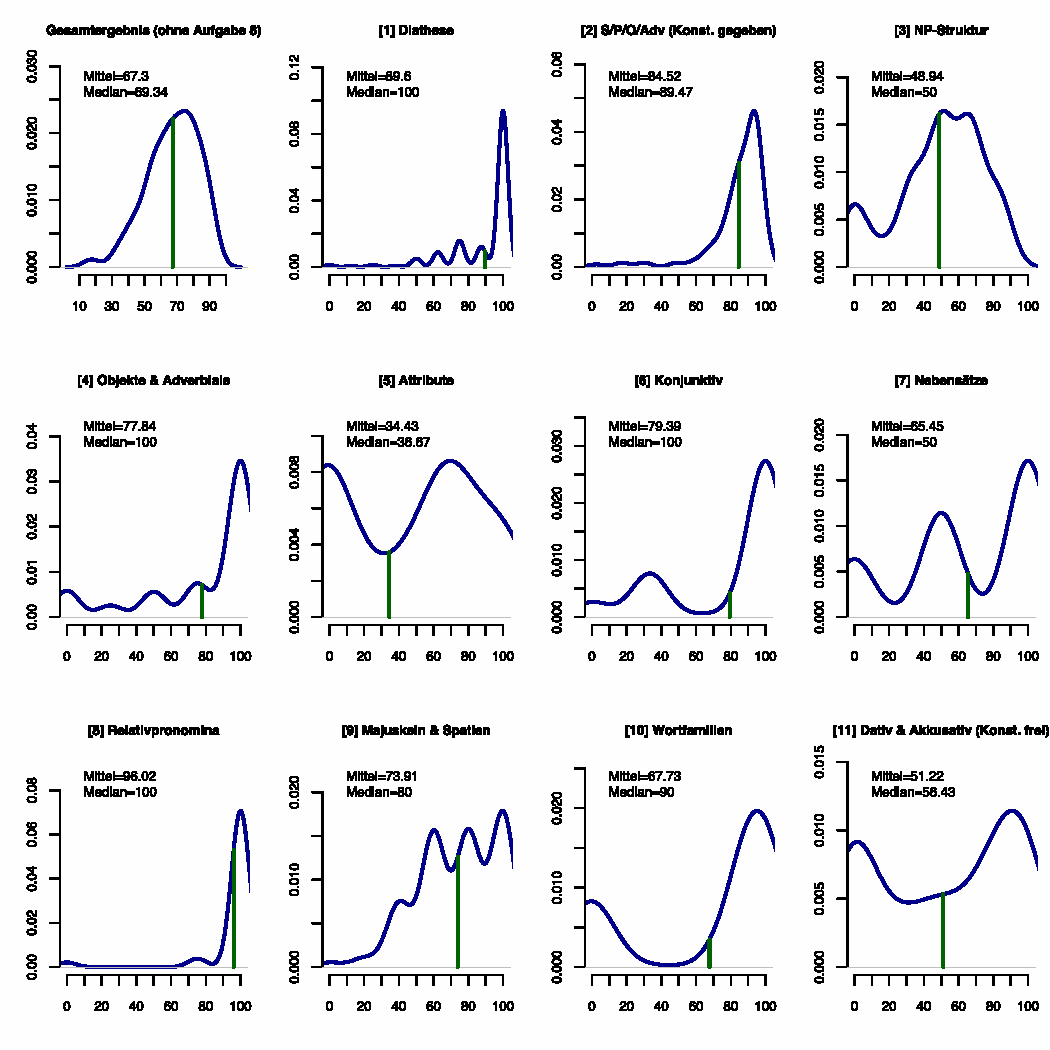
\includegraphics[width=0.6\textwidth]{\GRAPHPATH/prozentverteilung}
\end{frame}

\begin{frame}
  {Wichtige Bücher für das gesamte Studium}
  \pause
  \begin{itemize}[<+->]
    \item Grammatik\slash Linguistik:
      \begin{itemize}[<+->]
        \item \alert{\citet{Eisenberg2013a}}
        \item \alert{\citet{Eisenberg2013b}}
        \item \citet{Mueller2018} (Grammatiktheorie)
      \end{itemize}
    \vspace{\baselineskip}
    \item Linguistisch orientierte Fachdidaktik:
      \begin{itemize}[<+->]
        \item \alert{\citet{Menzel2017}}, dazu \citet{EisenbergMenzel1995}
        \item \alert{\citet{Bredel2013}}
        \item \citet{BredelEa2017} (insbesondere Grundschule)
        \item \citet{BredelPieper2015}
      \end{itemize}
  \end{itemize}
\end{frame}

\section{Phonetik}

\begin{frame}
  {Übersicht}
  \pause
  \begin{itemize}[<+->]
    \item Was ist \alert{Phonetik}?
    \item Was hat Phonetik mit \alert{Bildungssprache} zu tun?
    \item Welche \alert{Organe} sind an der Artikulation beteiligt?
    \item \alert{Wie} werden Vokale und Konsonanten artikuliert?
    \item \alert{Wo} werden Vokale und Konsonanten artikuliert?
    \item Welche Konsonanten und Vokale gibt es im \alert{Standard}?
  \end{itemize}
\end{frame}

\begin{frame}
  {Medien}
  \pause
  \begin{itemize}[<+->]
    \item akustisch
    \item artefaktisch (\zB Schrift)
    \item gestisch
    \vspace{\baselineskip}
  \item Beziehungen?
  \item \textit{Das schreibt man wie man es spricht?}
  \end{itemize}
\end{frame}

\begin{frame}
  {Methode und Ziele}
  \pause
  \begin{itemize}[<+->]
    \item \alert{artikulatorische} Phonetik: Produktion
    \item \alert{perzeptorische} Phonetik: Wahrnehmung
    \item \alert{akustische} Phonetik: physikalische Gestalt
    \vspace{\baselineskip}
  \item Warum \rot{artikulatorisch}?
    \begin{itemize}[<+->]
      \item Transkriptionsalphabete
      \item Grundlage der Phonologie
      \item Grundlage Sprecherziehung i.\,w.\,S.
      \item weitgehend apparatefrei möglich
      \item weitgehend experimentfrei möglich
    \end{itemize}
    \vspace{\baselineskip}
  \item Empfohlene Literatur: \citet{RuesEa2009}
  \end{itemize}
\end{frame}

\begin{frame}
  {Phonetik und Bildungssprache}
  \pause
  \begin{itemize}[<+->]
    \item phonetische Normbeherrschung: Primärmerkmal
    \vspace{0.5\baselineskip}
    \item Prestige
      \begin{itemize}[<+->]
        \item William Labov 1966: (nicht-)rhotische Varietäten des Englischen
        \item drei Kaufhäuser in NYC, drei "`Schichten"'
        \item \textit{r} nach Vokal als \alert{Schichtindikator}
        \item situative Anpassung
      \end{itemize}
  \item Anke Engelkes \textit{Deutschkurs für türkische Mitbürger*innen}
    \vspace{0.5\baselineskip}
    \item \alert{Dialekte, Soziolekte, Kiezsprachen erhalten!}
    \item \rot{Standard lehren!}
    \item zukünftige Lehrpersonen
      \begin{itemize}
        \item Phonetik $\not\subset$ Schulstoff
        \item \rot{Erkennen von Ausspracheproblemen in der Norm}
        \item \alert{richtige Reaktion nur mit phonetischem Wissen}
      \end{itemize}
  \end{itemize}
\end{frame}

\begin{frame}
  {Artikulationsorgane}
  \pause
  \centering
  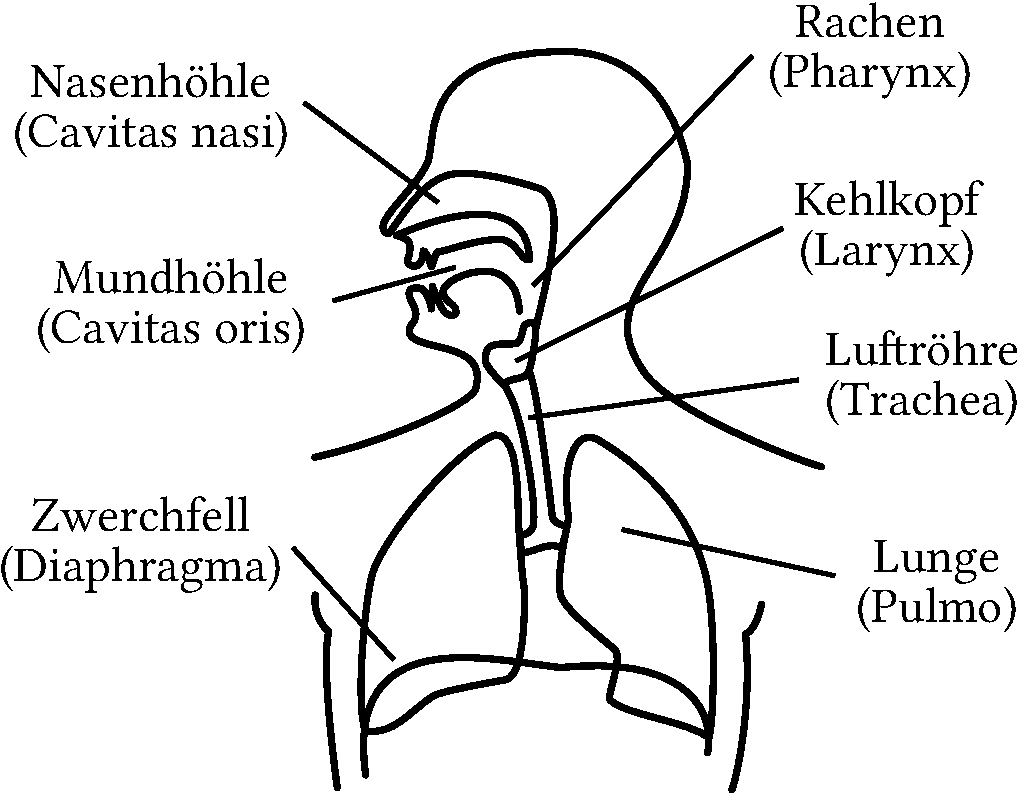
\includegraphics[height=0.7\textheight]{\GRAPHPATH/ueberblick}
\end{frame}

\begin{frame}
  {Mundraum}
  \pause
  \centering
  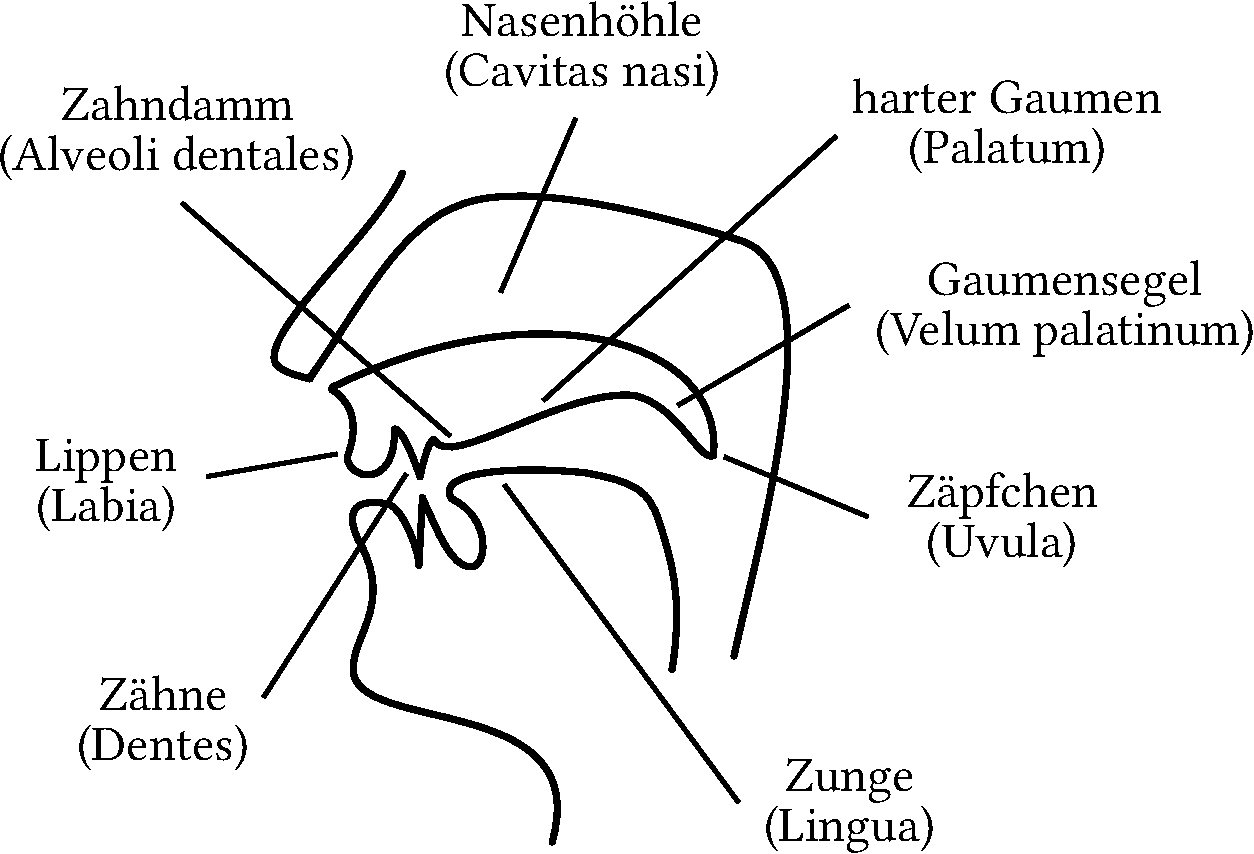
\includegraphics[height=0.7\textheight]{\GRAPHPATH/mundraum}
\end{frame}

\begin{frame}
  {Artikulationen: Konsonanten}
  \pause
    \begin{exe}
      \ex \alert{P}ole, \alert{B}ohle; \alert{T}ank, \alert{D}ank; \alert{g}ilt, \alert{k}illt
      \pause
      \ex \alert{F}ee, \alert{w}eh; hei\alert{ß}er, hei\alert{s}er; schli\alert{ch}, \alert{J}ubel; Ba\alert{ch}, \alert{R}une
      \pause
      \ex \alert{Pf}anne; \alert{Z}irkus; Ma\alert{tsch}
      \pause
      \ex \alert{M}us; \alert{N}uss; Go\alert{ng}
    \end{exe}
    \pause
    \Large
    \begin{itemize}
      \item \alert{Stimmhaftigkeit}
    \end{itemize}
\end{frame}


\begin{frame}
  {Artikulationen: Konsonanten}
  \pause
  \begin{exe}
    \ex \alert{P}a\alert{pp}e, \alert{b}e\alert{b}auen
    \pause
    \ex \alert{T}in\alert{t}e, \alert{d}ul\alert{d}en
    \pause
    \ex \alert{K}na\alert{ck}, \alert{g}e\alert{g}en
    \pause
    \ex Cha\alert{?}ot (Chaos)
    \ex \alert{?}Anfang, \alert{?}über, \alert{?}ohne, \alert{?}Uhr, \dots
  \end{exe}
    \pause
    \Large
    \begin{itemize}
      \item \alert{Plosive}
    \end{itemize}
\end{frame}


\begin{frame}
  {Artikulationen: Konsonanten}
  \pause
  \begin{exe}
    \ex \alert{f}ün\alert{f}, \alert{w}ehe
    \pause
    \ex Bu\alert{s}, \alert{S}ahne
    \pause
    \ex Bä\alert{ch}e, \alert{J}och
    \pause
    \ex Ba\alert{ch}e, \alert{R}asen
  \end{exe}
    \pause
    \Large
    \begin{itemize}
      \item \alert{Frikative}
    \end{itemize}
\end{frame}

\begin{frame}
  {Artikulationen: Konsonanten}
  \pause
  \begin{exe}
    \ex \alert{Pf}anne, To\alert{pf} 
    \pause
    \ex \alert{Z}ange, Schli\alert{tz}
    \pause
    \ex Ma\alert{tsch} (\alert{Ch}ips)
    \pause
    \ex (\alert{Dsch}ungel)
  \end{exe}
    \pause
    \Large
    \begin{itemize}
      \item \alert{Affrikaten}
    \end{itemize}
\end{frame}

\begin{frame}
  {Artikulationen: Konsonanten}
  \pause
  \begin{exe}
    \ex \alert{L}icht, Ba\alert{ll}
  \end{exe}
    \pause
    \Large
    \begin{itemize}
      \item \alert{Approximanten}
    \end{itemize}
    \Zeile
  \pause
  \begin{exe}
    \ex \alert{M}aus, Bau\alert{m}
    \pause
    \ex \alert{N}ase, Ki\alert{nn}
    \pause
    \ex Ri\alert{ng}
  \end{exe}
    \pause
    \Large
    \begin{itemize}
      \item \alert{Nasale}
    \end{itemize}
\end{frame}


\begin{frame}
  {Artikulationen: Vokale}
  \pause
  \begin{exe}
    \ex T\alert{ie}r, T\alert{ü}r; g\alert{u}t
    \pause
    \ex w\alert{e}nig, Fl\alert{ö}te; H\alert{o}se
    \pause
    \ex k\alert{ä}me
    \pause
    \ex B\alert{a}d
    \Zeile
    \pause
    \ex K\alert{i}nd, M\alert{ü}ndel; B\alert{u}s
    \pause
    \ex k\alert{ä}mme, k\alert{ö}nnen; Sch\alert{o}ck
    \pause
    \ex T\alert{a}nne
    \Zeile
    \pause
    \ex s\alert{ei}, Pf\alert{au}, H\alert{eu}
    \Zeile
    \pause
    \ex Tüt\alert{e}, b\alert{e}sonders, Eh\alert{e}, \dots
  \end{exe}
\end{frame}


\begin{frame}
  {Artikulationsarten}
  \pause
  \resizebox{\textwidth}{!}{
  \begin{tikzpicture}[every text node part/.style={align=center}]
    \node (UeVok) at (0,0)  {\textbf{Vokale}\\(prototypisch\\silbisch)};
    \node (UeApr) at (2.5,2)  {Approximanten};
    \node (UeNas) at (5,2)  {Nasale};
    \node (UeFri) at (7.5,2)  {Frikative};
    \node (UeAfr) at (10,2) {Affrikaten};
    \node (UePlo) at (12.5,2)  {Plosive};

    \node (UeSon) at (0,4) {\textbf{Sonoranten}\\(Klanglaute)};
    \node (UeObs) at (12.5,4) {\textbf{Obstruenten}\\(Geräuschlaute)};

    \node (UeKon) at (12.5,0) {\textbf{Konsonanten}\\(prototypisch\\nicht silbisch)};

    \draw (UeSon) to (UeVok);
    \draw [bend left] (UeSon) to (UeApr);
    \draw [bend left] (UeSon) to (UeNas);

    \draw (UeObs) to (UePlo);
    \draw [bend right] (UeObs) to (UeFri);
    \draw [bend right] (UeObs) to (UeAfr);

    \draw [bend right] (UeApr) to (UeKon);
    \draw [bend right] (UeNas) to (UeKon);
    \draw (UePlo) to (UeKon);
    \draw [bend right] (UeFri) to (UeKon);
    \draw [bend right] (UeAfr) to (UeKon);
  \end{tikzpicture}}
\end{frame}

\begin{frame}
  {Artikulationsorte (Konsonanten)}
  \pause
  \begin{exe}
    \ex \alert{P}a\alert{pp}e, \alert{B}irne, \alert{M}ulch
    \pause
    \ex \alert{F}ahne, \alert{W}itz, \alert{Pf}usch
    \pause
    \ex \alert{T}raum, \alert{d}ort, Mi\alert{s}t, \alert{s}ing, \alert{Z}under, \alert{L}uft, \alert{n}och
    \pause
    \ex Bu\alert{sch}, \alert{Tsch}echisch
    \pause
    \ex schle\alert{ch}t, \alert{J}unge
    \pause
    \ex Ro\alert{ck}, \alert{G}abe, Kli\alert{ng}e
    \pause
    \ex wa\alert{ch}, \alert{r}ütteln
    \pause
    \ex \alert{?}offen, \alert{h}och
  \end{exe}
\end{frame}


\begin{frame}
  {Welche Konsonanten gibt es?}
  \centering
  \resizebox{0.7\textwidth}{!}{
  \begin{tabular}{rccccccccc}
    \toprule
    \multicolumn{1}{c}{} & \Sw{\textbf{bilabial}} & \Sw{\textbf{labiodental}} & \Sw{\textbf{alveolar}} & \Sw{\textbf{palatoalveolar}} & \Sw{\textbf{palatal}} & \Sw{\textbf{velar}} & \Sw{\textbf{uvular}} & \Sw{\textbf{laryngal}} \\
    \midrule
    \textbf{stl.\ Plosiv} & p &  & t &  &  & k &  & ʔ \\
    \textbf{sth.\ Plosiv} & b &  & d &  &  & g &  &  \\
    \textbf{stl.\ Frikativ} &  & f & s & ʃ & ç &  & χ & h \\
    \textbf{sth.\ Frikativ} &  & v & z &  & ʝ &  & ʁ &  \\
    \textbf{stl.\ Affrikate} &  & p͡f & t͡s & t͡ʃ &  &  &  &  \\
    \textbf{lateraler Approximant} &  &  & l &  &  &  &  &  \\
    \textbf{Nasal} & m &  & n &  &  & ŋ &  &  \\
    \bottomrule
  \end{tabular}  
  }
\end{frame}


\begin{frame}[fragile]
  {Welche Vokale gibt es?}
  \begin{center}
  \resizebox{0.6\textwidth}{!}{
  \begin{tikzpicture}[scale=2.5,baseline=default]
    \large
    \tikzset{
      vowel/.style={fill=white, anchor=mid, text depth=0ex, text height=1ex},
      dot/.style={circle,fill=black,minimum size=0.4ex,inner sep=0pt,outer sep=-1pt},
    }

    \coordinate (hf) at (0,2); % high front
    \coordinate (hb) at (2,2); % high back
    \coordinate (lf) at (1,0); % low front
    \coordinate (lb) at (2,0); % low back
    \def\V(#1,#2){barycentric cs:hf={(3-#1)*(2-#2)},hb={(3-#1)*#2},lf={#1*(2-#2)},lb={#1*#2}}

    % Chart key (vorne -- hinten).
    \draw [{Latex[round]}-] (\V (-.25,0))   -- (\V (-.25,.5)) node [above left] {\footnotesize vorne};
    \draw [-{Latex[round]}] (\V (-.25,1.5)) -- (\V (-.25,2))  node [above left] {\footnotesize hinten};
    \path (\V (-.25,1)) node[above] {\footnotesize zentral};

    % Chart key (hoch--tief).
    \draw [{Latex[round]}-] (\V (0,-.25)) -- +(270:.5cm)  node [above right,rotate=90] (vokaltrapez1) {\footnotesize hoch};
    \draw [{Latex[round]}-] (\V (3,-2.5)) -- +(270:-.5cm) node [above left,rotate=90] (vokaltrapez2) {\footnotesize tief};
    \path (\V (1.5,-1)) node[above,rotate=90] {\footnotesize mittel};

    % Grid. 
    \draw [gray, thick] (\V(0,0)) -- (\V(0,2));
    \draw [gray, thick] (\V(1,0)) -- (\V(1,2));
    \draw [gray, thick] (\V(2,0)) -- (\V(2,2));
    \draw [gray, thick] (\V(3,0)) -- (\V(3,2));
    \draw [gray, thick] (\V(0,0)) -- (\V(3,0));
    \draw [gray, thick] (\V(0,1)) -- (\V(3,1));
    \draw [gray, thick] (\V(0,2)) -- (\V(3,2));

    % Unrounded-rounded pairs.
    \path (\V(0,0))     node[vowel, left]     {i} node[vowel, right] (y) {y} node[dot] {};
    \path (\V(0.5,0.5)) node[vowel, left]     {ɪ} node[vowel, right] (Y) {ʏ} node[dot] {};
    \path (\V(1,0))     node[vowel, left]     {e} node[vowel, right] (e) {ø} node[dot] {};
    \path (\V(2,0))     node[vowel, left] (E) {ɛ} node[vowel, right] (ee) {œ} node[dot] {};

    % Unpaired symbols.
    \path (\V(1.5,1))    node [vowel] (schwa)  {ə};
    \path (\V(2.5,1))    node [vowel] (schwaa) {ɐ};
    \path (\V(3,1))      node [vowel] (a)      {a};
    \path (\V (2,2))     node [vowel] (oo)     {ɔ};
    \path (\V (1,2))     node [vowel] (o)      {o};
    \path (\V (0,2))     node [vowel] (u)      {u};
    \path (\V (0.5,1.5)) node [vowel] (uu)     {ʊ};

    \path (a)  edge [-{Latex[round]}, bend right=15] (oo);
    \path (a)  edge [-{Latex[round]}, bend left=15]  (E);
    \path (oo) edge [-{Latex[round]}, bend right=15] (ee);
  \end{tikzpicture}
  }
  \end{center}
\end{frame}

\begin{frame}
  {Artikulation anschaulich}
  \vspace{2\baselineskip}
  \centering
  \Large Artikulationsfilme\dots
\end{frame}


\begin{frame}
  {Besonderheiten: Endrand-Desonorisierung}
  \pause
  \begin{exe}
    \ex\label{ex:auslautverhaertung011}
    \begin{xlist}
      \ex{\label{ex:auslautverhaertung012} weck [vɛk]}
      \ex{\label{ex:auslautverhaertung013} Weg [veːk]}
      \ex{\label{ex:auslautverhaertung014} Weges [veːgəs]}
    \end{xlist}
  \pause
    \ex\label{ex:auslautverhaertung015}
    \begin{xlist}
      \ex{\label{ex:auslautverhaertung016} bat [baːt]}
      \ex{\label{ex:auslautverhaertung017} Bad [baːt]}
      \ex{\label{ex:auslautverhaertung018} Bades [baːdəs]}
    \end{xlist}
  \pause
    \ex\label{ex:auslautverhaertung019}
    \begin{xlist}
      \ex{\label{ex:auslautverhaertung020} Flop [flɔp]}
      \ex{\label{ex:auslautverhaertung021} Lob [loːp]}
      \ex{\label{ex:auslautverhaertung022} Lobes [loːbəs]}
    \end{xlist}
  \end{exe}
\end{frame}


\begin{frame}
  {Besonderheiten: Silbische Nasale und Liquiden}
  \pause
  \begin{exe}
    \ex\label{ex:silbischenasaleundapproximanten023}
    \begin{xlist}
      \ex{laufen [la͡ɔfn̩]~\slash~[la͡ɔfən]}
      \ex{haben [habm̩]~\slash~[habən]}
      \ex{kriegen [kʁiːgŋ̩]~\slash~[kʁiːgən]}
      \ex{rotem [ʁoːtm̩]~\slash~[ʁoːtəm]}
      \ex{Bündel [bʏndl̩]~\slash~[bʏndəl]}
    \end{xlist}
  \end{exe}
\end{frame}

\begin{frame}
  {Besonderheiten: \textit{r}-Laute}
  \pause
  \begin{exe}
    \ex\label{ex:orthographischesr030}
    \begin{xlist}
      \ex{Tier [ti͡ɐ], Tür [ty͡ɐ]}
      \ex{Kirche [kɪ͡əçə], Bürde [bʏ͡ədə]}
      \ex{nur [nu͡ɐ]}
      \ex{Bursche [bʊ͡əʃə]}
      \ex{der [de͡ɐ], Stör [ʃtø͡ɐ]}
      \ex{Chor [ko͡ɐ]}
      \ex{gern [gɛ͡ən], Börse [bœ͡əzə]}
      \ex{Korn [kɔ͡ən]}
      \ex{Bar [ba͡ə]}
      \ex{knarr [kna͡ə]}
    \end{xlist}
  \end{exe}
\end{frame}


\begin{frame}[fragile]
  {Sekundäre Diphthonge}
  \begin{center}
  \resizebox{0.6\textwidth}{!}{
  \begin{tikzpicture}[scale=3,baseline=default]
    \large
    \tikzset{
    vowel/.style={fill=white, anchor=mid, text depth=0ex, text height=1ex},
    dot/.style={circle,fill=black,minimum size=0.4ex,inner sep=0pt,outer sep=-1pt},
    }

    \coordinate (hf) at (0,2); % high front
    \coordinate (hb) at (2,2); % high back
    \coordinate (lf) at (1,0); % low front
    \coordinate (lb) at (2,0); % low back
    \def\V(#1,#2){barycentric cs:hf={(3-#1)*(2-#2)},hb={(3-#1)*#2},lf={#1*(2-#2)},lb={#1*#2}}

    % Chart key (vorne -- hinten).
    \draw [{Latex[round]}-] (\V (-.25,0)) -- (\V (-.25,.5))  node [above left] {\footnotesize vorne};
    \draw [-{Latex[round]}] (\V (-.25,1.5)) -- (\V (-.25,2)) node [above left] {\footnotesize hinten};
    \path (\V (-.25,1)) node[above] {\footnotesize zentral};

    % Chart key (hoch--tief).
    \draw [{Latex[round]}-] (\V (0,-.25)) -- +(270:.5cm)  node [above right,rotate=90] (vokaltrapez1) {\footnotesize hoch};
    \draw [{Latex[round]}-] (\V (3,-2.5)) -- +(270:-.5cm) node [above left,rotate=90] (vokaltrapez2) {\footnotesize tief};
    \path (\V (1.5,-1)) node[above,rotate=90] {\footnotesize mittel};

    % Grid.
    \draw [gray, thick] (\V(0,0)) -- (\V(0,2));
    \draw [gray, thick] (\V(1,0)) -- (\V(1,2));
    \draw [gray, thick] (\V(2,0)) -- (\V(2,2));
    \draw [gray, thick] (\V(3,0)) -- (\V(3,2));
    \draw [gray, thick] (\V(0,0)) -- (\V(3,0));
    \draw [gray, thick] (\V(0,1)) -- (\V(3,1));
    \draw [gray, thick] (\V(0,2)) -- (\V(3,2));

    % Unrounded-rounded pairs.
    \path (\V(0,0))     node[vowel, left] {i} node [vowel, right] (y)  {y} node [dot] {};
    \path (\V(0.5,0.5)) node[vowel, left] {ɪ} node [vowel, right] (Y)  {ʏ} node [dot] {};
    \path (\V(1,0))     node[vowel, left] {e} node [vowel, right] (e)  {ø} node [dot] {};
    \path (\V(2,0))     node[vowel, left] {ɛ} node [vowel, right] (ee) {œ} node [dot] {};

    % Unpaired symbols.
    \path (\V(1.5,1))    node [vowel] (schwa)  {ə};
    \path (\V(2.5,1))    node [vowel] (schwaa) {ɐ};
    \path (\V(3,1))      node [vowel] (a)      {a};
    \path (\V (2,2))     node [vowel] (oo)     {ɔ};
    \path (\V (1,2))     node [vowel] (o)      {o};
    \path (\V (0,2))     node [vowel] (u)      {u};
    \path (\V (0.5,1.5)) node [vowel] (uu)     {ʊ};

    % Connections.
    \path (y) edge  [-{Latex[round]}, bend right=3]  (schwaa);
    \path (e) edge  [-{Latex[round]}, bend right=10] (schwaa);
    \path (ee) edge [-{Latex[round]}, bend left=20]  (schwa);
    \path (a) edge  [-{Latex[round]}, bend right=40] (schwa);
    \path (oo) edge [-{Latex[round]}, bend right=20] (schwa);
    \path (o) edge  [-{Latex[round]}, bend left=15]  (schwaa);
    \path (u) edge  [-{Latex[round]}, bend left=10]  (schwaa);
    
    \draw [-{Latex[round]}]             (Y)  -- (schwa);
    \draw [-{Latex[round]}, bend right] (uu) -- (schwa);
  \end{tikzpicture}
  }
  \end{center}
\end{frame}


\section{Vorschau}

\begin{frame}
  {Von der Phonetik zur Phonologie}
  \pause
  \begin{itemize}[<+->]
    \item Wiederholung\slash Übung der Phonetik
    \item Vorkommen von Segmenten: nicht alle überall
    \item System: zugrundeliegende Segmente und Prozesse
    \item Vorgriff auf die Graphematik: Buchstaben und Segmente
      \Zeile
    \item \rot{Lesen Sie bitte: Kapitel 5, S.~111--123}
    \item \alert{Wiederholen: Kapitel 4, S.~104--108}
  \end{itemize}

  \pause
  \pause
  \pause
  \pause
  \pause
\end{frame}



  
\section{Rückblick}

\begin{frame}
  {Erinnerung an letzte Woche: Phonetik}
  \pause
  \begin{itemize}[<+->]
    \item Artikulationsorgane
    \item Konsonanten
      \begin{itemize}
        \item Stimmton
        \item Art: Plosiv, Frikativ, Affrikate, Nasal, Approximant
      \end{itemize}
    \item Vokale:
      \begin{itemize}
        \item vorne -- hinten
        \item hoch -- tief
        \item gerundet -- ungerundet
        \item lang -- kurz
        \item Diphthonge
      \end{itemize}
    \item Sonoranten und Obstruenten
    \item r-Laute und sekundäre Diphthonge
  \end{itemize}
\end{frame}


\section{Phonologie}

\begin{frame}
  {Übersicht}
  \pause
  \begin{itemize}[<+->]
    \item \alert{Segmente} als Einheiten der Phonetik\slash Phonologie
    \item nicht alle Segmente überall: \alert{Verteilungen}
    \item Endrand-Desonorisierung, r-Vokalisierung, \textit{ich}\slash\textit{ach}-Laute usw.\\
      und \alert{Ableitung} phonetischer Formen aus lexikalischen Formen
    \item längbare, betonbare und unbetonbare Vokale
      \Zeile
    \item empfohlene Literatur: \citet{Eisenberg2013a} (Grundriss: Wort)
  \end{itemize}
\end{frame}

\begin{frame}
  {Was hat Phonologie mit Bildungs- und Normsprache zu tun?}
  \pause
  \begin{itemize}[<+->]
    \item mit Bildungssprache nicht viel
    \item mit Normsprache sehr viel
      \begin{itemize}[<+->]
        \item Viele dialektale und soziolektale Einflüsse sind\\
          phonologisch statt phonetisch.
        \item Das graphematische System ist am phonologischen orientiert.
        \item Worttrennung
      \end{itemize}
  \end{itemize}
\end{frame}

\begin{frame}
  {Segmente}
  \pause
  \begin{itemize}[<+->]
    \item Transkriptionen: \textit{Tier} [ti͡ɐ], \textit{Tür} [ty͡ɐ], \textit{rotem} [ʁoːtəm],\\
      \textit{Lob} [loːp], \textit{Bades} [baːdəs], \textit{Pfanne} [p͡fanə], \textit{Osten} [ʔɔstən]
      \vspace{\baselineskip}
    \item Warum gibt es die Basiszeichen im IPA, die es gibt? (a, ə, ɪ, ʔ, p, ʁ usw.)
      \begin{itemize}
        \item \alert{artikulatorische Untrennbarkeit}
        \item \alert{kein autonomes Verhalten potentieller Teile}
      \end{itemize}
      \vspace{\baselineskip}
    \item Sind p͡f und a͡ɔ usw.\ ein oder zwei Segmente? 
      \begin{itemize}
        \item artikulatorisch trennbar
        \item autonomes Verhalten?
        \item eigentlich eine phonologische Frage → Verteilungen
      \end{itemize}
  \end{itemize}
\end{frame}

\begin{frame}
  {Verteilungen: Beispiele}
  \pause
  \begin{exe}
    \ex
      \begin{xlist}
        \ex Tod [toːt], Kot [koːt]
        \pause
        \ex Schott [ʃɔt], Schock [ʃɔk]
      \end{xlist}
        \pause
    \ex Hang [haŋ], *[ŋah]
        \pause
    \ex
      \begin{xlist}
        \ex Sog [zoːk], besingen [bəzɪŋən], *[soːk]
        \pause
        \ex fließ [fliːs], Boss [bɔs], *[fliːz]
        \pause
        \ex heißer [ha͡ɛsɐ], heiser [ha͡ɛzɐ], Base [baːzə], Basse [basə], *[bazə]
      \end{xlist}
  \end{exe}
\end{frame}


\begin{frame}
  {Verteilung: Definition}
  \pause
  \Large
  \begin{block}{Verteilung}
    Die Verteilung eines Segments ist die Menge der Umgebungen, in denen es vorkommt.
  \end{block}
  \pause
  \Zeile
  \begin{block}{Kontrast}
    Zwei phonetisch unterschiedliche Segmente bzw.\ Merkmale stehen in einem phonologischen 
  Kontrast, wenn sie eine teilweise oder vollständig übereinstimmende Verteilung haben und dadurch einen lexikalischen bzw.\ grammatischen Unterschied markieren können.
  \end{block}
\end{frame}

\begin{frame}
  {Neutralisierung: Beispiele}
  \pause
  \begin{exe}
    \ex
    \begin{xlist}
      \ex{Weg [veːk], Weges [veːgəs]}
      \pause
      \ex{Bock [bɔk], Bockes [bɔkəs]}
      \pause
    \end{xlist}
    \ex
    \begin{xlist}
      \ex{Bad [baːt], Bades [baːdəs]}
      \pause
      \ex{Blatt [blat], Blattes [blatəs]}
      \pause
    \end{xlist}
    \ex
    \begin{xlist}
      \ex{Lob [loːp], Lobes [loːbəs]}
      \pause
      \ex{Depp [dɛp], Deppen [dɛpən]}
      \pause
    \end{xlist}
    \ex
    \begin{xlist}
      \ex aktiv [ʔaktiːf], aktive [ʔaktiːvə]
      \pause
      \ex tief [tiːf], tiefe [tiːfə]
      \pause
    \end{xlist}
    \ex
    \begin{xlist}
      \ex fies [f"|iːs], fiese [f"|iːzə]
      \pause
      \ex Bus [bʊs], Busse [bʊsə]
      \pause
    \end{xlist}
  \end{exe}
\end{frame}

\begin{frame}
  {Neutralisierung: Definition}
  \pause
  \Large
  \begin{block}{Neutralisierung}
    Eine Neutralisierung ist die Aufhebung eines phonologischen Kontrasts in einer bestimmten Position.    
  \end{block}
\end{frame}

\begin{frame}
  {Das Lexikon (Kapitel 2)}
  \pause
  \large Zum Verständnis der Phonologie ist der linguistische Begriff\\
  des Lexikons eine Grundvoraussetzung.\\
  \Large
  \Zeile
  \pause
  \begin{block}{Lexikon}
    Das \alert{Lexikon} ist die Menge aller Wörter einer Sprache, definiert durch die vollständige Angabe ihrer Merkmale und deren Werte.    
  \end{block}
  \pause
  \Zeile
  \large
  In der Phonologie ist das relevante Merkmal die \alert{Kette von Segmenten}, die ein Wort eindeutig definiert und von allen anderen Wörtern unterscheidbar macht.
\end{frame}

\begin{frame}
  {Muss man ʔ lexikalisch spezifizieren?}
  \pause
  \begin{itemize}[<+->]
    \item{[ʔan], [dan], [kan], [ʁan], [van], [man], [ban]}
    \item{[ʔoːnə], [boːnə], [loːnə], [t͡soːnə], [foːnə], [moːnə], [zoːnə]}
    \item{[ʔe͡ɐt], [ve͡ɐt], [le͡ɐt], [ke͡ɐt], [te͡ɐt], [ge͡ɐt], [he͡ɐt]}
  \end{itemize}
  \Zeile
  \pause
  \begin{itemize}[<+->]
    \item{\alert{[ʔ] kommt immer am Silbenanfang,\\
      wenn sonst kein anderer Konsonant kommt.}}
    \item{[ʔ] ist artikulatorisch und perzeptorisch wenig salient.}
    \item also: nicht lexikalisch, \alert{automatisch einsetzbar}
  \end{itemize}
\end{frame}

\begin{frame}
  {Nochmal Endrand-Desonorisierung}
  \pause
  \begin{exe}
    \ex
    \begin{xlist}
      \ex{Weg [veːk], Weges [veːgəs]}
      \ex{Bock [bɔk], Bockes [bɔkəs]}
    \end{xlist}
    \ex
    \begin{xlist}
      \ex{Bad [baːt], Bades [baːdəs]}
      \ex{Blatt [blat], Blattes [blatəs]}
    \end{xlist}
    \ex
    \begin{xlist}
      \ex{Lob [loːp], Lobes [loːbəs]}
      \ex{Depp [dɛp], Deppen [dɛpən]}
    \end{xlist}
    \ex
    \begin{xlist}
      \ex aktiv [ʔaktiːf], aktive [ʔaktiːvə]
      \ex tief [tiːf], tiefe [tiːfə]
    \end{xlist}
    \ex
    \begin{xlist}
      \ex fies [f"|iːs], fiese [f"|iːzə]
      \ex Bus [bʊs], Busse [bʊsə]
    \end{xlist}
  \end{exe}
  \pause
  \Zeile
  \begin{itemize}
    \item \alert{Aus welcher Form kann man die andere jeweils "`herleiten"'?}
  \end{itemize}
\end{frame}


\begin{frame}
  {Zugrundeliegende Form und Strukturbedingung}
  \pause
  \Large
  \begin{block}{Zugrundeliegende Form}    
    Die zugrundeliegende Form (eines Wortes) ist genau die Folge von Segmenten, die im Lexikon gespeichert wird, und auf die alle zugehörigen phonetischen Formen zurückgeführt werden können.
  \end{block}
  \pause
  \Zeile
  \begin{block}{Strukturbedingungen}
    Die Formen werden ggf. an die phonologischen Strukturbedingungen (die Regularitäten der phonologischen Grammatik) angepasst.    
  \end{block}
\end{frame}

\begin{frame}
  {Architektur der Grammatik und externer Systeme}
  \pause
  \centering
  \resizebox{0.9\textwidth}{!}{
    \begin{tabular}{ccc}
      \toprule
      \multicolumn{2}{c}{\textbf{Grammatik}} & \textbf{Externe Systeme} \\
      \midrule
      \textbf{Lexikon} & \textbf{Phonologie} & \textbf{Phonetik} \\
      \midrule
      /~/& $\Rightarrow$ & [~]\\
      zugrundeliegende Form & Anpassung an Strukturbedingungen & phonetische Realisierung \\
      \bottomrule
    \end{tabular}
  }
\end{frame}

\begin{frame}
  {Also für ʔ und Endrand-Desonorisierung}
  \pause
  \begin{itemize}[<+->]
    \item ʔ
      \begin{itemize}[<+->]
        \item /an/ $\Rightarrow$ [ʔan] 
        \item /oːnə/ $\Rightarrow$ [ʔoːnə]
        \item /e͡ɐt/ $\Rightarrow$ [ʔe͡ɐt]
      \end{itemize}
      \Zeile
    \item Endrand-Desonorisierung
      \begin{itemize}[<+->]
        \item /veːg/ $\Rightarrow$ [veːk], /bɔk/ $\Rightarrow$ [bɔk]
        \item /baːd/ $\Rightarrow$ [baːt], /blat/ $\Rightarrow$ [blat]
        \item /loːb/ $\Rightarrow$ [loːp], /dɛp/ $\Rightarrow$ [dɛp]
        \item /aktiːv/ $\Rightarrow$ [ʔaktiːf], /tiːf/ $\Rightarrow$ [tiːf]
        \item /fiːz/ $\Rightarrow$ [f"|iːs], /bʊs/ $\Rightarrow$ [bʊs]
      \end{itemize}
  \end{itemize}
\end{frame}


\begin{frame}
  {Merkmale, phonetisch motiviert (Kapitel 4)}
  \pause
  \resizebox{0.9\textwidth}{!}{
  \begin{minipage}{\textwidth}
  \begin{exe}
    \ex{\label{ex:phonetischemerkmale009} \textsc{Art}: \textit{plosiv}, \textit{frikativ}, \textit{affrikate}, \textit{nasal}, \textit{approximant}, \textit{vokal}}

    \vspace{0.5\baselineskip}
    \pause

    \ex{\label{ex:phonetischemerkmale010} \textbf{Für Konsonanten:}}\\
      \textsc{Obstruent}: $+$, $-$
    \pause

    \vspace{0.5\baselineskip} 

    \ex \textbf{Für Vokale:}
    \pause
      \begin{xlist}
        \ex \textsc{Höhe}: \textit{hoch}, \textit{halbhoch}, \textit{mittel}, \textit{halbtief}, \textit{tief}
        \pause
        \ex \textsc{Lage}: \textit{vorn}, \textit{halbvorn}, \textit{zentral}, \textit{halbhinten}, \textit{hinten}
        \pause
        \ex \textsc{Rund}: $+$, $-$
        \pause
        \ex \textsc{Lang}: $+$, $-$
      \end{xlist}

    \pause
    \vspace{0.5\baselineskip}

    \ex \textbf{Für Konsonanten:}\\
        \textsc{Ort}: \textit{laryngal}, \textit{uvular}, \textit{velar}, \textit{palatal}, \textit{palatoalveolar}, \textit{alveolar}
    \pause
    \ex \textbf{Für Obstruenten:}\\
      \textsc{Stimme}: $+$, $-$
  \end{exe}
  \end{minipage}
  }
\end{frame}


\begin{frame}
  {Endrand-Desonorisierung als Strukturbedingung}
  \pause
  \Large
  Alle Segmente mit [\textsc{Obstruent}:~$+$]\\
  sind am Silbenende [\textsc{Stimme}:~$-$].
\end{frame}


\begin{frame}
  {Verteilung von [ç] und [χ]}
  \pause
  \begin{exe}
    \ex
    \begin{xlist}
      \ex krieche, schlich, Bücher, Küche, Recht, Köche
      \pause
      \ex Tuch, Geruch, hoch, Koch, Schmach, Bach
    \end{xlist}
  \end{exe}
  \pause
  \Zeile
  \Large
  [ç] kann nicht nach Vokalen stehen, die nicht\\
  {[\textsc{Lage}: \textit{vorne}]} sind. Zugrundeliegendes /ç/\\
  wird daher nach zentralen und hinteren Vokalen\\
  weiter hinten artikuliert, nämlich als [χ].
\end{frame}

\begin{frame}
  {r-Vokalisierung}
  \pause
  \begin{exe}
    \ex
    \begin{xlist}
      \ex \textit{kleiner} [kla͡ɛ.nɐ], \textit{kleinere} [kla͡ɛ.nə.ʁə]
      \pause
      \ex \textit{Bär} [bɛ͡ɐ], \textit{Bären} [bɛː.ʁən]
      \pause
      \ex \textit{knarr} [kna͡ə], \textit{knarre} [kna.ʁə]
    \end{xlist}
  \end{exe}
  \pause
  \Zeile
  \Large
  Zugrundeliegendes /ʁ/ kann nicht am Silbenende\\
  stehen. Es wird in dieser Position als\\
  Schwa-Segment im sekundären Diphthong\\
  realisiert. Nach gespanntem Vokal folgt [ɐ],\\
  nach ungespanntem folgt [ə]. Schwa und /ʁ/\\
  werden zusammen durch [ɐ] substituiert.\\[0.5\baselineskip]
  \pause
  \alert{Gespannt?}
\end{frame}


\begin{frame}[fragile]
  {Erinnerung an die Vokale des Deutschen}
  \begin{center}
  \resizebox{0.6\textwidth}{!}{
  \begin{tikzpicture}[scale=2.5,baseline=default]
    \large
    \tikzset{
      vowel/.style={fill=white, anchor=mid, text depth=0ex, text height=1ex},
      dot/.style={circle,fill=black,minimum size=0.4ex,inner sep=0pt,outer sep=-1pt},
    }

    \coordinate (hf) at (0,2); % high front
    \coordinate (hb) at (2,2); % high back
    \coordinate (lf) at (1,0); % low front
    \coordinate (lb) at (2,0); % low back
    \def\V(#1,#2){barycentric cs:hf={(3-#1)*(2-#2)},hb={(3-#1)*#2},lf={#1*(2-#2)},lb={#1*#2}}

    % Chart key (vorne -- hinten).
    \draw [{Latex[round]}-] (\V (-.25,0))   -- (\V (-.25,.5)) node [above left] {\footnotesize vorne};
    \draw [-{Latex[round]}] (\V (-.25,1.5)) -- (\V (-.25,2))  node [above left] {\footnotesize hinten};
    \path (\V (-.25,1)) node[above] {\footnotesize zentral};

    % Chart key (hoch--tief).
    \draw [{Latex[round]}-] (\V (0,-.25)) -- +(270:.5cm)  node [above right,rotate=90] (vokaltrapez1) {\footnotesize hoch};
    \draw [{Latex[round]}-] (\V (3,-2.5)) -- +(270:-.5cm) node [above left,rotate=90] (vokaltrapez2) {\footnotesize tief};
    \path (\V (1.5,-1)) node[above,rotate=90] {\footnotesize mittel};

    % Grid. 
    \draw [gray, thick] (\V(0,0)) -- (\V(0,2));
    \draw [gray, thick] (\V(1,0)) -- (\V(1,2));
    \draw [gray, thick] (\V(2,0)) -- (\V(2,2));
    \draw [gray, thick] (\V(3,0)) -- (\V(3,2));
    \draw [gray, thick] (\V(0,0)) -- (\V(3,0));
    \draw [gray, thick] (\V(0,1)) -- (\V(3,1));
    \draw [gray, thick] (\V(0,2)) -- (\V(3,2));

    % Unrounded-rounded pairs.
    \path (\V(0,0))     node[vowel, left]     {i} node[vowel, right] (y) {y} node[dot] {};
    \path (\V(0.5,0.5)) node[vowel, left]     {ɪ} node[vowel, right] (Y) {ʏ} node[dot] {};
    \path (\V(1,0))     node[vowel, left]     {e} node[vowel, right] (e) {ø} node[dot] {};
    \path (\V(2,0))     node[vowel, left] (E) {ɛ} node[vowel, right] (ee) {œ} node[dot] {};

    % Unpaired symbols.
    \path (\V(1.5,1))    node [vowel] (schwa)  {ə};
    \path (\V(2.5,1))    node [vowel] (schwaa) {ɐ};
    \path (\V(3,1))      node [vowel] (a)      {a};
    \path (\V (2,2))     node [vowel] (oo)     {ɔ};
    \path (\V (1,2))     node [vowel] (o)      {o};
    \path (\V (0,2))     node [vowel] (u)      {u};
    \path (\V (0.5,1.5)) node [vowel] (uu)     {ʊ};

  \end{tikzpicture}
  }
  \end{center}
\end{frame}


\begin{frame}
  {Länge und Betonung und Vokalqualität im Systemkern}
  \pause
  \centering
  \begin{tabular}{cllp{0.25cm}cll}
    \toprule
    \textbf{gespannt} & \textbf{Beispiel} & \textbf{IPA} & & \textbf{ungespannt} & \textbf{Beispiel} & \textbf{IPA} \\
    \midrule
    i  & \textit{bieten} & biːtən && ɪ & \textit{bitten}  & bɪtən   \\
    y  & \textit{fühlt}  & fyːlt  && ʏ & \textit{füllt}   & fʏlt    \\
    u  & \textit{Mus}    & muːs   && ʊ & \textit{muss}    & mʊs     \\
    e  & \textit{Kehle}  & keːlə  && ɛ & \textit{Kelle}   & kɛlə    \\
    ɛ  & \textit{stähle} & ʃtɛːlə && ɛ & \textit{Ställe}  & ʃtɛlə   \\
    ø  & \textit{Höhle}  & høːlə  && œ & \textit{Hölle}   & hœlə \\
    o  & \textit{Ofen}   & ʔoːfən && ɔ & \textit{offen}   & ʔɔfən   \\
    a  & \textit{Wahn}   & vaːn   && a & \textit{wann}    & van     \\
    \bottomrule
  \end{tabular}\\
  \pause
  \Zeile
  \begin{itemize}[<+->]
    \item Laut\rot{e}, b\rot{e}schreib\rot{e}n, \dots
    \item L\rot{i}thografie, H\rot{y}draulik, B\rot{u}tan, Ph\rot{e}nol, \rot{Ö}nologie, Mes\rot{o}zoon, \dots
  \end{itemize}
\end{frame}

\begin{frame}
  {Gespanntheit im Kernwortschatz}
  \pause
  \Large
  \rot{Im Kernwortschatz sind gespannte Vokale immer\\
  betont und lang.} Zu jedem gespannten Vokal gibt es\\
  einen entsprechenden ungespannten Vokal.\\
  Der ungespannte ist betont oder unbetont,\\
  aber immer kurz.\\
  \Zeile
  \pause
  Die Länge muss also nicht markiert werden, sondern folgt\\
  aus Betonung und Gespanntheit.
\end{frame}

\begin{frame}[fragile]
  {Gespanntheit}
  \pause
  \begin{center}
    \resizebox{0.6\textwidth}{!}{
      \begin{tikzpicture}[scale=3.5,baseline=default]
        \large
        \tikzset{
        vowel/.style={fill=white, anchor=mid, text depth=0ex, text height=1ex},
        vowelgespannt/.style={circle,fill=gray!30, anchor=mid, text depth=0ex, text height=1ex,minimum size=4ex},
        dot/.style={circle,fill=black,minimum size=0.4ex,inner sep=0pt,outer sep=-1pt},
        }

        \coordinate (hf) at (0,2); % high front
        \coordinate (hb) at (2,2); % high back
        \coordinate (lf) at (1,0); % low front
        \coordinate (lb) at (2,0); % low back
        \def\V(#1,#2){barycentric cs:hf={(3-#1)*(2-#2)},hb={(3-#1)*#2},lf={#1*(2-#2)},lb={#1*#2}}

        % Chart key (vorne -- hinten).
        \draw [{Latex[round]}-] (\V (-.25,0)) -- (\V (-.25,.5))  node [above left] {\footnotesize vorne};
        \draw [-{Latex[round]}] (\V (-.25,1.5)) -- (\V (-.25,2)) node [above left] {\footnotesize hinten};
        \path (\V (-.25,1)) node[above] {\footnotesize zentral};

        % Chart key (hoch--tief).
        \draw [{Latex[round]}-] (\V (0,-.25)) -- +(270:.5cm)  node [above right,rotate=90] (vokaltrapez1) {\footnotesize hoch};
        \draw [{Latex[round]}-] (\V (3,-2.5)) -- +(270:-.5cm) node [above left,rotate=90] (vokaltrapez2) {\footnotesize tief};
        \path (\V (1.5,-1)) node[above,rotate=90] {\footnotesize mittel};

        % Grid.
        \draw [gray,thick] (\V(0,0)) -- (\V(0,2));
        \draw [gray,thick] (\V(3,0)) -- (\V(3,2));
        \draw [gray,thick] (\V(0,0)) -- (\V(3,0));
        \draw [gray,thick] (\V(0,2)) -- (\V(3,2));

        \path (\V(0,0))      node[vowelgespannt] (i)   {i};
        \path (\V(0.25,0))   node[vowelgespannt] (y)   {y};
        \path (\V(0.4,0.5))  node[vowel]         (ii)  {ɪ};
        \path (\V(0.65,0.5)) node[vowel]         (yy)  {ʏ};
        \path (\V(1,0))      node[vowelgespannt] (e)   {e};
        \path (\V(1.25,0))   node[vowelgespannt] (oe)  {ø};
        \path (\V(2,0))      node[vowelgespannt] (ee)  {ɛ};
        \path (\V(1.4,0.7))  node[vowel]         (eee) {ɛ̆};
        \path (\V(1.65,0.7)) node[vowel]         (oee) {œ};
        \path (\V(3,1))      node[vowelgespannt] (a)   {a};
        \path (\V(2.5,1))    node[vowel]         (aa)  {ă};
        \path (\V (1,2))     node[vowelgespannt] (o)   {o};
        \path (\V (1.5,1.4)) node[vowel]         (oo)  {ɔ};
        \path (\V (0,2))     node[vowelgespannt] (u)   {u};
        \path (\V (0.5,1.5)) node[vowel]         (uu)  {ʊ};

        \draw (i)  -- (ii);
        \draw (y)  -- (yy);
        \draw (e)  -- (eee);
        \draw (oe) -- (oee);
        \draw (ee) -- (eee);
        \draw (a)  -- (aa);
        \draw (o)  -- (oo);
        \draw (u)  -- (uu);
      \end{tikzpicture}
    }
  \end{center}
\end{frame}


\begin{frame}
  {Und Schwa?}
  \pause
  Warum kommt Schwa (also [ə] und [ɐ]) im System der gespannten\\
  und ungespannten Vokale nicht vor?\\
  \pause
  \Zeile
  \Zeile
  \centering
  \Large
  \alert{Schwa ist nicht betonbar!}
\end{frame}

\begin{frame}
  {Merkmale, phonologisch reduziert (Kern des Systems)}
  \pause
  \resizebox{0.9\textwidth}{!}{
  \begin{minipage}{\textwidth}
  \begin{exe}
    \ex\grau{\textsc{Art}: \textit{plosiv}, \textit{frikativ}, \textit{affrikate}, \textit{nasal}, \textit{approximant}, \textit{vokal}}

    \vspace{0.5\baselineskip}
    \ex\grau{\label{ex:phonetischemerkmale010rev} \textbf{Für Konsonanten:}\\
      \textsc{Obstruent}: $+$, $-$}
    \vspace{0.5\baselineskip} 

    \ex \textbf{Für Vokale:}
      \begin{xlist}
        \ex \textsc{Höhe}: \textit{hoch}, \textit{halbhoch}, \textit{mittel}, \textit{halbtief}, \textit{tief}
        \ex \textsc{Lage}: \textit{vorn}, \rot{\st{\textit{halbvorn}}}, \textit{zentral}, \rot{\st{\textit{halbhinten}}}, \textit{hinten}
        \ex \textsc{Rund}: $+$, $-$
        \ex \rot{\st{\textsc{Lang}: $+$, $-$}}
        \ex \alert{\textsc{Gespannt}: $+$, $-$}

      \end{xlist}

    \vspace{0.5\baselineskip}

    \ex\grau{\textbf{Für Konsonanten:}\\
    \textsc{Ort}: \textit{laryngal}, \textit{uvular}, \textit{velar}, \textit{palatal}, \textit{palatoalveolar}, \textit{alveolar}}
    \ex\grau{\textbf{Für Obstruenten:}\\
    \textsc{Stimme}: $+$, $-$}
  \end{exe}
  \end{minipage}
  }
  
\end{frame}


\begin{frame}
  {Und der erweiterte Wortschatz?}
  \resizebox{0.9\textwidth}{!}{
  \begin{minipage}{\textwidth}
  \begin{exe}
    \ex\label{ex:gespanntheitbetonungundlaenge021}
    \begin{xlist}
      \ex{\label{ex:gespanntheitbetonungundlaenge022} \textit{Idee} [ʔ\rot{i}deː]\\
      \textit{Initiative} [ʔ\rot{i}n\rot{i}t͡sʝatiːvə]\\
        \textit{inspirieren} [ʔɪnsp\rot{i}ʁiːʁən] }
      \ex{\label{ex:gespanntheitbetonungundlaenge023} \textit{Methyl} [m\rot{e}tyːl]\\
        \textit{Québec} [k\rot{e}bɛk]\\
        \textit{integriert} [ʔɪnt\rot{e}gʁi͡ɐt]\\
        \textit{debattieren} [d\rot{e}batiːʁən] }
      \ex{\label{ex:gespanntheitbetonungundlaenge024} \textit{Utopie} [ʔ\rot{u}topiː]\\
        \textit{Uran} [ʔ\rot{u}ʁaːn] }
      \ex{\label{ex:gespanntheitbetonungundlaenge025} \textit{Motiv} [m\rot{o}tiːf]\\
        \textit{politisch} [p\rot{o}liːtɪʃ]\\
        \textit{Phonologie} [f\rot{o}n\rot{o}l\rot{o}giː] }
      \ex{\label{ex:gespanntheitbetonungundlaenge026} \textit{Ökonomie} [ʔ\rot{ø}konomiː]\\
        \textit{manövrieren} [man\rot{ø}vʁiːʁən] }
      \ex{\label{ex:gespanntheitbetonungundlaenge027} \textit{Büro} [b\rot{y}ʁoː]\\
      \textit{Cuvée} [k\rot{y}veː] }
    \end{xlist}
  \end{exe}
  \end{minipage}
  }
\end{frame}

\begin{frame}
  {Gespanntheit im erweiterten Wortschatz}
  \pause
  \Large
  \rot{Im erweiterten Wortschatz sind gespannte Vokale\\
  lang, wenn sie betont sind, und kurz, wenn sie \\
  unbetont sind.} Auch im erweiterten Wortschatz\\
  gibt es keine ungespannten langen Vokale.\\
\end{frame}

\begin{frame}
  {Zugrundeliegende Formen ohne Länge}
  \begin{exe}
    \ex\label{ex:gespanntheitbetonungundlaenge028} \begin{xlist}
      \ex /v\rot{e}g/ $\Rightarrow$ [v\rot{e}ːk]
      \ex /h\rot{ø}lə/ $\Rightarrow$ [h\rot{ø}ːlə]
      \ex /\rot{o}fən/ $\Rightarrow$ [ʔ\rot{o}ːfən]
    \end{xlist}
  \end{exe}
\end{frame}


\section{Ausblick auf die Graphematik}

\begin{frame}
  {Segmente und Buchstaben}
  \pause
  \centering
  \resizebox{0.45\textwidth}{!}{
    \begin{tabular}{lll}
      \toprule
      \textbf{Segment} & \textbf{Buchstabe(n)} & \textbf{Beispielwörter} \\
      \midrule
     p & p & \textit{Plan} \\
     b & b & \textit{\rot{B}aum}, \textit{Tra\rot{b}} \\
     p͡f & pf & \textit{Pfad} \\
     f & f & \textit{Fahrt} \\
     v & w & \textit{Wand} \\
     m & m & \textit{Mus} \\
     t & t & \textit{Tau} \\
     d & d & \textit{\rot{D}ach}, \textit{Bil\rot{d}}\\
     t͡s & z & \textit{Zeit} \\
     s & s & \textit{Los} \\
     z & s & \textit{Sau} \\
     ʃ & sch & \textit{Schiff} \\
     n & n & \textit{Not}, \textit{Klang} \\
     l & l & \textit{Lob} \\
     ç & ch & \textit{Ble\rot{ch}}, \textit{Wa\rot{ch}t} \\
     ʝ & j & \textit{Jahr} \\
     k & k & \textit{Kiel} \\
     g & g & \textit{\rot{G}ans}, \textit{We\rot{g}}, \textit{Köni\rot{g}} \\
     ʁ & r & \textit{\rot{R}itt}, \textit{Tü\rot{r}} \\
     h & h & \textit{Herz} \\
      \bottomrule
    \end{tabular}
  }
\end{frame}

\begin{frame}
  {Invarianz der Konsonantenschreibungen}
  \centering
  \resizebox{0.9\textwidth}{!}{
      \begin{tabular}{lp{0.15cm}lp{0.15cm}llp{0.15cm}llp{0.15cm}l}
      \toprule
      \textbf{zugr.} && \textbf{Buch-} && \multicolumn{2}{l}{\textbf{phonetische}}    && \multicolumn{2}{l}{\textbf{phonologische}} && \textbf{phonetische} \\
      \textbf{Segm.} && \textbf{stabe(n)} && \multicolumn{2}{l}{\textbf{Realisierungen}} && \multicolumn{2}{l}{\textbf{Schreibungen}}  && \textbf{Schreibung} \\
      \midrule
      b && b && ba͡ɔm & loːp && \textit{Baum} & \textit{Lob} && *\textit{Lop} \\
      d && d && daχ & ʁɪnt && \textit{Dach} & \textit{Rind} && *\textit{Rint} \\
      n && n && naχt & klaŋ && \textit{Nacht} & \textit{Klang} && *\textit{Klaŋ} \\
      ç && ch && lɪçt & vaχt && \textit{Licht} & \textit{Wacht} && *\textit{Waχt} \\
      g && g && gans & køːnɪç && \textit{Gans} & \textit{König} && *\textit{Könich} \\
      ʁ && r && ʁuːm & to͡ɐ && \textit{Ruhm} & \textit{Tor} && *\textit{Toe} \\
      \bottomrule
    \end{tabular}
  }
\end{frame}


\begin{frame}
  {Vokalschreibungen}
  \centering
  \resizebox{0.9\textwidth}{!}{
    \begin{tabular}{lp{0.5cm}llp{0.25cm}ll}
      \toprule
      \multirow{2}{*}{\textbf{Buchstabe}} && \multicolumn{2}{l}{\textbf{Segment}} && \multicolumn{2}{l}{\textbf{Segment}} \\
       && \textbf{gespannt} & \textbf{Beispiel} && \textbf{ungespannt} & \textbf{Beispiel} \\
      \midrule
      i  && i  & \textit{Igel} && ɪ & \textit{Licht} \\
      ü  && y  & \textit{Rübe} && ʏ & \textit{Rücken} \\
      u  && u  & \textit{Mut} && ʊ & \textit{Butter} \\
      e  && e  & \textit{Mehl} && ɛ̆ & \textit{Bett} \\
      ö  && ø & \textit{Höhle} && œ & \textit{Löffel} \\
      o  && o  & \textit{Ofen} && ɔ & \textit{Motte} \\
      ä  && ɛ  & \textit{Gräte} && ɛ̆ & \textit{Säcke} \\
      a  && a  & \textit{Wal} && ă & \textit{Wall} \\
      \bottomrule
    \end{tabular}
  }
\end{frame}


\section{Vorschau}

\begin{frame}
  {Nächste Woche: Vom Segment zur Silbe}
  \pause
  \begin{itemize}[<+->]
    \item Bildung von Silben als Anpassung an Strukturbedingungen
    \item Silben als rhythmische Einheiten in der phonologischen Kombinatorik
    \item das eng eingegrenzte Strukturschema der (deutschen) Silbe: (C)CV(C)(C)
    \item Silben als Schließen--Öffnen--Schließen des Vokaltrakts
    \item Sonoritätskontur als Reflex davon
    \item Segmente, die nicht zur Silbe gehören (\textit{\rot{S}paß}, \textit{Herb\rot{sts}})
    \item begrenzte Optionen für die \alert{Länge} bzw.\ das \alert{Gewicht} von Silben
    \item Silbifizierung: Grundlage der Wortrennung\\
      (\textit{But- ter} als optimales Trennmuster)
  \end{itemize}
  \pause
  \Zeile
  \centering
  \Large
  \alert{Bitte lesen: Kapitel 5, Abschnitt 5.2, Seiten 123--152}
  \pause
  \pause
  \pause
  \pause
  \pause
\end{frame}


  
\section{Rückblick}

\begin{frame}
  {Erinnerung an letzte Woche: segmentale Phonologie}
  \pause
  \begin{itemize}[<+->]
    \item Verteilungen: [\alert{z}oːlə] vs.\ [ʃmɪ\alert{s}]
    \item Neutralisierung:
      \begin{itemize}[<+->]
        \item  Weg [veː\rot{k}], Weges [veː\alert{g}əs]
        \item Bock [bɔ\rot{k}], Bockes [bɔ\alert{k}əs]
      \end{itemize}
    \item zugrundeliegende Formen und Strukturbedingungen (Beispiel)
      \begin{itemize}[<+->]
        \item /ăn/ $\Rightarrow$ [ʔan]
        \item /onə/ $\Rightarrow$ [ʔoːnə] 
      \end{itemize}
    \item Gespanntheit
      \begin{itemize}[<+->]
        \item \alert{gespannt = längbar} und \alert{ungespannt = nicht längbar}
        \item \alert{/ə/ unbetonbar und damit unlängabr}
        \item Kernwortschatz: entweder \alert{gespannt + betont + lang} [ʔoːfən]\\
          oder \alert{ungespannt + kurz} (und Betonung egal) [ʔɔfən]
        \item erweiterter Wortschatz: \alert{nur} \alert{gespannt + betont $\Rightarrow$ lang}: [ʔuʁaːn]
        \item ungespannte Vokale: \rot{immer} kurz: [fʏlt], *[fʏːlt]
      \end{itemize}
  \end{itemize}
\end{frame}



\section{Phonologie: Silben}

\begin{frame}
  {Übersicht}
  \pause
  \begin{itemize}[<+->]
    \item Silben als Organisationseinheiten für Segmente
    \item Silben als Mund-Öffnen-Schließen
    \item \alert{Sonorität} als die diesem entsprechende phonologische Größe
    \item Positionen in der Silbe und dort jeweils mögliche Segmente
    \item Einsilbler, Zweisilbler und das \alert{Silbengewicht}
    \item \alert{Silbengelenke}
      \Zeile
    \item Literatur: \rot{\citet{Eisenberg2013a}}, \citet{Maas2002}
  \end{itemize}
\end{frame}


\begin{frame}
  {Bezug der Silbenphonologie zum Lehrberuf}
  \pause
  \centering
  \LARGE
  \rot{Die Klatschmethode funktioniert nicht!}\\
  \pause
  \Zeile
  \rot{\ldots und die Hinhörschreibung auch nicht.}
\end{frame}


\begin{frame}
  {Was sind Silben?}
  \pause
  \begin{itemize}[<+->]
    \item genaue Definition schwierig
    \item "`rhythmische Einheiten"' (bzw.\ metrische Einheiten)
      \Zeile
    \item \alert{rein phonologische} Ebene \alert{zwischen Segment und Wort}
    \item eigene \alert{Regularitäten}: Abfolge der Segmente
      \Zeile
    \item \alert{nicht lexikalisch}: \textit{klüger} [klyː.g\rot{ɐ}], \textit{klügere} [klyː.g\rot{ə}.\rot{ʁ}ə]
  \end{itemize}
\end{frame}

\begin{frame}
  {Hinweis}
  \pause
  \Zeile\Zeile
  \centering
  \Large /ʁ/ und /l/ werden als \alert{Liquide} zusammengefasst.
\end{frame}


\begin{frame}[fragile]
  {Sonorität und Sonoritätshierarchie}
  \pause
  \begin{itemize}[<+->]
    \item \textit{Tag}, \textit{Mund}, \textit{Lob}, \textit{Knack}, \textit{grün}, \textit{Klang}, \dots
      \Zeile
    \item Prototypisch:
      \begin{itemize}[<+->]
        \item \alert{Sprechwerkzeuge öffnen und schließen}
        \item \alert{Stimmton geht an und aus.}
      \end{itemize}
      \Zeile
    \item unterschiedliche Öffnungsgrade bei Plosiven, Frikativen, Lateralen,\\
      Nasalen, Vokalen entsprechen ungefähr der \alert{Sonorität}
  \end{itemize}
  \pause
  \begin{center}
    \begin{tikzpicture}
      \node (min)                             {minimal sonor};
      \node (plo) at ([shift={( 3,0)}]   min) {\textbf{Plosive}};
      \node (fri) at ([shift={( 0,0.5)}] plo) {\textbf{Frikative}};
      \node (nas) at ([shift={( 0,0.5)}] fri) {\textbf{Nasale}};
      \node (liq) at ([shift={( 0,0.5)}] nas) {\textbf{Liquide}};
      \node (vok) at ([shift={( 0,0.5)}] liq) {\textbf{Vokale}};
      \node (max) at ([shift={(-3,0)}]   vok) {maximal sonor};
      \draw [->, thick] (min) to (max);
    \end{tikzpicture}
  \end{center}
\end{frame}


\begin{frame}[fragile]
  {Sonoritätskonturen}
  \pause
  \begin{center}
      \SonDiag[2]{{k/\plo/0, u:/\vok/0}}
  \end{center}
\end{frame}

\begin{frame}[fragile]
  {Sonoritätskonturen}
  \begin{center}
      \SonDiag[2]{{n/\nas/0, i:/\vok/0}}
  \end{center}
\end{frame}

\begin{frame}[fragile]
  {Sonoritätskonturen}
  \begin{center}
      \SonDiag[3]{{k/\plo/0, n/\nas/0, i:/\vok/0}}
  \end{center}
\end{frame}

\begin{frame}[fragile]
  {Sonoritätskonturen}
  \begin{center}
      \SonDiag[3]{{d/\plo/0, ʁ/\liq/0, oː/\vok/0}}
  \end{center}
\end{frame}

\begin{frame}[fragile]
  {Sonoritätskonturen}
  \begin{center}
      \SonDiag[3]{{ʃ/\fri/2, t/\plo/0, e:/\vok/0}}
  \end{center}
\end{frame}

\begin{frame}[fragile]
  {Sonoritätskonturen}
  \begin{center}
      \SonDiag[4]{{ʃ/\fri/2, p/\plo/0, ʁ/\liq/0, y:/\vok/0}}
  \end{center}
\end{frame}

\begin{frame}[fragile]
  {Sonoritätskonturen}
  \begin{center}
      \SonDiag[3]{{ʔ/\plo/0, a/\vok/0, p/\plo/0}}
  \end{center}
\end{frame}

\begin{frame}[fragile]
  {Sonoritätskonturen}
  \begin{center}
      \SonDiag[3]{{ʔ/\plo/0, a/\vok/0, n/\nas/0}}
  \end{center}
\end{frame}

\begin{frame}[fragile]
  {Sonoritätskonturen}
  \begin{center}
      \SonDiag[4]{{ʔ/\plo/0, a/\vok/0, χ/\fri/0, t/\plo/0}}
  \end{center}
\end{frame}

\begin{frame}[fragile]
  {Sonoritätskonturen}
  \begin{center}
      \SonDiag[4]{{ʔ/\plo/0, a/\vok/0, l/\liq/0, m/\nas/0}}
  \end{center}
\end{frame}

\begin{frame}[fragile]
  {Sonoritätskonturen}
  \begin{center}
      \SonDiag[4]{{ʁ/\liq/0, a/\vok/0, p/\plo/0, s/\fri/2}}
  \end{center}
\end{frame}


\begin{frame}[fragile]
  {Silbenstruktur, konstruiert am Einsilbler}
  \pause
  Im Einsilbler:\\
  \begin{itemize}[<+->]
    \item \rot{immer ein Vokal}
    \item \alert{immer mindestens ein Konsonant davor (ggf.\ [ʔ])}
    \item möglicherweise Konsonanten danach\\
      (ohne: \alert{offene} Silbe, mit: \alert{geschlossene} Silbe)
    \item Diagramm der maximalen Silbenstruktur im Deutschen:
  \end{itemize}
  \pause
  \begin{center}
    \begin{forest}
      [Silbe, calign=last
        [Anfangsrand, sake, calign=first
          [C][C]
        ]
        [Reim, calign=first
          [Kern, sake, calign=first
            [V]
          ]
          [Endrand, sake, calign=last
            [C][C]
          ]
        ]
      ]
    \end{forest}
  \end{center}
\end{frame}


\begin{frame}[fragile]
  {Extrasilbisch I}
  \pause
  \begin{itemize}[<+->]
    \item eingekreist: \alert{Verletzungen der Sonoritätskontur}
    \item Lösung: nicht i.\,e.\,S.\ Bestandteile der Silben
    \item \rot{extrasilbische} Konsonanten
      \Zeile
    \item im Anfangsrand nur: \alert{/ʃ/}
    \item im Endrand nur: \alert{/s/ und /t/}
    \item nur \rot{alveolare Obstruenten} (im weiteren Sinn)
      \Zeile
    \item Ist ein Segement extrasilbisch, sind es auch alle folgenden:
  \end{itemize}
  \pause
  \begin{center}
    \SonDiag[6]{{h/\fri/0, ɛ͡ə/\vok/0, p/\plo/0, s/\fri/2, t/\plo/2, s/\fri/2}}
  \end{center}
\end{frame}

\begin{frame}[fragile]
  {Silbenstruktur mit Extrasilbizität}
  \pause
  \begin{center}
  \SonDiag[8]{{ʃ/\fri/2, t/\plo/0, ʁ/\liq/0, ɔ/\vok/0, l/\liq/0, ç/\fri/0, s/\fri/2, t/\plo/2}}
  \Zeile
  \pause
  \begin{forest}
    [Silbe, calign=last
      [Anfangsrand, sake, calign=child, calign child=2
        [X, edge=dashed][C][C]
      ]
      [Reim, calign=first
        [Kern, sake
          [V]
        ]
        [Endrand, sake, calign=child, calign child=2
          [C][C][X,edge=dashed][X,edge=dashed][X,edge=dashed]
        ]
      ]
    ]
  \end{forest}
  \end{center}
\end{frame}


\begin{frame}
  {Was wo steht: Anfangsrand}
  \pause
  \scalebox{0.75}{\begin{minipage}{\textwidth} 
  \begin{exe}
    \ex Simplex
    \pause
    \begin{xlist}
      \ex Po, Bau, Tau, Deich, Kuh, Gang
      \pause
      \ex Fee, Weh, Schuh, Hau, Sau, Joch
      \pause
      \ex Mond, Nacht
      \pause
      \ex Lied, Reh
    \end{xlist}
    \pause
    \ex Duplex
    \pause
    \begin{xlist}
      \ex Qual
      \pause
      \ex Knie, Gnu
      \pause
      \ex \alert{Pracht, Bräu, Trank, Dreh, Krach, Grind}
      \pause
      \ex \alert{Fracht, Wrack}
      \pause
      \ex \alert{Platz, Blau, Klang, Glas}
      \pause
      \ex \alert{Floh}
    \end{xlist}
    \pause
    \ex Mit extrasilbischem Konsonanten
    \pause
    \begin{xlist}
      \ex Span, Stau; Spruch, Streich; Spliss
      \pause
      \ex Schwund
      \pause
      \ex Schmach, Schnee
      \pause
      \ex Schlauch, Schrank
    \end{xlist}
  \end{exe}
  \end{minipage}}
\end{frame}


\begin{frame}
  {Was wo steht: Endrand, duplex}
  \pause
  \scalebox{0.85}{\begin{minipage}{\textwidth} 
  \begin{exe}
    \ex Abt, Akt
    \Zeile
    \pause
    \ex Haft, Knast, Acht
    \Zeile
    \pause
    \ex
    \begin{xlist}
      \ex Bank, Rang(?), Hanf, Mensch, Gans
      \pause
      \ex Lump, Ramsch, Wams
    \end{xlist}
    \Zeile
    \pause
    \ex
    \begin{xlist}
      \ex \alert{Korb, Ort, Mark; Alp, Halt, welk}
      \pause
      \ex \alert{Hort, Dorsch, Lurch; Welt, falsch, Milch}
      \pause
      \ex Darm, Kern; Qualm, Köln
    \end{xlist}
  \end{exe}
  \end{minipage}}
  \Zeile
\end{frame}

\begin{frame}
  {Prototypische komplexe Ränder}
  \pause
  \Zeile
  \Large
  \centering
  Der prototypische komplexe Anfangsrand besteht aus\\
  \alert{einem Obstruenten gefolgt von einem Liquid}.\\
  \Zeile
  \pause
  Der prototypische komplexe Endrand besteht aus\\
  \alert{einem Liquid gefolgt von einem Obstruenten}.\\
  \pause
  \Zeile
  Prototypischer komplexer Anfangsrand und Endrand\\
  sind \alert{spiegelbildlich} aufgebaut.
\end{frame}


% \begin{frame}[fragile]
%   {Nochmal eben zu den Diagrammen}
%   \pause
%   \resizebox{!}{0.9\textheight}{
%   \begin{tikzpicture}[text height=1.5ex, text depth=.25ex, text centered]
%     \tikzset{%
%       segm/.style={fill=white, draw, rounded corners},
%       extrasyl/.style={segm, dashed}
%       }
%     \node at (0, 18) {\textbf{\small Extrasilbisch}};
%     \node at (5, 18) {\textbf{\small Anfangsrand}};
%     \node at (10, 18) {\textbf{\small Kern}};
% 
%     \node [fill=gray, rounded corners] (Yvok) at (10, 9.5) {\textcolor{white}{Vokal}};
% 
%     \node [segm] (Yk) at (3,17) {k};
%     \node [segm] (Yv) at (7,17) {v};
%     \draw (Yk.east) -- node [pos=0.5, above] {\footnotesize Plosiv} (Yv.west);
%     \draw (Yvok.west) -- node [pos=0.7, above, sloped] {\footnotesize Frikativ} (Yv.east);
% 
%     \node [segm] (Ykg) at (3,15) {k g};
%     \node [segm] (Yn) at (7,15) {n};
%     \draw (Ykg.east) -- node [pos=0.5, above] {\footnotesize Plosiv} (Yn.west);
%     \draw (Yvok.west) -- node [pos=0.7, below, sloped] {\footnotesize Nasal} (Yn.east);
% 
%     \node [segm] (Ypt) at (3,13) {p t};
%     \node [extrasyl] (YSpt) at (0,13) {ʃ};
%     \draw [dashed] (YSpt) to (Ypt);
%     \node [segm] (Ybdkg) at (3,11) {b d k g};
%     \node [segm] (Yf) at (3,9) {f};
%     \node [segm] (Yv1) at (3,7) {v};
%     \node [extrasyl] (YSv1) at (0,7) {ʃ};
%     \draw [dashed] (YSv1) to (Yv1);
% 
%     \node [segm] (YR) at (7,10) {ʁ};
%     \draw (Ypt.east) -- (5,12);
%     \draw (Ybdkg.east) -- (5,12);
%     \draw (5,12) -- node [pos=0.3, above, sloped] {\footnotesize Plosiv} (YR.west);
%     \draw (Yf.east) -- (5,8);
%     \draw (Yv1.east) -- (5,8);
%     \draw (5,8) -- node [pos=0.3, above, sloped] {\footnotesize Frikativ} (YR.west);
% 
%     \node [segm] (Yp) at (3,5) {p};
%     \node [extrasyl] (YSp) at (0,5) {ʃ};
%     \draw [dashed] (YSp) to (Yp);
%     \node [segm] (Ybkg) at (3,3) {b k g};
%     \node [segm] (Yff) at (3,1) {f};
% 
%     \node [segm] (Yl) at (7,3) {l};
%     \draw (Yp.east) -- (5,4);
%     \draw (Ybkg.east) -- (5,4);
%     \draw (5,4) -- node [pos=0.2, above, sloped] {\footnotesize Plosiv} (Yl.west);
%     \draw (Yff.east) -- node [pos=0.5, above, sloped] {\footnotesize Frikativ} (Yl.west);
% 
%     \draw (YR.east) -- (8,7);
%     \draw (Yl.east) -- (8,7);
%     \draw (8,7) -- node [pos=0.5, below, sloped] {\footnotesize Liquid} (Yvok.west);
% 
%   \end{tikzpicture}}\resizebox{!}{0.9\textheight}{
%   \begin{tikzpicture}[text height=1.5ex, text depth=.25ex, text centered]
%     \tikzset{%
%       segm/.style={fill=white, draw, rounded corners},
%       extrasyl/.style={segm, dashed}
%       }
%      \node at (-1, 18) {\textbf{\small Kern}};
%      \node at (4.5, 18) {\textbf{\small Endrand}};
% 
%      \node [fill=gray, rounded corners] (Zvok) at (-1, 9.5) {\textcolor{white}{Vokal}};
%      
%      \node [segm] (Ot) at (6, 17) {t};
%      \node [segm] (pk) at (3, 17) {p k};
%      \draw (pk.east) -- node [pos=0.5, above, sloped] {\footnotesize Plosiv} (Ot.west);
%      \draw (Zvok.east) --  node [pos=0.5, above, sloped] {\footnotesize Plosiv} (pk.west);
% 
%      \node [segm] (t) at (6, 15) {t};
%      \node [segm] (fs) at (3, 15) {f s ç};
%      \draw (fs.east) -- node [pos=0.5, above, sloped] {\footnotesize Plosiv} (t.west);
%      \draw (Zvok.east) --  node [pos=0.5, below, sloped] {\footnotesize Frikativ} (fs.west);
% 
%      \node [segm] (Zkg) at (6,13) {k (g)};
%      \node [segm] (ZfSs) at (6,11) {f ʃ s};
% 
%      \node [segm] (Zn) at (3,12) {n};
%      \draw (Zn.east) -- node [pos=0.5, above, sloped] {\footnotesize Plosiv} (Zkg.west);
%      \draw (Zn.east) -- node [pos=0.5, above, sloped] {\footnotesize Frikativ} (ZfSs.west);
% 
%      \node [segm] (Zp) at (6,9) {p};
%      \node [segm] (ZSs) at (6,7) {ʃ s};
% 
%      \node [segm] (Zm) at (3,8) {m};
%      \draw (Zm.east) -- node [pos=0.5, above, sloped] {\footnotesize Plosiv} (Zp.west);
%      \draw (Zm.east) -- node [pos=0.5, above, sloped] {\footnotesize Frikativ} (ZSs.west);
% 
%      \draw (Zvok.east) --  node [pos=0.5, below, sloped] {\footnotesize Nasal} (1.5,10);
%      \draw (1.5,10) -- (Zn.west);
%      \draw (1.5,10) -- (Zm.west);
% 
%      \node [segm] (Zpk) at (6,5) {p t k};
%      \node [segm] (ZfSc) at (6,3) {f ʃ ç};
%      \node [segm] (Zmn) at (6,1) {m n};
% 
%      \node [segm] (ZRl) at (3,3) {ʁ l};
%      \draw (ZRl.east) -- node [pos=0.5, above, sloped] {\footnotesize Plosiv} (Zpk.west);
%      \draw (ZRl.east) -- node [pos=0.5, above, sloped] {\footnotesize Frikativ} (ZfSc.west);
%      \draw (ZRl.east) -- node [pos=0.5, above, sloped] {\footnotesize Nasal} (Zmn.west);
% 
%      \draw (Zvok.east) -- node [pos=0.5, above, sloped] {\footnotesize Liquid} (ZRl.west);
% 
%   \end{tikzpicture}
%   }
% \end{frame}

\begin{frame}
  {Warum reden wir jetzt gleich vom Silbengewicht?}
  \pause
  Wir erfassen zwei wesentliche Beobachtungen:
  \pause
  \Zeile
  \begin{itemize}[<+->]
    \item Es gibt u.\,a.\ Einschränkungen der Besetzungsmöglichkeiten\\
      des \alert{Endrands}, die von der \alert{Länge des Kern-Vokals} abhängen.
    \item Offene Silben mit kurzem Vokal gibt es (fast) nur mit Schwa.
  \Zeile
\item Diese Beschränkung betrifft also den \alert{Reim}.
  \end{itemize} 
\end{frame}

\begin{frame}
  {Silbengewicht als Beschränkung im Reim}
  \pause
  \Halbzeile
  \begin{center}
  \scalebox{0.8}{
  \begin{tabular}{llll}
    \toprule
                         & \textbf{Kern}        & \textbf{Endrand} & \textbf{Beispiele} \\
    \midrule
    \textbf{einmorig}    & \multirow{2}{*}{/ə/} & & \multirow{2}{*}{{}[ʔeː.ə], [tʁuː.ə]} \\
    (überleicht)         &                      & & \\
    \midrule
    \textbf{zweimorig}   & V & C & {}[ʔap], [knap]\\
    (leicht)             & VV & & {}[bla͡ɔ], [ʃneː], \rot{*[ʃne]} \\
    \midrule
    \textbf{dreimorig}   & V & CC & {}[balt], [ʔɪst], [nakt], \rot{*[baːlk]}, \rot{*[ʔiːmʃ]} \\
    (schwer)             & VV & C & {}[zoːk], [la͡ɔp], \rot{*[baːŋk]}, \rot{*[kvaːlm]} \\
    \bottomrule
  \end{tabular}
  }
  \end{center}
  \pause
  \Zeile
  \raggedright
  \begin{itemize}[<+->]
    \item \alert{Nur der \textbf{Reim} ist für das Silbengewicht relevant!}
    \item überleichte (einmorige) Silben nur mit Schwa\ldots\\
      und in speziellen Umgebungen (siehe unten, Korrektur zu EGBD3) \\
    \item überschwere (vier- oder mehrmorige) Silben \rot{niemals} möglich
  \end{itemize}
\end{frame}


\begin{frame}
  {Extrasilbisch II}
  \pause
  \scalebox{0.85}{\begin{minipage}{\textwidth} 
  \begin{exe}
    \ex Nicht überschwer (also max.\ drei Moren):
    \begin{xlist}
      \ex /ăçt/ $\Rightarrow$ [ʔaχt] (\textit{Acht})
      \pause
      \ex /lɛ̆st/ $\Rightarrow$ [lɛst] (\textit{lässt})
      \pause
      \ex /năkt/ $\Rightarrow$ [nakt] (\textit{nackt})
      \pause
      \ex /kʁăçs/ $\Rightarrow$ [kʁaχs] (\textit{Krachs})
      \pause
      \ex /ăçt/ $\Rightarrow$ [ʔaχt] (\textit{Acht})
    \end{xlist}
    \pause
    \ex Extrasilbizität wegen drohender Überschwere:
    \begin{xlist}
      \ex /lest/ $\Rightarrow$ [leːs+t] (\textit{lest})
      \pause
      \ex /ʁuft/ $\Rightarrow$ [ʁuːf+t] (\textit{ruft})
      \pause
      \ex /huts/ $\Rightarrow$ [huːt+s] (\textit{Huts})
      \pause
      \ex /legt/ $\Rightarrow$ [leːk+t] (\textit{legt})
      \pause
      \ex /la͡ɔfs/ $\Rightarrow$ [la͡ɔf+s] (\textit{Laufs})
      \pause
      \ex /fʊʁçt/ $\Rightarrow$ [fʊ͡əç+t] (\textit{Furcht})
      \pause
      \ex /fɛ̆lʃst/ $\Rightarrow$ [fɛlʃ+st] (\textit{fälschst})
    \end{xlist}
  \end{exe}
  \end{minipage}}
\end{frame}


\begin{frame}
  {Überleichte Silben mit betonbaren Vokalen?}
  \pause
  Was ist mit:
  \begin{itemize}[<+->]
    \item \rot{[bʊ]} in [ˈbʊ.tɐ]
    \item \rot{[ma]} in [ˈma.t͡ʃə]
    \item \rot{[klɪ]} in [ˈklɪ.ŋə]
  \end{itemize}
  \Zeile
  \centering
  \pause
  \rot{Sind das doch einmorige (überleichte) Silben mit Vollvokal?}\\
  \Zeile
  \pause
  \raggedright
  Dieser Silbentyp tritt nur auf:\\
  \begin{itemize}[<+->]
    \item \alert{in (scheinbar) offenen Silben} (sonst nicht überleicht)
    \item \alert{in der betonten Silbe eines Trochäus}
    \item \alert{vor simplexen Anfangsrändern}
  \end{itemize}
\end{frame}

\begin{frame}
  {Silbengelenke}
  \pause
  Lösung: Die Silben sind \alert{nicht überleicht}, \alert{der Konsonant\\
  an der Silbengrenze gehört zum Endrand der ersten und\\
zum Anfangsrand der zweiten Silbe}.\\
  \pause
  \Zeile
  \begin{center}
  \begin{forest}
    [Wort
      [Silbe, calign=last
        [Anfangsrand, ake
          [m]
        ]
        [Reim, calign=first
          [Kern, ake
            [ɪ]
          ]
          [Endrand, ake, name=ERBaum]
        ]
      ]
      [Silbe, calign=last
        [Anfangsrand, ake
          [t]
          {\draw[-] (.north) -- (ERBaum.south);}
        ]
        [Reim
          [Kern, ake
            [ə]
          ]
        ]
      ]
    ]
  \end{forest}
  \end{center}
\end{frame}

\begin{frame}
  {Silbengelenke}
  \begin{center}
  \SonDiag[4]{{m/\nas/0, ɪ/\vok/0, t/\plo/1, ə/\vok/0}}    
  \end{center}
\end{frame}

\begin{frame}
  {Drucksilben und Schallsilben (Sievers, siehe \citealt{Maas2002})}
  \pause
  \Large
  \textit{Minte} (Phantasiewort)\\
  \Zeile
  \centering
  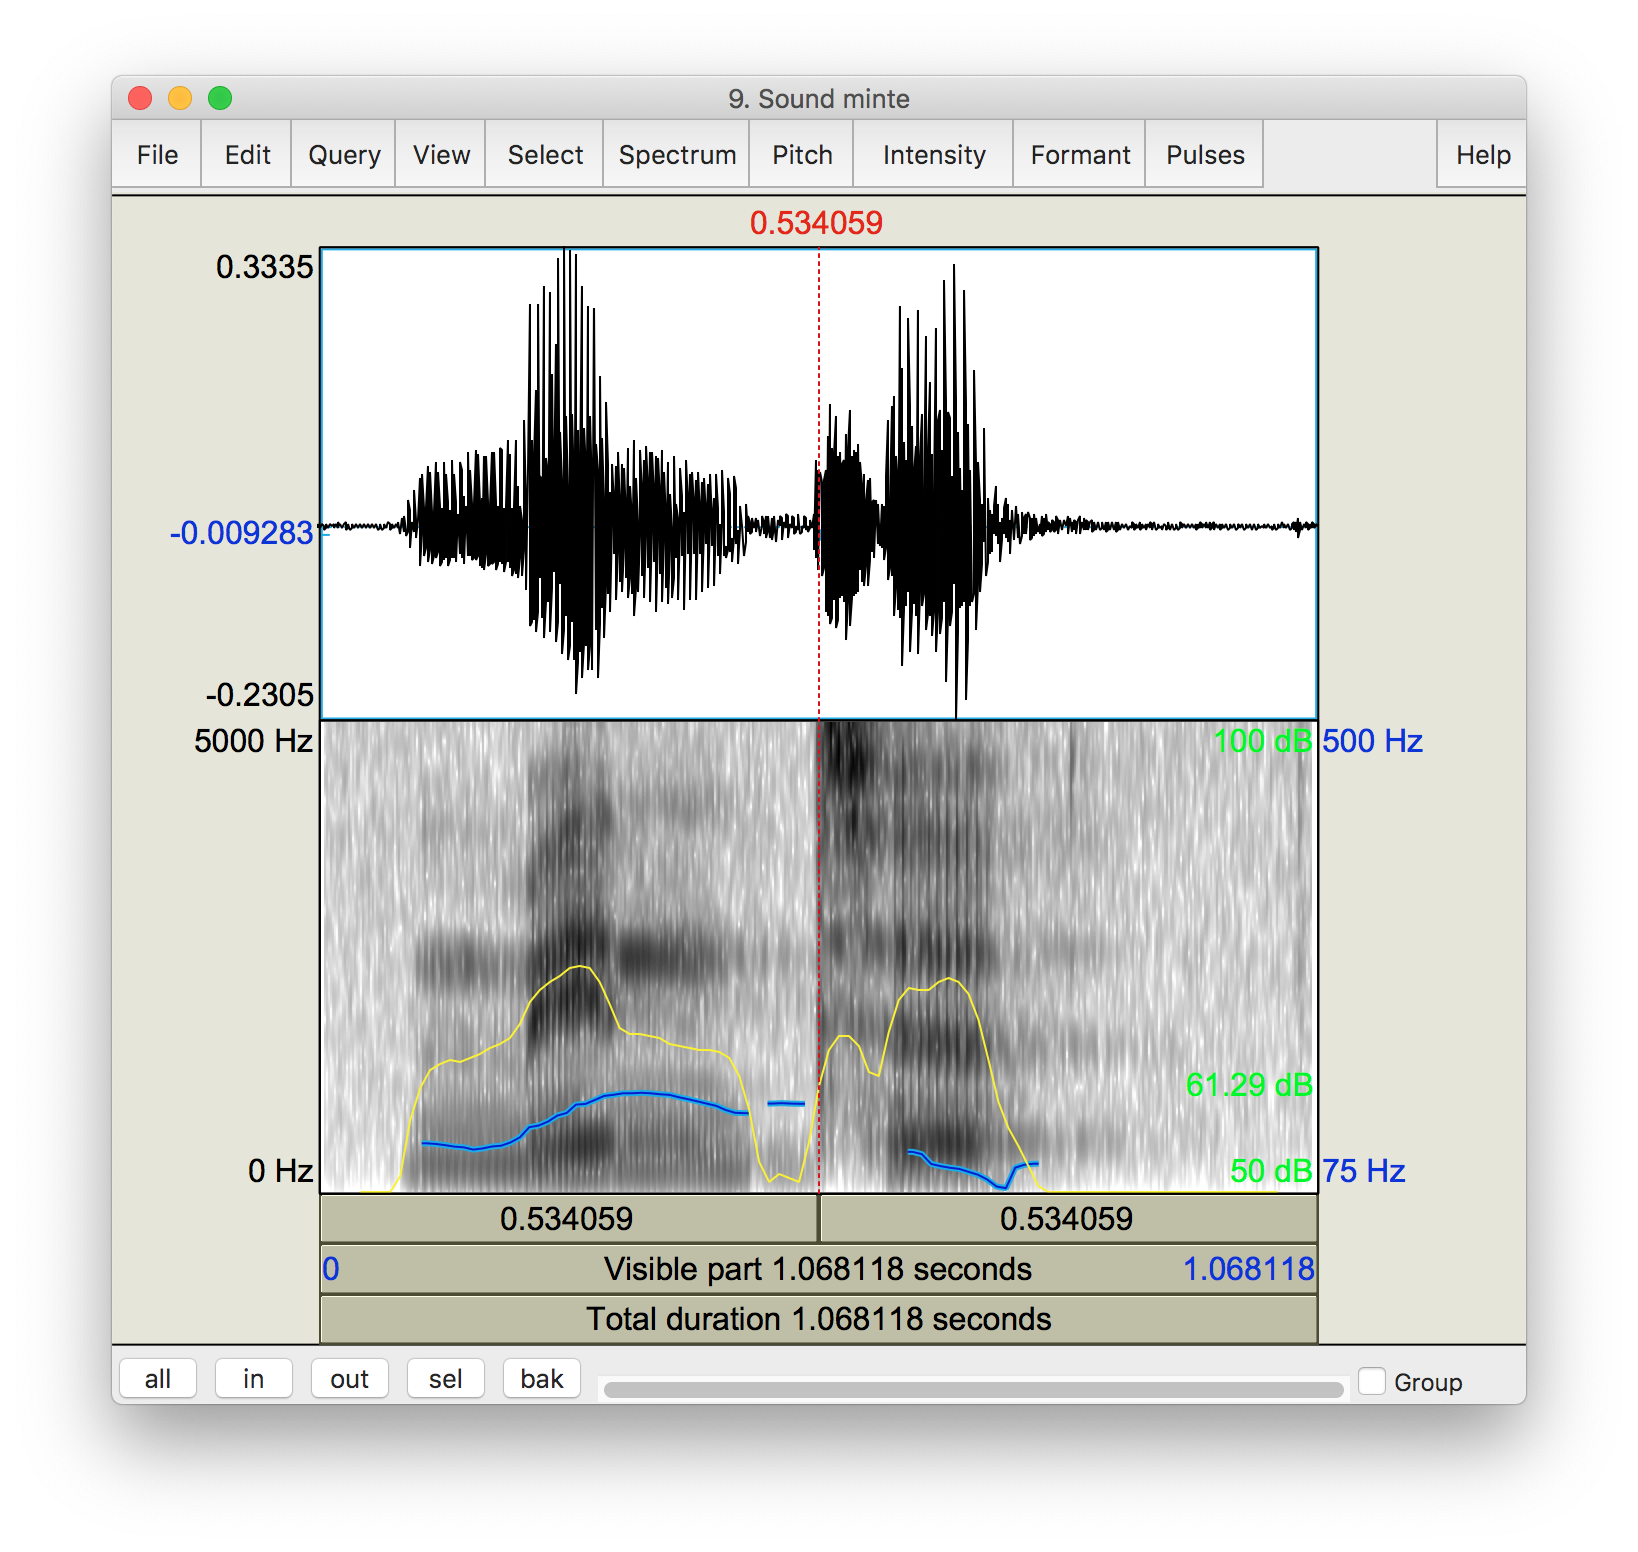
\includegraphics[height=0.8\textheight]{\GRAPHPATH/minte}
\end{frame}

\begin{frame}
  {Drucksilben und Schallsilben (Sievers, siehe \citealt{Maas2002})}
  \Large
  \textit{Miete}\\
  \Zeile
  \centering
  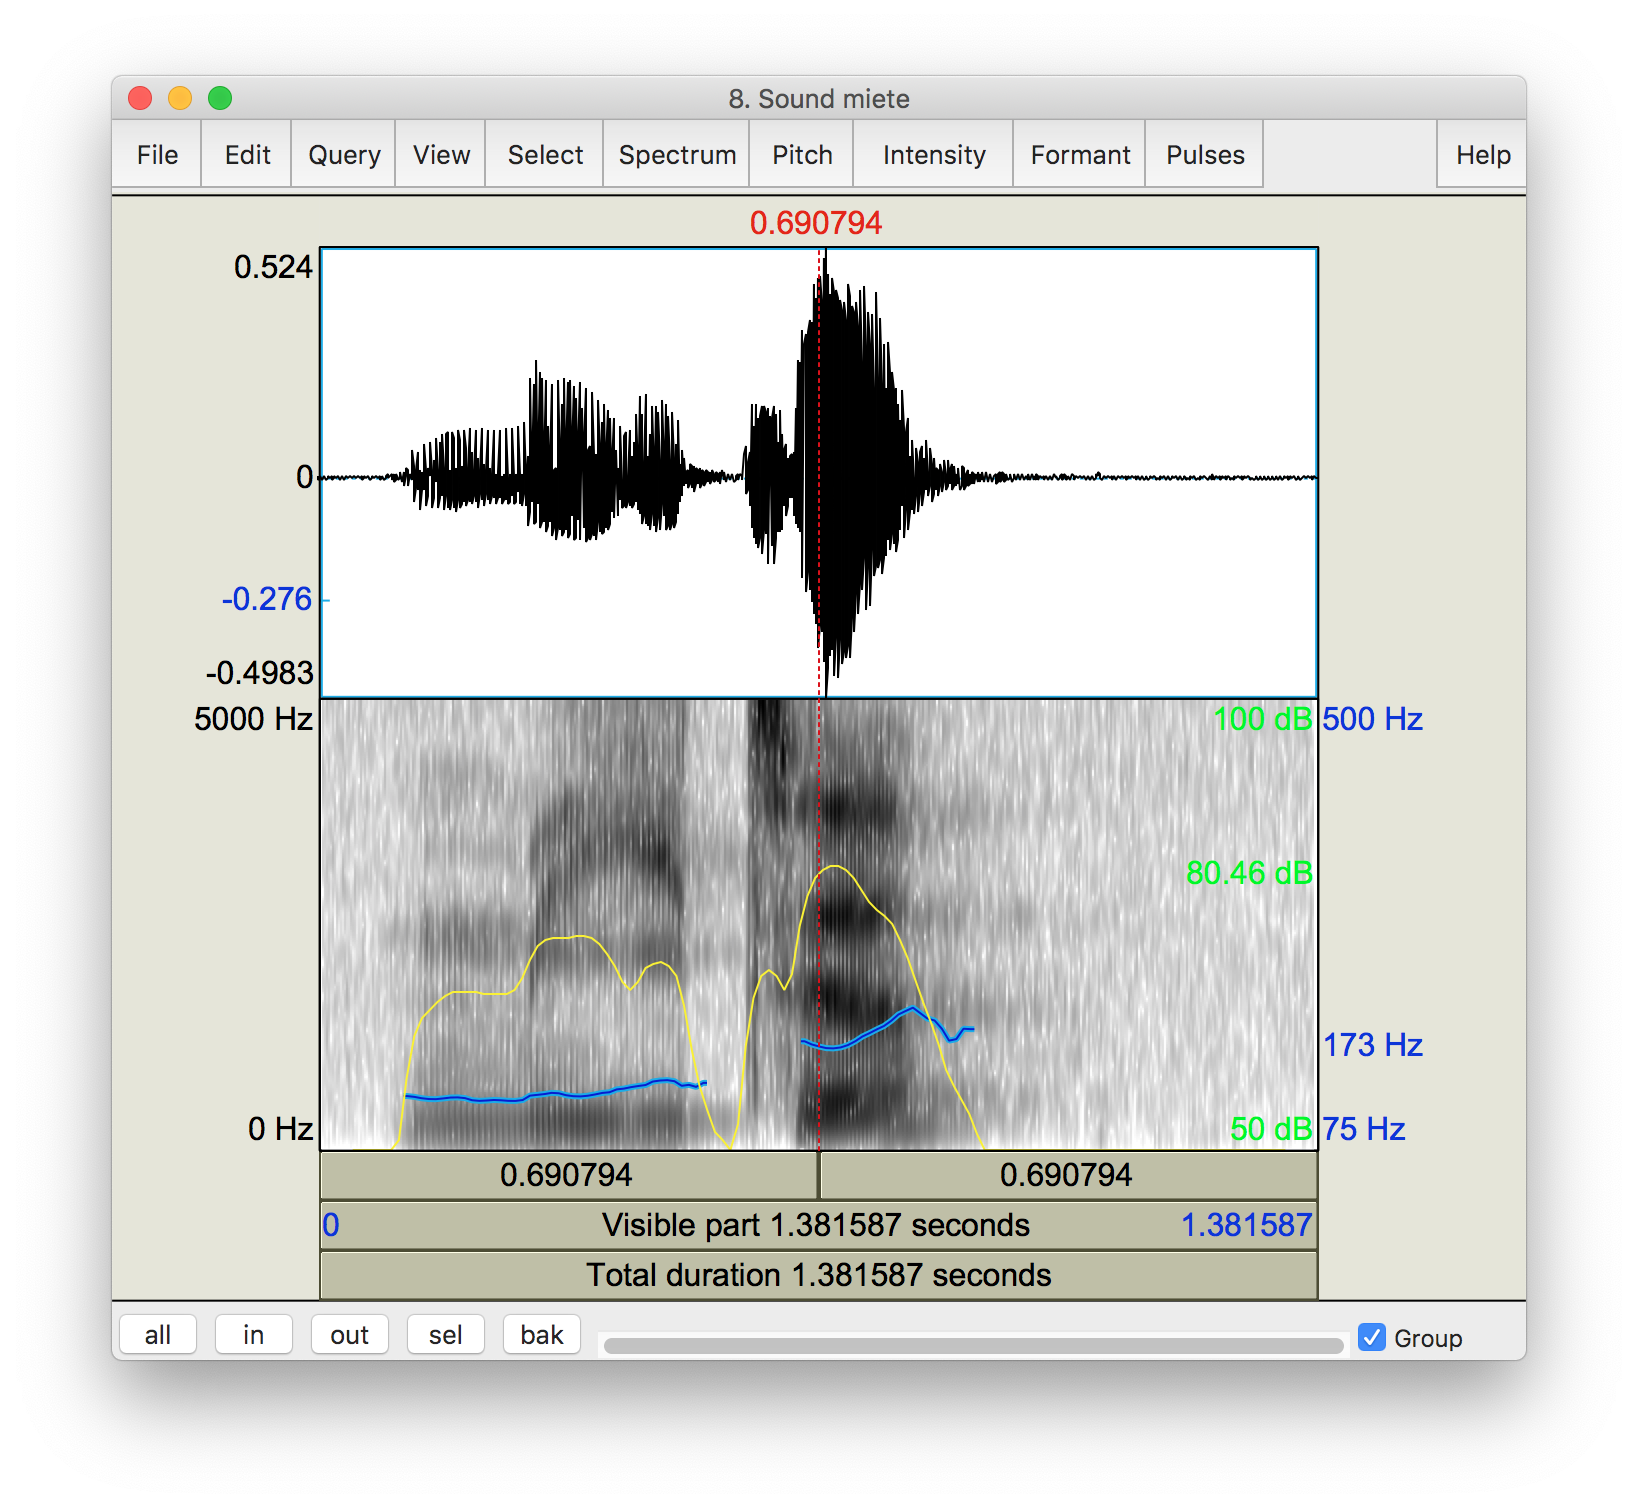
\includegraphics[height=0.8\textheight]{\GRAPHPATH/miete}
\end{frame}

\begin{frame}
  {Drucksilben und Schallsilben (Sievers, siehe \citealt{Maas2002})}
  \Large
  \textit{Mitte}\\
  \Zeile
  \centering
  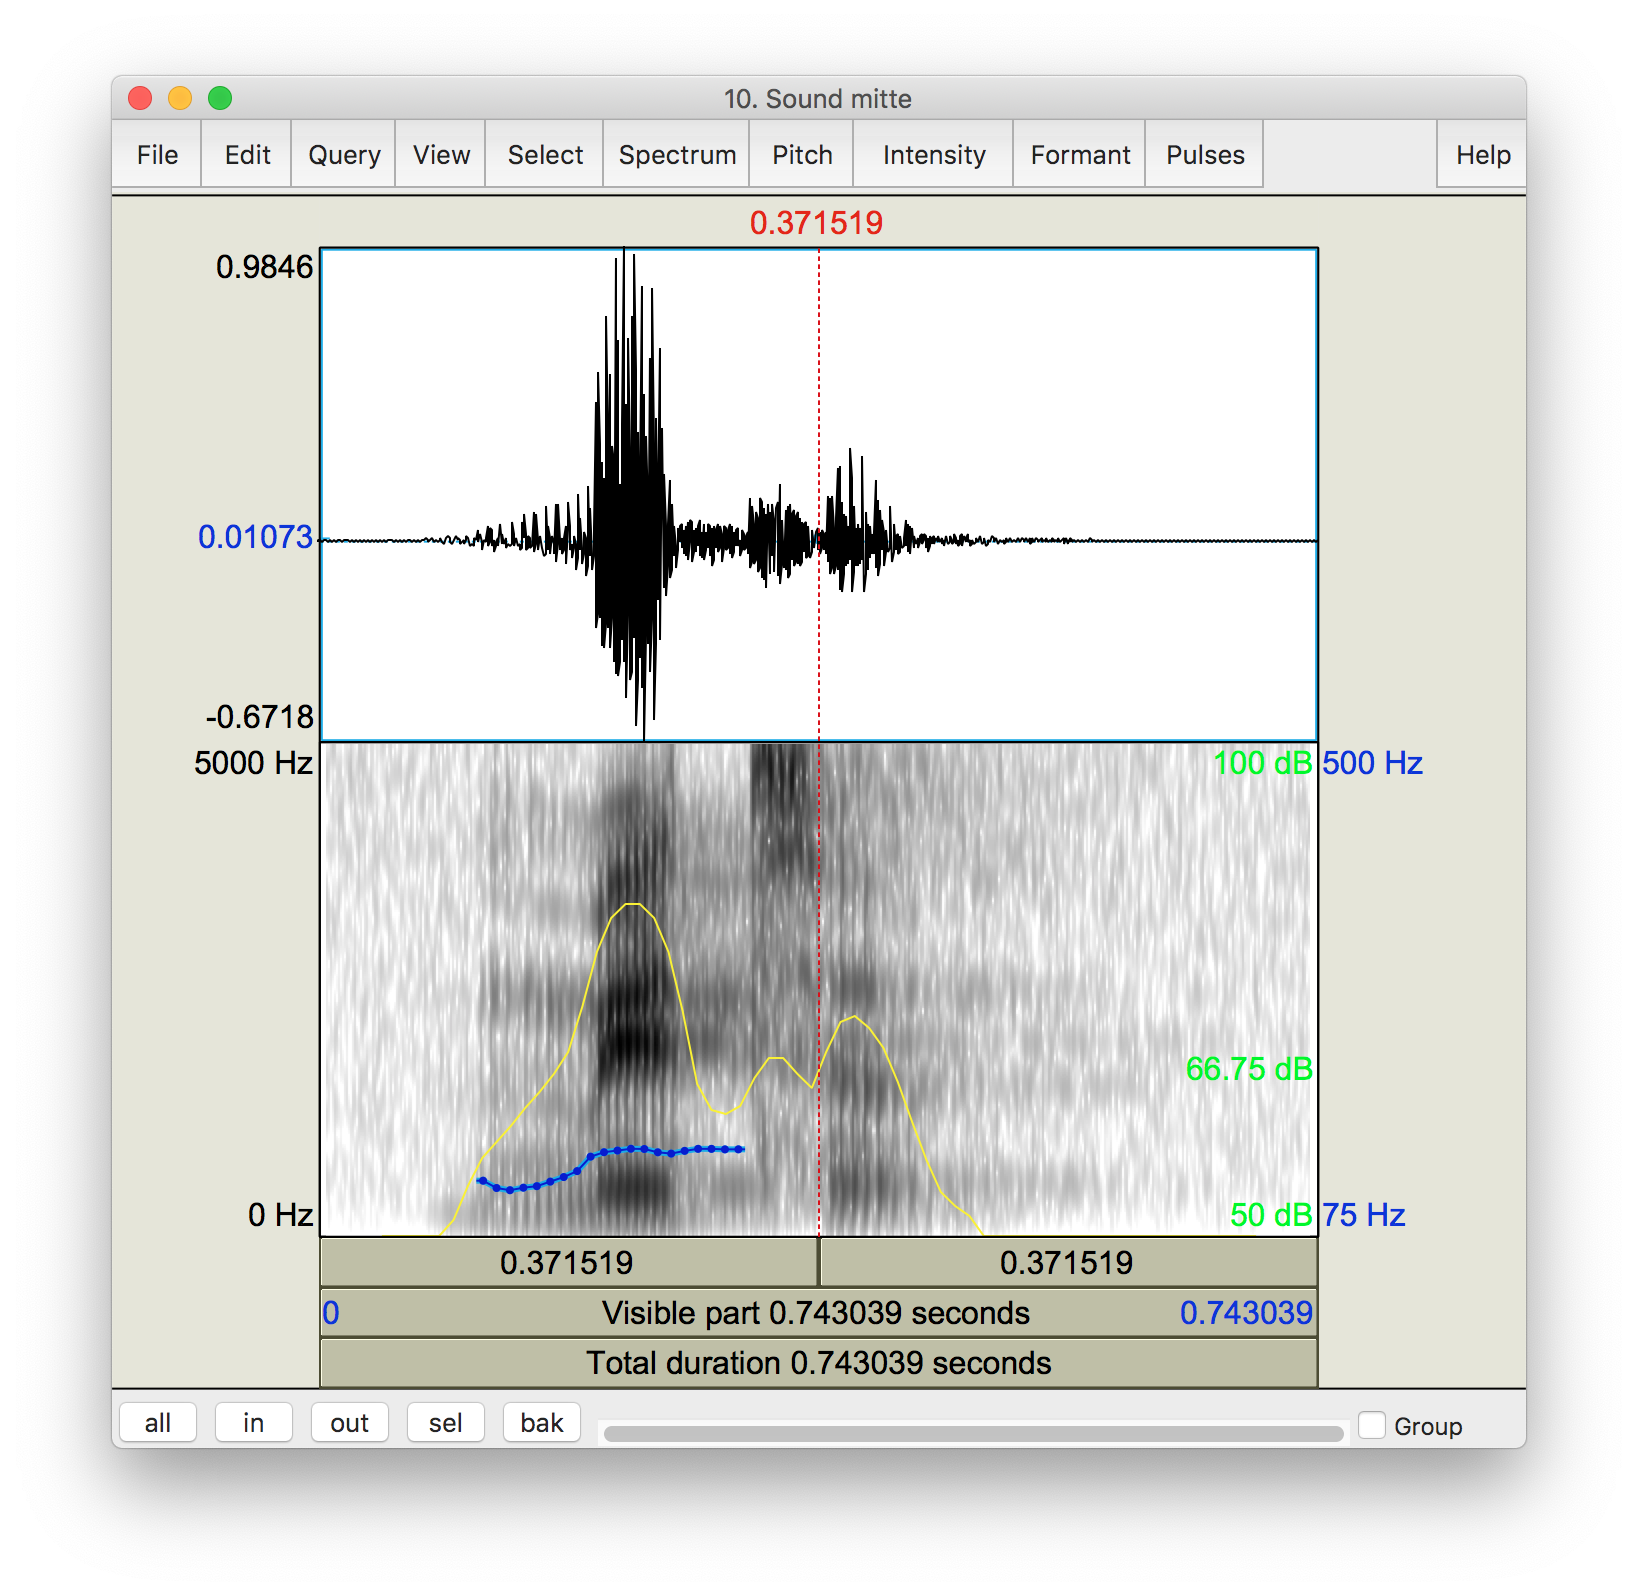
\includegraphics[height=0.8\textheight]{\GRAPHPATH/mitte}
\end{frame}

\begin{frame}
  {Nachtrag zu EGBD3}
  \pause
  In EGBD3 steht, einmorige Silben gäbe es nur mit Schwa\ldots
  \pause
  \Zeile
  \begin{itemize}[<+->]
    \item \textit{bläulichere} /blɔ͡ʏlɪçəʁə/ $\Rightarrow$ [ˈblɔ͡ʏ.l\rot{ɪ}.çə.ʁə]
    \item \textit{Neunziger} /nɔ͡ʏnt͡sɪgəʁ/ $\Rightarrow$ [ˈnɔ͡ʏn.t͡s\rot{ɪ}.gɐ]
    \item \textit{unterschiedliche} /ʊntəʁʃidlɪçə/ $\Rightarrow$ [ˈʔʊn.tɐ.ʃiːd.l\rot{ɪ}.çə]
  \end{itemize}
  \pause
  \Halbzeile
  \begin{alertblock}{Korrektur: einmorige Silben mit Nicht-Schwa}
    In abgeleiteten mehrsilbigen Wörtern können \rot{nur in unbetonten Silben}\\
    überleichte Silben mit anderen Vokalen als Schwa auftreten. Dabei wird \\
    \rot{kein Silbengelenk} gebildet. Es handelt sich im Wesentlichen um [ɪ] in\\
    abgeleiteten Adjektiven.
  \end{alertblock}
%   \pause
%   \Zeile
%   Achtung: Da \textit{-in} einen Nebenakzent trägt, liegt in \textit{Schülerinnen} /ʃyləʁɪnən/ $\Rightarrow$ [ˈʃyː.lə.ˌʁɪṇən] und ähnlichen Wörtern ein Silbengelenk vor!
\end{frame}


\begin{frame}
  {Maximierung des Anfangsrands}
  \pause
  Es bleiben immer noch Zweifelsfälle bei der wortinternen Silbifizierung\dots\\
  \pause
  \Zeile
  \begin{exe}
    \ex\textit{freches} \alert{[fʁɛç̣əs]}, \rot{*[fʁɛç.əs]}
    \pause
    \ex\textit{komplett} \alert{[kɔm.plɛt]}, \rot{*[kɔmp.lɛt]}
    \pause
    \ex\textit{Betreff} \alert{[bə.tʁɛf]}, \rot{*[bət.ʁɛf]}
  \end{exe}
  \Zeile
  \pause
  \Large
  Strukturbedingung: So viele Konsonanten wie möglich\\
  in den \alert{Anfangsrand} statt in den Endrand packen!\\
\end{frame}


\begin{frame}
  {Die Klatschmethode und die Hinhörschreibung}
  \pause
  "`Hinhörschreibungen"'?\\
  \begin{itemize}[<+->]
    \item E\rot{h}e, we\rot{h}e
    \item Ra\rot{d}, Wan\rot{d}, Bun\rot{d}
    \item bri\rot{ng}, Go\rot{ng}
    \item Köni\rot{g}, weni\rot{g}, wichti\rot{g}
    \item \rot{S}tein, \rot{S}palte
  \end{itemize}
  \pause
  "`Klatschmethode"'?\\
  \begin{itemize}[<+->]
    \item Krie\rot{ch}er, rö\rot{tl}ich, Nö\rot{rgl}er, a\rot{bsp}a\rot{lt}en, Ä\rot{rzt}e, plö\rot{tzl}ich
    \item rate, ratte
    \item Matsche
    \item Küche
    \item bringe
  \end{itemize}
\end{frame}


\begin{frame}
  {Und wie geht es richtig?}
  \pause
  \Large
  \Zeile\Zeile
  \begin{center}
    Denken Sie da mal drüber nach!
  \end{center}
%   \Halbzeile
%   Ganz allgemein wichtig für Grammatikvermittlung:\\
%  \Halbzeile 
%  \pause
%  \begin{itemize}[<+->]
%     \item Was ist die \alert{Fähigkeit}, die vermittelt werden soll?
%     \item Welches \alert{Wissen} ist nötig, um diese zu erwerben?
%     \item Welchen \alert{Übungs-Input} müssen Sie den Lernenden geben?
%   \end{itemize}
%  \Halbzeile
%  \pause
%   Mögliches Vorgehen:
%   \pause
%   \begin{itemize}[<+->]
%     \item \alert{Bewusstsein für Länge}
%     \item Bewusstsein für \alert{Länge je nach Position}
%     \item kurz vor Vokal im Wort $\Rightarrow$ Silbengelenk, Gelenkschreibung
%     \item \rot{Formenreihen als Ausgangsbasis}: \alert{nur Kernwortschatz}
%     \item Anfang mit dem \alert{Einsilbler} (ohne Dehnungsschreibung?)
%     \item weiter mit dem \alert{trochäischen Zweisilbler ohne Silbengelenk}
%     \item schließlich \alert{Zweisilbler mit Silbengelenk}
%   \end{itemize}
\end{frame}

\section{Vorschau}

\begin{frame}
  {Nächste Woche: Wortklassen und Wortarten}
  \pause
  \begin{itemize}[<+->]
    \item Was sind Wörter?
    \item Sind Wortklassen durch \alert{Bedeutungen} definiert?
    \item \alert{morphologische} Definitionen von Wortklassen
    \item \alert{syntaktische} Definitionen von Wortklassen
    \item \alert{Wie viele Wortklassen gibt es?}
  \end{itemize}
  \pause
  \Zeile
  \centering
  \Large
  \alert{Bitte lesen: Kapitel 6 komplett,\\
  mindestens aber 6.2 (S.~174--191)}
  \pause
  \pause
  \pause
  \pause
  \pause
\end{frame}


  
\section{Rückblick}

\begin{frame}
  {Silbenphonologie}
  \pause
  \begin{itemize}[<+->]
    \item Silben sind nicht lexikalisch\slash zugrundeliegend.
    \item Sonorität: Öffnen und Schließen des Vokaltrakts
    \item Sonoritätskontur: Anstieg zum Vokal, dann Abfall
    \item Anfangsrand, Kern, Endrand; Reim
    \item \alert{extrasilbische} Sonoritätsverletzungen: /ʃ/, /s/, /t/
    \item prototypischer komplexe Anfangsrand: \alert{Obstruent + Liquid}
    \item prototypischer komplexe Endrand: \alert{Liquid + Obstruent}
    \item Wichtig: \alert{Das gilt für betonte Silben im Kernwortschatz.}
    \item Silbengewicht in \alert{Moren} (Vokal: eine\slash zwei, Kons.: je eine)
    \item Überschwere: verhindert durch Extrasilbizität
    \item Silbengelenk: geteilter Konsonant statt überleichter Silbe im Trochäus
    \item Anfangsrandmaximierung bei Zweifelsfällen der Silbifizierung
  \end{itemize}
\end{frame}

\begin{frame}
  {Warum Reim?}
  \pause
  \begin{itemize}[<+->]
    \item Reim = Kern und Endrand
    \item \alert{Für das Silbengewicht zählt nur der Reim!}
    \item Prinzip: eigene Regularität → eigene Struktur
      \Zeile
    \item außerdem: literarischer \alert{Endreim}: \alert{Anfangsrand egal}
    \item und: literarischer \alert{Anfangsreim} (Stabreim): \alert{Silbenreim egal} 
  \end{itemize}
\end{frame}

\begin{frame}
  {Alfred Lichtenstein: Die Dämmerung}
  \pause
  \small
  Ein dicker Junge spielt mit einem \textbf{\rot<3>{T}\alert<3>{eich}}.\\
  Der Wind hat sich in einem Baum ge\textbf{\rot<4>{f}\alert<4>{an}}/gen.\\
  Der Himmel sieht verbummelt aus und \textbf{\rot<3>{bl}\alert<3>{eich}},\\
  Als wäre ihm die Schminke ausge\textbf{\rot<4>{g}\alert<4>{an}}/gen.\\
  \Zeile
  Auf lange Krücken schief herabge\textbf{\rot<5>{b}\alert<5>{ückt}}\\
  Und schwatzend kriechen auf dem Feld zwei \textbf{\rot<6>{L}\alert<6>{ah}}|me.\\
  Ein blonder Dichter wird vielleicht ver\textbf{\rot<5>{r}\alert<5>{ückt}}.\\
  Ein Pferdchen stolpert über eine \textbf{\rot<6>{D}\alert<6>{a}}|me.\\
  \Zeile
  An einem Fenster klebt ein fetter \textbf{\rot<7>{M}\alert<7>{ann}}.\\
  Ein Jüngling will ein weiches Weib be\textbf{\rot<8>{s}\alert<8>{u}}|chen.\\
  Ein grauer Clown zieht sich die Stiefel \textbf{\alert<7>{an}}.\\
  Ein Kinderwagen schreit und Hunde \textbf{\rot<8>{fl}\alert<8>{u}}|chen.\\
  \Zeile
  \footnotesize
  Aus: Pinthus, Kurt (Hrsg.). 1920. \textit{Menschheitsdämmerung}. Berlin: Rowohlt. S.~11.\\
  Mit | sind normale Silbengrenzen und mit / Silbengelenke markiert.
\end{frame}


\section{Überblick}

\begin{frame}
  {Überblick}
  \pause
  \begin{itemize}[<+->]
    \item Was sind Wörter?
    \item Lexikalisches vs.\ syntaktisches Wort
      \Zeile
    \item Wozu Wortklassen?
    \item \rot{Bedeutungsklassen} und Wortklassen
    \item \alert{Morphologie} von Wortklassen
    \item \alert{Syntax} von Wortklassen
      \Zeile
    \item wichtige Wortklassen
      \begin{itemize}[<+->]
        \item Nomen
        \item Verb
        \item Präposition
        \item Komplementierer
        \item Adverb
        \item Partikel
      \end{itemize}
  \end{itemize}
\end{frame}

\begin{frame}
  {Wortklassen und Bildungssprache\slash Lehramt}
  \pause
  \begin{itemize}[<+->]
    \item direkter Einfluss von Wortklassenwissen auf\\
      bildungssprachliche Fähigkeiten: \rot{keiner}
      \Zeile
    \item Sprachbetrachtung (Woche 1):
      \begin{itemize}[<+->]
        \item \rot{Form} → \alert{Funktion}
        \item \rot{systematisch}, also basierend auf \alert{Generalisierungen}
        \item essentiell für formale Generalisierungen: \alert{Wortklassen}
      \end{itemize}
      \Zeile
    \item Normfragen und Wortklassenbezug
      \begin{itemize}
        \item \alert{Substantivgroßschreibung}
        \item Nebensätze: Komplementierer, Pronomina, Kommas
        \item Flexion (Problemfälle: Konjunktiv, Adjektive usw.)
        \item \dots alles nicht ohne Wortklassen beschreibbar
      \end{itemize}
  \end{itemize}
\end{frame}

\section{Wörter}

\begin{frame}
  {Ebenen und Einheiten}
  \pause
  \begin{itemize}[<+->]
    \item Wortakzent: \textit{\alert{\textbf{Sie}}ges\alert{säu}le}\\
      $\rightarrow$ phonologisches\slash prosodisches Wort
      \Zeile
    \item Eigenschaften von Wörtern jenseits der Phonologie?
  \end{itemize}
  \Zeile
  \pause
  \begin{exe}
    \ex
    \begin{xlist}
      \ex[]{Staat-es}
      \pause
      \ex[*]{Tür-es}
    \end{xlist}
    \pause
    \Zeile
    \ex
    \begin{xlist}
      \ex[]{Der Satz ist eine grammatische Einheit.}
      \pause
      \ex[*]{Die Satz ist eine grammatische Einheit.}
    \end{xlist}
  \end{exe}
\end{frame}

\begin{frame}
  {Wört haben eine Bedeutung?}
  \pause
  \begin{exe}
    \ex \alert{Es} \alert{wird} schon wieder früh dunkel.
    \pause
    \ex Kristine denkt, \alert{dass} \alert{es} bald regnen \alert{wird}.
    \pause
    \ex Adrianna \alert{hat} gestern \alert{den} Keller inspiziert.
    \pause
    \ex Camilla \alert{und} Emma sehen \alert{sich} \alert{die} Fotos \alert{an}.
  \end{exe}
  \Zeile
  \pause
  \large
  \alert{Bedeutungstragende Wörter und Funktionswörter}
\end{frame}

\begin{frame}
  {Morphologie und Syntax}
  \pause
  \begin{itemize}[<+->]
    \item Kombinatorik für \alert{Wortbestandteile}: Morphologie
      \begin{itemize}[<+->]
        \item Wortbestandteile \zB mit \alert{Umlaut}: \textit{rot} -- \textit{röter}
        \item oder \alert{Ablaut}: \textit{heben} -- \textit{hob}
      \end{itemize}
    \item Kombinatorik für \alert{Wörter}: Syntax
      \Zeile
    \item \alert{Zirkuläre oder leere Definitionen?}
    \item \rot{Nein!} Prinzip: eigene Regularität → eigene Struktur
      \Zeile
    \item Wortbestandteile \alert{nicht trennbar}:
      \begin{itemize}
        \item \textit{heb-t}\\
          *\textit{heb mit Mühe t}
        \item \textit{Ge-hob-en-heit} \\
          *\textit{Gehoben anspruchsvolle heit}
        \item \textit{Sie geht schnell heim.}\\
          \textit{Schnell geht sie heim.}
      \end{itemize}
  \end{itemize}
\end{frame}

\begin{frame}
  {Wort und Wortform I}
  \pause
  \begin{exe}
    \ex
    \begin{xlist}
      \ex (der) Tisch
      \pause
      \ex (den) Tisch
      \pause
      \ex (dem) Tisch\alert{e}
      \pause
      \ex (des) Tisch\alert{es}
      \pause
      \ex (die) Tisch\alert{e}
      \pause
      \ex (den) Tisch\alert{en}
    \end{xlist}
  \end{exe}
  \pause
  \begin{exe}
    \ex
    \begin{xlist}
      \ex Der \_\_\_\ ist voll hässlich.
      \pause
      \ex Ich kaufe den \_\_\_ nicht.
      \pause
      \ex Wir speisten am \_\_\_\ des Bundespräsidenten.
      \pause
      \ex Der Preis des \_\_\_\ ist eine Unverschämtheit.
      \pause
      \ex Die \_\_\_\ kosten nur noch die Hälfte.
      \pause
      \ex Mit den \_\_\_\ können wir nichts mehr anfangen.
    \end{xlist}
  \end{exe}
\end{frame}

\begin{frame}
  {Wort und Wortform II}
  \pause
  \begin{block}{Wortform}
    Eine Wortform ist eine in syntaktischen Strukturen auftretende und in diesen Strukturen nicht weiter zu unterteilende Einheit.
    Die Werte der Merkmale von Wortformen sind gemäß ihrem Paradigma vollständig spezifiziert.
  \end{block}
  \Zeile
  \pause
  \begin{block}{Lexikalisches Wort}
    Das (\alert{lexikalische}) \alert{Wort} ist eine Repräsentation von paradigmatisch zusammengehörenden Wortformen.
    Für das lexikalische Wort sind die Werte nur für diejenigen Merkmale spezifiziert, die in allen Wortformen des Paradigmas dieselben Werte haben.
    Die restlichen Werte werden gemäß der Position im Paradigma bei den konkret vorkommenden Wortformen des Wortes gesetzt.
  \end{block}
\end{frame}

\section{Methode}

\begin{frame}
  {Klassische Grundschul-Wortarten}
  \pause
  \scalebox{0.85}{%
  \begin{minipage}{\textwidth}
    \begin{itemize}[<+->]
      \item Dingwort
      \item Tuwort, Tätigkeitswort
      \item Wiewort, Eigenschaftswort
      \item Umstandswort
      \item Noch besser die Vermittlungsversuche:
        \begin{itemize}[<+->]
          \item Dingwörter kann man anfassen. \onslide<8->{\rot{D'oh!}}
            \pause
          \item Wie ist die Kanzlerin? -- Katatonisch.
          \item Was macht Johanna? -- Laufen.
          \item Wie, wo oder warum schläft Johanna? -- Ruhig.
        \end{itemize}
      \item Wieso auch nicht?
        \begin{itemize}[<+->]
          \item Anfassen? Wolken, Ideen, Steckdosen, Rasierklingen, \dots
          \item *Die Kanzlerin ist ehemalig.
          \item Was macht Johanna? -- Hausaufgaben.
          \item Was tut Johanna? -- *Verlaufen. \slash *Unterliegen.
          \item *Was macht\slash tut das Yoghurt? -- Verschimmeln.
          \item Wie schläft Johanna? -- *Erstaunlicherweise.
        \end{itemize}
    \end{itemize}
  \end{minipage}
  }
\end{frame}

\begin{frame}
  {Ein paar neue Wortarten nach Bedeutungen I}
  \pause
  \begin{itemize}[<+->]
    \item "`Wie, wo, warum?"' \onslide<3->{--- Warum eigentlich nicht drei Wortarten?}
      \Halbzeile
      \pause
    \item \alert{Bewegungsverben}: \textit{laufen}, \textit{springen}, \textit{fahren}, \dots
    \item \alert{Zustandsverben}: \textit{duften}, \textit{wohnen}, \textit{liegen}, \dots
      \Halbzeile
    \item \alert{Konkreta}: \textit{Haus}, \textit{Buch}, \textit{Blume}, \textit{Stier}, \dots
    \item \alert{Abstrakta}: \textit{Konzept}, \textit{Glaube}, \textit{Wunder}, \textit{Kausalität}, \dots
    \item \alert{Zählsubstantive}: \textit{Kumquat}, \textit{Student*in}, \textit{Mikrobe}, \textit{Kneipe}, \dots
    \item \alert{Stoffsubstantive}: \textit{Wasser}, \textit{Wein}, \textit{Zement}, \textit{Mehl}, \dots
  \end{itemize}
\end{frame}

\begin{frame}
  {Ein paar neue Wortarten nach Bedeutungen II}
  \pause
  Aber Moment mal\dots\\
  \pause
  \Zeile
  \begin{exe}
    \ex
    \begin{xlist}
      \ex \alert{Wein} kann lecker sein.
      \ex \alert{Kumquats können}\slash \alert{Eine Kumquat kann} lecker sein.
    \end{xlist}
%     \pause
%     \ex
%     \begin{xlist}
%       \ex Ein Glas \alert{guter Wein}\slash\alert{guten Weins} kostet 10€.
%       \ex Ein Glas \alert{?gute Kumquats}\slash\alert{guter Kumquats} kostet 4€.
%     \end{xlist}
%     \pause
%     \ex
%     \begin{xlist}
%       \ex Johanna hätte gerne \alert{eine Kumquat}.
%       \ex Johanna hätter gerne \alert{einen Wein}.
%     \end{xlist}
  \end{exe}
  \pause
  \Zeile
  Es gibt hier durchaus auch \alert{formale} Unterschiede.
\end{frame}

\begin{frame}
  {Morphologische Klassifikation}
  \pause
  \begin{exe}
    \ex
    \begin{xlist}
      \ex{Ich pfeif\alert{e}.\\
      Du pfeif\alert{st}.\\
      Die Schiedsrichterin pfeif\alert{t}.}
        \pause
        \ex{Ich schlaf\alert{e}.\\
        {Du schl\rot{ä}f\alert{st}.}\\
        Die Schiedsrichterin schl\rot{ä}f\alert{t}.}
    \end{xlist}
        \pause
    \ex
    \begin{xlist}
      \ex{der Berg\\
        des Berg\alert{es}\\
        die Berg\alert{e}}
        \pause
      \ex{der Mensch\\
        des Mensch\alert{en}\\
        die Mensch\alert{en}}
        \pause
      \ex{der Staat\\
        des Staat\alert{es}\\
        die Staat\alert{en}}
    \end{xlist}
  \end{exe}
\end{frame}

\begin{frame}
  {Achtung!}
  \pause
  \alert{Änderung der Paradigmenzugehörigkeit} eines Wortes:
  \pause
  \Zeile
  \begin{exe}
    \ex\label{ex:paradigmatischeklassifikation017}\begin{xlist}
      \ex{Wir sind des \alert{Wanderns} müde.}
      \pause
      \ex{Wir \alert{wandern}.}
    \end{xlist}
  \end{exe}
  \pause
  \Zeile
  $\Rightarrow$ \rot{Zwei verschiedene} lexikalische Wörter.
\end{frame}


\begin{frame}
  {Syntaktische Klassifikation}
  \pause
  \begin{exe}
    \ex
    \begin{xlist}
      \ex[]{Alexandra spielt schnell \alert{und} präzise.}
      \pause
      \ex[*]{Alexandra spielt schnell \alert{obwohl} präzise.}
      \pause
      \ex[]{Alexandra \alert{und} Dzsenifer spielen eine gute Saison.}
      \pause
      \ex[*]{Alexandra \alert{obwohl} Dzsenifer spielen eine gute Saison.}
    \end{xlist}
    \pause
    \Zeile
    \ex
    \begin{xlist}
      \ex[]{Alexandra spielt herausragend,\\
        \alert{obwohl} der Leistungsdruck hoch ist.}
      \pause
      \ex[*]{Alexandra spielt herausragend, \alert{und} der Leistungsdruck hoch ist.}
    \end{xlist}
  \end{exe}
    \pause
    \Zeile
    Alles nur wegen der Bedeutung?
    \pause
  \begin{exe}
    \ex Der Marmorkuchen spielt schnell \alert{und} präzise.
  \end{exe}
\end{frame}

\begin{frame}[fragile]
  {Filter}
  \begin{itemize}
    \item<2-> Kapitel 2: \alert{Kategorien} definiert über Merkmale und Werte.
      \begin{itemize}[<+->]
        \item<3-> Hat \textsc{Numerus} oder nicht?
        \item<4-> Hat \textsc{Genus} oder nicht?
        \item<5-> \dots
      \end{itemize}
  \end{itemize}
  \begin{center}
    \scalebox{0.7}{
    \begin{minipage}{\textwidth}  
    \begin{forest}
      /tikz/every node/.append style={font=\footnotesize},
      for tree={l sep=2em, s sep=2.5em},
      [\textit{Wort}, intrme, {visible on=<6->}, for children={visible on=<7->}
        [{Hat  Numerus?}, decide, for children={visible on=<8->}
          [\textit{flektierbar}, intrme, yes, {visible on=<9->}, for children={visible on=<11->}
            [{Ist finit  flektierbar?}, decide, {visible on=<11->}, for children={visible on=<12->}
              [\textbf{Verb}, finall, yes, {visible on=<13->}]
              [\textit{Nomen}, intrme, no, {visible on=<14->}]
            ]
          ]
          [\textit{nicht flektierbar}, intrme, no, {visible on=<10->}, for children={visible on=<15->}
            [{Hat Valenz-\slash  Kasusrektion?}, decide, {visible on=<15->}, for children={visible on=<16->}
              [\textbf{Präposition}, finall, yes, {visible on=<17->}]
              [\textit{andere}, intrme, no, {visible on=<18->}]
            ]
          ]
        ]
      ]
    \end{forest}
   \end{minipage}
   }
  \end{center}
\end{frame}


\section{Wortklassen}

\begin{frame}
  {Flektierbare Wörter: Numerus}
  \pause
  \begin{exe}
    \ex
    \begin{xlist}
      \ex Tüte, Tüten
      \pause
      \ex Baum, Bäume
    \end{xlist}
    \pause
    \ex
    \begin{xlist}
      \ex (ich) gehe, (wir) gehen
      \pause
      \ex (du) gehst, (ihr) geht
    \end{xlist}
    \Zeile
    \pause
    \ex
    \begin{xlist}
      \ex \alert<12->{Ein} \alert<13->{roter} \alert<8->{Apfel} \alert<9->{hängt} am Baum.
      \pause
      \ex \alert<14->{Rote} \alert<10->{Äpfel} \alert<11->{hängen} am Baum.
    \end{xlist}
  \end{exe}
  \Zeile
  \pause
  \pause
  \pause
  \pause
  \pause
  \pause
  \pause
  \pause
  Als \alert{Kongruenzmerkmal} ist Numerus in der Definition\\
  der flektierbaren Wortklassen \alert{strukturell motiviert}.
\end{frame}

\begin{frame}
  {Substantive vs.\ Nomina}
  \pause
  \begin{exe}
    \ex \alert<5->{Die stärkste} Gewichtheberin wurde Weltmeisterin.
    \pause
    \ex \alert<5->{Der stärkste} Versuch war der zweite.
    \pause
    \ex \alert<5->{Das höchste} Gewicht wurde von Tatjana gerissen.
  \end{exe}
  \Zeile
  \pause
  \pause
  \begin{itemize}[<+->]
    \item Substantive: festes Genus
    \item andere Nomina (Artikel\slash Pronomen, Adjektiv):\\
      \alert{Genuskongruenz mit dem Substantiv}
  \end{itemize}
\end{frame}

\begin{frame}
  {Adjektive}
  \pause
  \begin{exe}
    \ex
    \begin{xlist}
      \ex Kein \alert<3->{großer} Ball wurde gespielt.
      \ex Der \alert<3->{große} Ball wurde gespielt.
    \end{xlist}
    \pause
    \pause
    \ex
    \begin{xlist}
      \ex Keine \alert<5->{großen} Bälle wurden gespielt.
      \ex Die \alert<5->{großen} Bälle wurden gespielt.
      \ex Große \alert<5->{Bälle} wurden gespielt.
    \end{xlist}
  \end{exe}
  \Zeile
  \pause
  \pause
  \centering
  \resizebox{0.4\textwidth}{!}{
    \begin{tabular}{lllllll}
      \toprule
      \multicolumn{3}{l}{} & \textbf{Mask} & \textbf{Neut} & \textbf{Fem} & \textbf{Pl} \\
      \midrule
      \multirow{4}{*}{\textbf{stark}} & \textbf{Nom} & \multirow{4}{*}{heiß-} & er & es & e & e \\
      & \textbf{Akk} && en & es & e & e \\
      & \textbf{Dat} && em & em & er & en \\
      & \textbf{Gen} && en & en & er & er \\
      \midrule
      \multirow{4}{*}{\textbf{schwach}} & \textbf{Nom} & \multirow{4}{*}{(der) heiß-} & e & e & e & en \\
      & \textbf{Akk} && en & e & e & en \\
      & \textbf{Dat} && en & en & en & en \\
      & \textbf{Gen} && en & en & en & en \\
      \midrule
      \multirow{4}{*}{\textbf{gemischt}} & \textbf{Nom} & \multirow{4}{*}{(kein) heiß-} & er \Dim & es \Dim & e & en \\
      & \textbf{Akk} && en & es \Dim & e & en \\
      & \textbf{Dat} && en & en & en & en \\
      & \textbf{Gen} && en & en & en & en \\
      \bottomrule
    \end{tabular}
  }
\end{frame}

\begin{frame}
  {Präpositionen}
  \pause
  \begin{exe}
    \ex
    \begin{xlist}
      \ex{\alert<3-4>{Mit} \alert<4>{dem kaputten Rasen} ist nichts mehr anzufangen.}
      \pause
      \pause
      \pause
      \ex{\alert<6-7>{Angesichts} \alert<7>{des kaputten Rasens} wurde das Spiel abgesagt.}
    \end{xlist}
  \end{exe}
  \pause
  \pause
  \pause
  \Zeile
  \begin{block}{Rektion}
    In einer Rektionsrelation werden durch die regierende Einheit (das \alert{Regens}) Werte für bestimmte Merkmale (und ggf.\ auch die Form) beim regierten Element (dem \alert{Rectum}) verlangt.\\
  \end{block}
  \Zeile
  \pause
  \begin{block}{Präposition}
    Präpositionen kasusregieren eine obligatorische Nominalphrase.
  \end{block}
\end{frame}

\begin{frame}
  {Komplementierer}
  \pause
  \begin{exe}
    \ex
    \begin{xlist}
      \ex[]{Ich glaube, [\alert<3->{dass} dieser Nebensatz ein Verb \alert<4->{enthält}].}
      \ex[]{[\alert<6->{Während} die Spielzeit \alert<7->{läuft}], zählt jedes Tor.}
      \ex[]{Es fällt ihnen schwer [\rot<8->{zu laufen}].}
      \ex[\rot<11->{*}]{[\alert<9->{Obwohl} kein Tor \alert<10->{fiel}].}
    \end{xlist}
  \end{exe}
  \Zeile
  \pause
  \pause
  \pause
  \pause
  \pause
  \pause
  \pause
  \pause
  \pause
  \pause
  \begin{block}{Komplementierer}
    Komplementierer leiten Nebensätze ein.\\
    Die Rede von der \textit{unterordnenden Konjunktion} ist ungeschickt.
  \end{block}
\end{frame}

\begin{frame}
  {Nicht-flektierbare Wörter im Vorfeld}
  \pause
  Was steht im unabhängigen Aussagesatz am Satzanfang?\\
  \pause
  {\rot{Antworten Sie nie mehr mit "`das Subjekt"'!}}
  \pause
  \begin{exe}
    \ex\label{ex:adverbenadkopulasundpartikeln038}
    \begin{xlist}
      \ex[ ]{\alert<5->{Gestern} hat der FCR Duisburg gewonnen.}
      \pause
      \pause
      \ex[ ]{\alert<7->{Erfreulicherweise} hat der FCR Duisburg gestern gewonnen.}
      \pause
      \pause
      \ex[ ]{\alert<9->{Oben} finden wir andere Beispiele.}
      \pause
      \pause
      \ex[*]{\alert<11->{Doch} ist das aber nicht das Ende der Saison.}
      \pause
      \pause
      \ex[*]{\alert<13->{Und} ist die Saison zuende.}
      \pause
      \pause
    \end{xlist}
    \ex\label{ex:adverbenadkopulasundpartikeln044} Das ist aber \alert{doch} nicht das Ende der Saison.
  \end{exe}
  \pause
  \Viertelzeile
  \begin{block}{Adverb}
    Adverben sind die übriggebliebenen nicht-flektierbaren Wörter, die im Vorfeld stehen können.
  \end{block}
\end{frame}

\begin{frame}
  {Adkopulas}
  \pause
  Kopulas: \textit{sein}, \textit{bleiben}, \textit{werden}\\
  \pause
  Spezielle Klasse von Hilfsverben\dots
  \pause
  \Zeile
  \begin{exe}
    \ex
    \begin{xlist}
      \ex[ ]{Hamlet \alert<6->{ist} \alert<5->{meschugge}.}
      \pause
      \pause
      \pause
      \ex[ ]{\alert<8->{Quitt} \alert<9->{bin} ich mit dir noch lange nicht.}
      \pause
      \pause
      \pause
    \end{xlist}
    \Zeile
    \ex
    \begin{xlist}
      \ex[ ]{Tatjana \alert<11->{ist} \alert<12->{stark}.}
      \pause
      \pause
      \pause
      \ex[ ]{Die \alert<14->{starke} \alert<15->{Gewichtheberin} ist Weltmeisterin.}
      \pause
      \pause
      \pause
    \end{xlist}
    \Zeile
    \ex
    \begin{xlist}
      \ex[ ]{Der Staat \alert<18->{ist} \alert<17->{pleite}.}
      \pause
      \pause
      \pause
      \ex[*]{Der \alert<20->{pleite} \alert<21->{Staat} bricht zusammen.}
      \pause
      \pause
      \pause
    \end{xlist}
  \end{exe}
  \begin{block}{Adkopula}
    Adkopulas treten immer in Abhängigkeit einer Kopula auf.
  \end{block}
\end{frame}

\begin{frame}
  {Konjunktionen}
  \pause
  \begin{exe}
    \ex\label{ex:konjunktionen052}
    \begin{xlist}
      \ex{[Dzsenifer] \alert<3->{und} [eine andere Spielerin] haben Tore geschossen.}
      \pause
      \pause
      \ex{Sätze können wir [aufschreiben] \alert<5->{oder} [aussprechen].}
      \pause
      \pause
      \ex{Spielt bitte [konzentriert] \alert<7->{und} [offensiv].}
      \pause
      \pause
    \end{xlist}
  \end{exe}
  \Zeile
  \begin{block}{Konjunktion}
    Konjunktionen verbinden Satzteile der gleichen Kategorie.\\
    Die Rede von der \textit{neben-}\slash\textit{beiordnenden Konjunktion} ist ungeschickt. 
  \end{block}
\end{frame}

\begin{frame}[fragile]
  {"`Alle Wortklassen"'}
  \pause
  \begin{center}
    \scalebox{0.35}{
    \begin{minipage}{\textwidth}
    \centering
    \begin{forest}
      /tikz/every node/.append style={font=\footnotesize},
      for tree={l sep=2em, s sep=2.5em, align=center},
      [\textit{Wort}, intrme
        [{Hat\\Numerus?}, decide
          [\textit{flektierbar}, intrme, yes
            [{Ist finit\\flektierbar?}, decide
              [\textbf{Verb}, finall, yes]
              [\textit{Nomen}, intrme, no
                [{Hat festes\\Genus?}, decide
                  [\textbf{Substantiv}, finall, yes]
                  [{\textit{anderes}\\\textit{Nomen}}, intrme, no
                    [{Hat Stärke-\\flexion?}, decide
                      [\textbf{Adjektiv}, finall, yes]
                      [{\textit{Artikel\slash}\\\textit{Pronomen}}, intrme, no]
                    ]
                  ]
                ]
              ]
            ]
          ]
          [\textit{nicht flektierbar}, intrme, no
          [{Hat Valenz-\slash\\Kasusrektion?}, decide
              [\textbf{Präposition}, finall, yes]
              [\textit{andere}, intrme, no
                [{Leitet Neben-\\Sätze ein?}, decide
                  [\textbf{Komplementierer}, finall, yes]
                  [{\textit{Partikel\slash}\\\textit{Adverb}}, intrme, no
                    [{Kann das Vor-\\feld besetzen?}, decide
                      [{\textit{Adverb\slash}\\\textit{Adkopula}}, intrme, yes
                        [{Wird typisch mit\\Kopula verwendet?}, decide
                          [\textbf{Adkopula}, finall, yes]
                          [\textbf{Adverb}, finall, no]
                        ]
                      ]
                      [\textit{Partikel}, intrme, no
                        [{Kann Sätze\\ersetzen?}, decide
                          [\textbf{Satzäquivalent}, finall, yes]
                          [\textit{andere}, intrme, no
                            [{Kann Konsti-\\tuenten verbinden?}, decide
                              [\textbf{Konjunktion}, finall, yes]
                              [\textit{Rest}, intrme, no]
                            ]
                          ]
                        ]
                      ]
                    ]
                  ]
                ]
              ]
            ]
          ]
        ]
      ]
    \end{forest}
    \end{minipage}
    }
  \end{center}
\end{frame}

\begin{frame}
  {Wie viele Wortklassen gibt es?}
  \pause
  \begin{itemize}[<+->]
    \item Alle Wörter sind \alert{Wörter}.
    \item Also gibt es \rot{eine Wortklasse}.
      \Zeile
    \item Jedes Wort hat \alert{individuelle Eigenschaften}.
    \item Also gibt es \rot{so viele Wortklassen wie Wörter}.
      \Zeile
    \item Wozu brauchen wie überhaupt Wortklassen?\\
      Wortklassen\dots
      \begin{itemize}[<+->]
        \item \dots sind \alert{das Rüstzeug für Morphologie und Syntax}.
        \item \dots erlauben die Formulierung von \rot{Generalisierungen}.
        \item \dots sind so fein unterteilt, wie es unsere Beschreibung erfordert.
        \item \dots sind \rot{nicht universell}!
        \item \dots sind \alert{Artefakte unserer Theorie bzw.\ Grammatik}.
      \end{itemize}
  \end{itemize}
\end{frame}

\section{Vorschau}

\begin{frame}
  {Morphologie}
  \pause
  \textit{"`Das ist wegen der Spannendheit."'}\\
  \pause
  \textit{"`Die Vase ist vollansichtlich reliefiert."}\\
  \Zeile
  \pause
  \begin{itemize}[<+->]
    \item (Wort-)Formen, ihre Bestandteile und ihre Funktionen
    \item Umlaut und Ablaut und ihre Funktionen
    \item Unterschied von Flexion und Wortbildung
      \Zeile
    \item Funktion nominaler Flexionskategorien
    \item \rot{Wichtig!} \alert{Inklusive: Was ist Kasus?}
    \item Funktionen verbaler Flexionskategorien
    \item \rot{Wichtig!} \alert{Inklusive: Was ist Tempus?}
  \end{itemize}
  \pause
  \Zeile
  \centering
  Bitte lesen: \alert{Kapitel 7 (195--220), 9.1 (248--257), 10.1 (287--299)}

  \pause
  \pause
  \pause
  \pause
  \pause
\end{frame}


  
\section{Rückblick}

\begin{frame}
  {Wortklassen: Grundlagen}
  \pause
  \begin{itemize}[<+->]
    \item Wortklassen als \alert{Grundausstattung der Grammatik}
    \item Vehikel für klassenbezogene Generalisierungen
    \item Bedeutung? --- nicht alle Wörter
      \Zeile
    \item Wortform\slash syntaktisches Wort:
      \begin{itemize}[<+->]
        \item konkrete Form \alert{im syntaktischen Kontext}
        \item voll spezifiziert (Merkmale, Werte)
      \end{itemize}
      \Zeile
    \item Wort\slash lexikalisches Wort:
      \begin{itemize}[<+->]
        \item abstrakte Form \alert{im Lexikon}
        \item evtl.\ unterspezifiziert
      \end{itemize}
      \Zeile
    \item "`Schulwortarten"': \alert{unzureichend operationalisiert}
  \end{itemize}
\end{frame}

\section{Überblick}

\begin{frame}
  {Morphologie: Flexion und Wortbildung}
  \pause
  \begin{itemize}[<+->]
    \item \alert{Formveränderungen} und \alert{Merkmalsänderungen}
      \begin{itemize}[<+->]
        \item Veränderungen von Werten
        \item Veränderungen von Merkmalsaustattungen
      \end{itemize}
      \Halbzeile
    \item Morphe (= Wortbestandteile) und ihre Funktionen
    \item Morphe: alle Stämme und alle nicht-lexikalischen Morphe
    \item Umlaut und Ablaut (bzw.\ Vokalstufen)
      \Halbzeile
    \item statische und volatile Merkmale
    \item Wortbildung vs.\ Flexion, definiert anhand von Merkmalen
  \end{itemize}
\end{frame}

\begin{frame}
  {Morphologie und Bildungssprache\slash Normsprache}
  \pause
  \begin{itemize}[<+->]
    \item Flexion und zugehörige Funktionskategorien
      \begin{itemize}[<+->]
        \item normsprachlich überwiegend \alert{klar definiert}
        \item vorliterate perfekte Beherrschung nicht voraussetzbar (z.\,B.\ Konjunktiv)
          \Halbzeile
        \item erhebliche Abweichungen in \alert{Dialekten}, \alert{Soziolekten} und \alert{Kiezsprachen}
          \Halbzeile
        \item \textit{Et rēchnet aufe Terasse.} (Pott)
        \item Aber wie funktioniert das eigentlich genau?
          \Halbzeile
        \item \textit{Ich las schon einmal Rilke.} (rhfr. Hyperkorrektur)
        \item Im Odenwald gibt es kein Präteritum, wird in der Schule gelernt.
      \end{itemize}
     \Halbzeile 
    \item Wortbildung
      \begin{itemize}[<+->]
        \item wichtiger Kern der Bildungssprache (besonders Komposition)
          \Halbzeile
        \item \textit{Das ist wegen der Spannendheit.} (Kind, 7--8 Jahre, ca. 1992)
        \item \textit{Die Vase ist vollansichtlich reliefiert.} (Heide Rezepa-Zabel, 2018)
      \end{itemize}
  \end{itemize}
\end{frame}

\begin{frame}
  {Morphosyntax in der Schule}
  \pause
  Wozu ist so ein Unterricht gut?
  \pause
  \begin{center}
    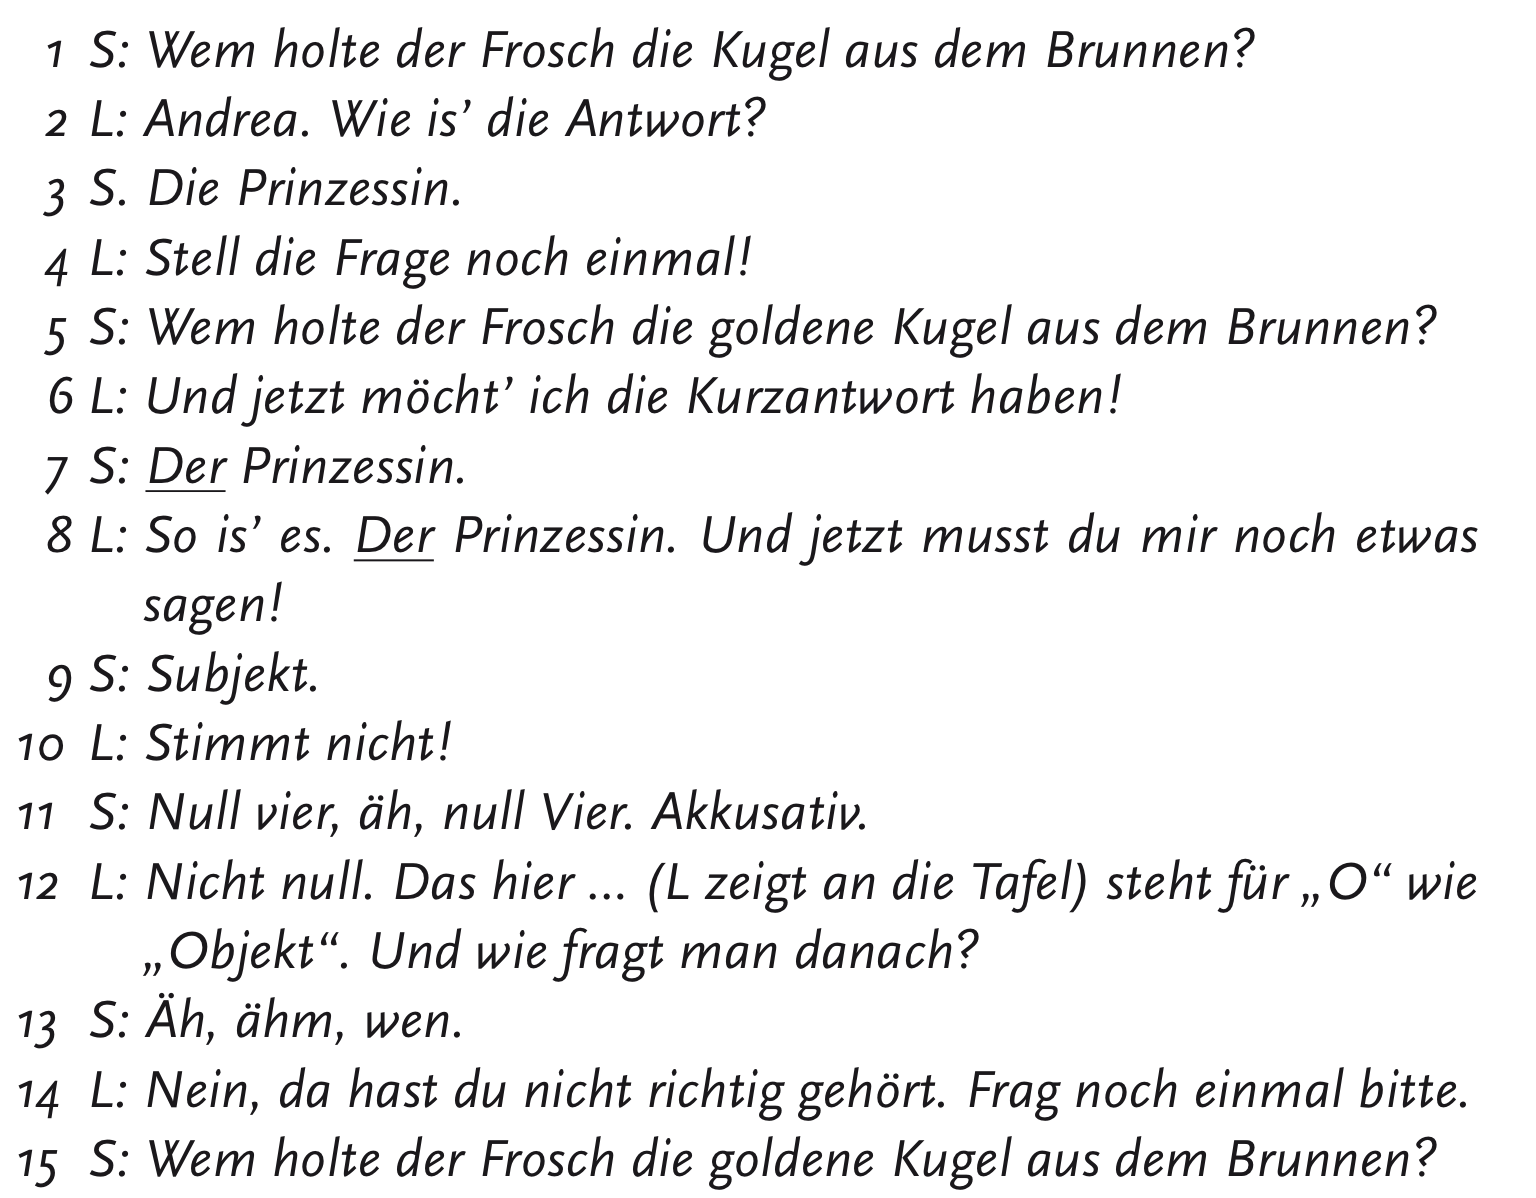
\includegraphics[width=0.6\textwidth]{graphics/kasusschule1}
  \end{center}
  \tiny \citet[36--37]{Gramzowemden2002}, zitiert nach \citet[257--258]{Bredel2013}
\end{frame}

\begin{frame}
  {Morphosyntax in der Schule}
  Wozu ist so ein Unterricht gut?
  \begin{center}
    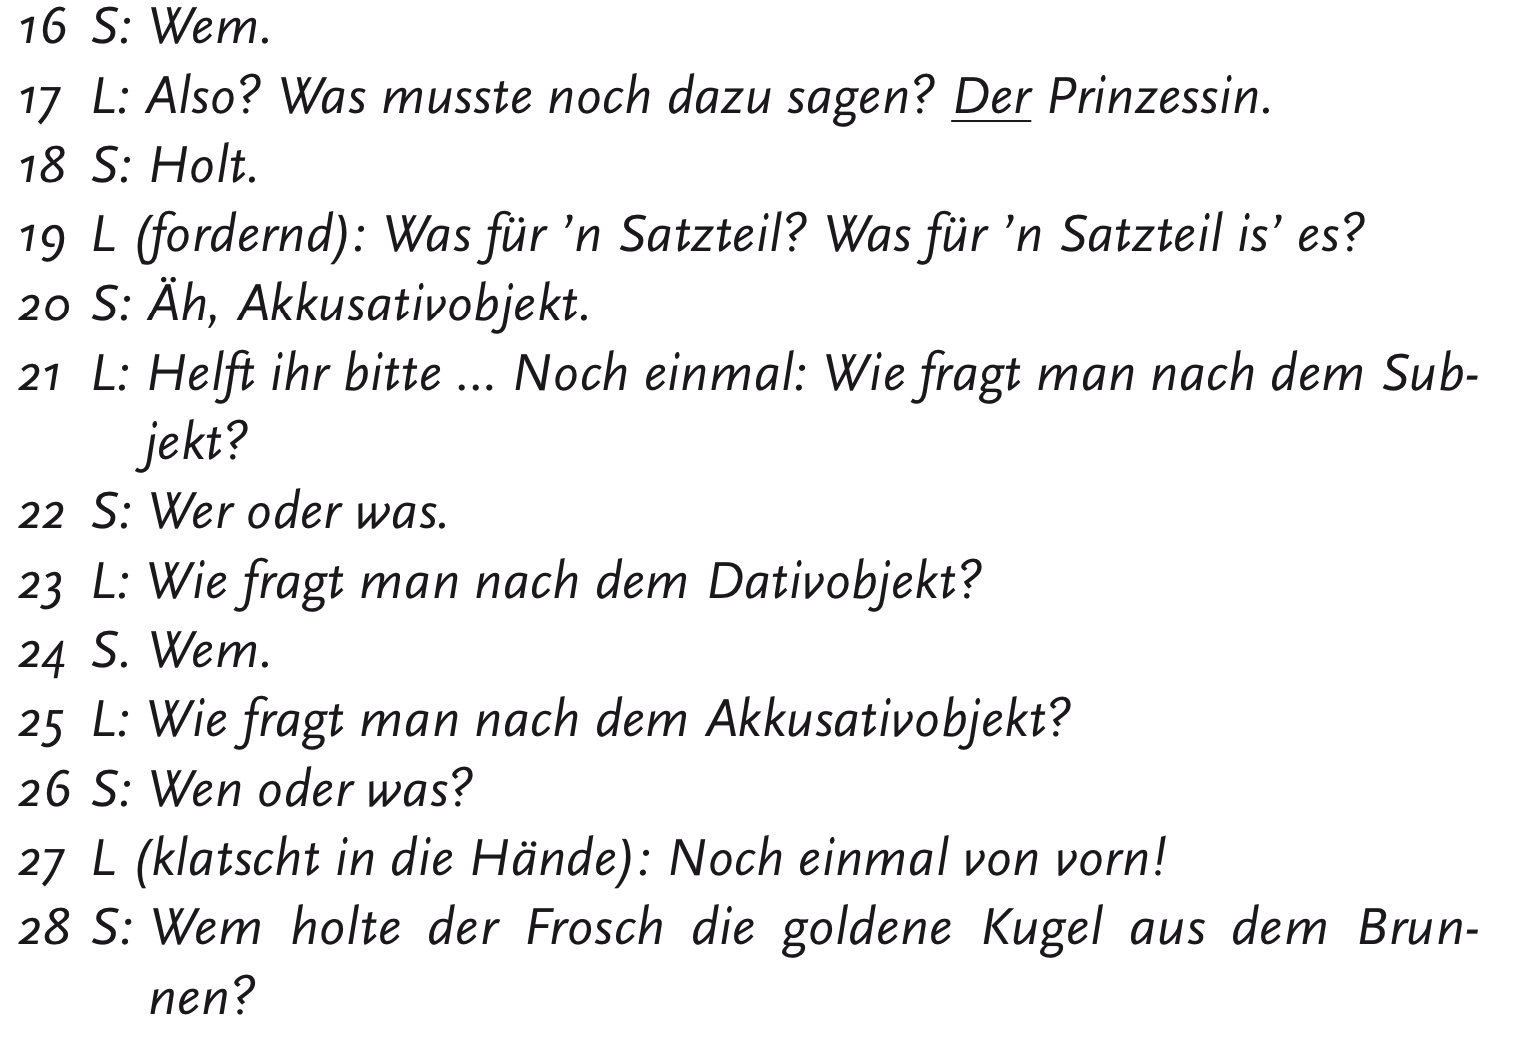
\includegraphics[width=0.6\textwidth]{graphics/kasusschule2}
  \end{center}
  \tiny \citet[36--37]{Gramzowemden2002}, zitiert nach \citet[257--258]{Bredel2013}
\end{frame}

\begin{frame}
  {Morphosyntax in der Schule}
  Wozu ist so ein Unterricht gut?
  \begin{center}
    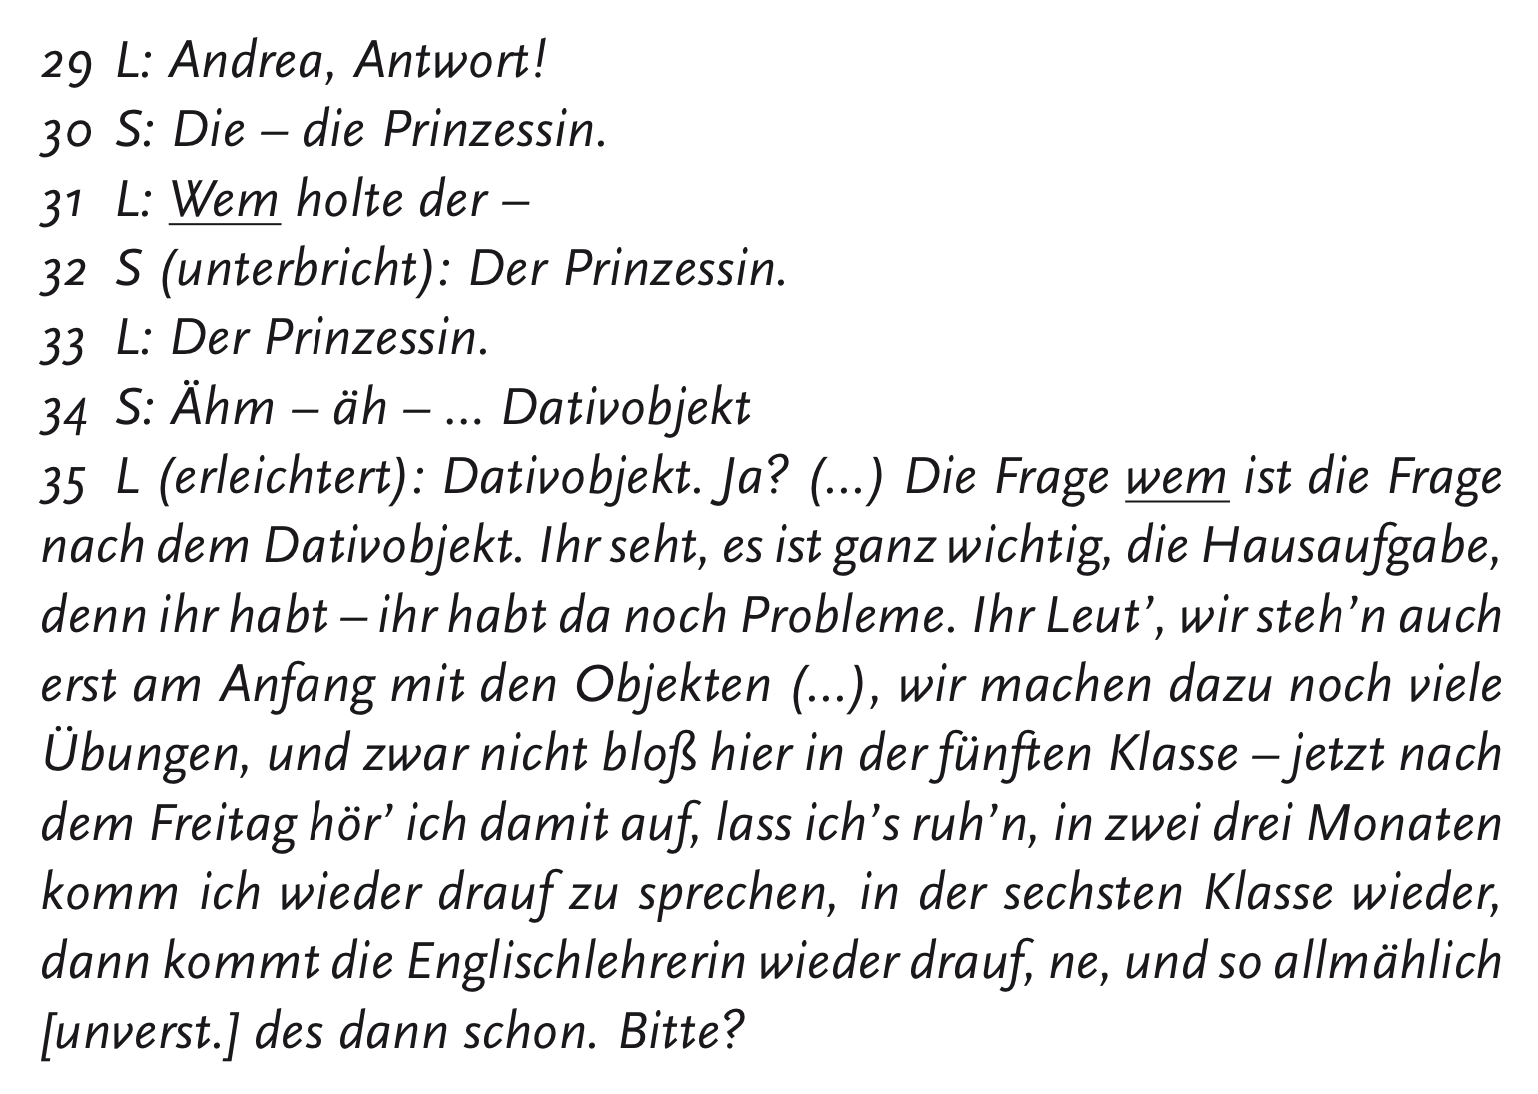
\includegraphics[width=0.6\textwidth]{graphics/kasusschule3}
  \end{center}
  \tiny \citet[36--37]{Gramzowemden2002}, zitiert nach \citet[257--258]{Bredel2013}
\end{frame}

\section{Stämme und Affixe}

\begin{frame}
  {Form und Funktion: Flexion}
  \pause
  \begin{exe}
    \ex
    \begin{xlist}
      \ex \alert{Den Präsidenten} begrüßte \alert{der Dekan} äußerst respektlos.
      \pause
      \ex \alert{Der Dekan} begrüßte \alert{den Präsidenten} äußerst respektlos.
    \end{xlist}
    \pause
    \ex
    \begin{xlist}
      \ex \alert{Die Präsidentin} begrüßte \alert{die Dekanin} äußerst respektlos.
      \pause
      \ex \alert{Die Dekanin} begrüßte \alert{die Präsidentin} äußerst respektlos.
    \end{xlist}
  \end{exe}
  \pause
  \Zeile
  Formveränderungen lexikalischer Wörter \alert{schränken ihre möglichen grammatischen Funktionen und Relationen im Satz ein}\dots\\
  \pause
  \Halbzeile
  \dots und sie haben semantische und systemexterne Folgen.

\end{frame}

\begin{frame}
  {Form und Funktion: Wortbildung}
  \pause
  \begin{exe}
    \ex grün\alert{lich}, röt\alert{lich}, gelb\alert{lich}
    \pause
    \ex Neu\alert{igkeit}, Blöd\alert{heit}, Tauch\alert{er}, Heb\alert{ung}
    \pause
    \ex Fenster\alert{rahmen}, Tücher\alert{spender}, Glas\alert{korken}, Unter\alert{schrank}
  \end{exe}
  \pause
  \Zeile
  Formveränderungen von einem zu einem anderen lexikalischen Wort führen zu Bedeutungs- und kategorialen Veränderungen.
\end{frame}

\begin{frame}
  {Markierungsfunktionen von Morphen I}
  \pause
  \begin{exe}
    \ex
    \begin{xlist}
      \ex{(der) \alert<4>{Berg}}
      \ex{(den) \alert<4>{Berg}}
      \ex{(dem) \alert<4>{Berg}}
      \ex{(des) \alert<5>{Berg}\rot<5>{-es}}
      \ex{(die) \alert<6>{Berg}\rot<6>{-e}}
      \ex{(der) \alert<6>{Berg}\rot<6>{-e}}
    \end{xlist}
    \pause
    \ex
    \begin{xlist}
      \ex{(der) \alert<8>{Mensch}}
      \ex{(den) \alert<9>{Mensch}\rot<9>{-en}}
      \ex{(dem) \alert<9>{Mensch}\rot<9>{-en}}
      \ex{(des) \alert<9>{Mensch}\rot<9>{-en}}
      \ex{(die) \alert<9>{Mensch}\rot<9>{-en}}
      \ex{(der) \alert<9>{Mensch}\rot<9>{-en}}
    \end{xlist}
  \end{exe}
\end{frame}

\begin{frame}
  {Markierungsfunktionen von Morphen II}
  \pause
  \begin{exe}
    \ex
    \begin{xlist}
      \ex{(ich) \alert<3>{kauf}\rot<3>{-e}}
      \ex{(du) \alert<4>{kauf}\rot<4>{-st}}
      \ex{(wir) \alert<5>{kauf}\rot<5>{-en}}
      \ex{(sie) \alert<5>{kauf}\rot<5>{-en}}
    \end{xlist}
  \end{exe}
\end{frame}

\begin{frame}
  {Morphe und Markierungsfunktionen}
  \pause
  \begin{itemize}[<+->]
    \item Formveränderungen:
      \begin{itemize}[<+->]
        \item oft nicht \alert{eine} Funktion
        \item \rot{Einschränkung} der möglichen Funktionen
      \end{itemize}
   \Halbzeile 
    \item \alert{Markierungsfunktion}: eine \alert{Reduktion}\\
      der möglichen Merkmale oder Werte einer Wortform
    \item zum Beispiel \textit{-en} bei schw.\ Maskulina: \rot{nicht} Nominativ Singular
    \item oder \textit{-en} bei Verben im Präsens: Plural und nicht adressatbezogen
      \Halbzeile
    \item \alert{Morphe = alle segmentalen Einheiten mit Markierungsfunktion}
    \item konkret: \alert{Stämme} und \alert{Affixe}
  \end{itemize}
\end{frame}

\begin{frame}
  {Stämme I}
  \pause
  \begin{exe}
    \ex
    \begin{xlist}
      \ex{(ich) \alert<5->{kauf}-e\\
        (du) \alert<5->{kauf}-st\\
        (ihr) \alert<5->{kauf}-t }
        \pause
        \ex{(ich) \alert<6->{kauf}-te\\
        (du) \alert<6->{kauf}-test\\
        (ihr) \alert<6->{kauf}-tet}
        \pause
        \ex{(ich habe) ge-\alert<7->{kauf}-t\\
        (du hast) ge-\alert<7->{kauf}-t\\
        (ihr habt) ge-\alert<7->{kauf}-t}
    \end{xlist}
  \end{exe}
\end{frame}

\begin{frame}
  {Stämme II}
  \begin{exe}
    \ex
    \begin{xlist}
      \ex{(ich) \alert<4->{nehm}-e\\
        (du) \rot<5->{nimm}-st\\
          (es) \rot<5->{nimm}-t\\
          (ihr) \alert<4->{nehm}-t}
        \pause
        \ex{(ich) \orongsch<6->{nahm}\\
        (du) \orongsch<6->{nahm}-st\\
          (ihr) \orongsch<6->{nahm}-t}
        \pause
        \ex{(ich habe) ge-\gruen<7->{nomm}-en\\
        (du hast) ge-\gruen<7->{nomm}-en\\
        (ihr habt) ge-\gruen<7->{nomm}-en}
    \end{xlist}
  \end{exe}
  \pause
  \pause
  \pause
  \pause
  \pause
  Der \alert{Stamm} kann nicht "`der unveränderliche Wortbestandteil"'\\
  eines lexikalischen Wortes (in einem Paradigma) sein.\\
  \Zeile
  \pause
  \alert{\dots aber der mit der Bedeutung, also der lexikalischen Markierungsfunktion}!
\end{frame}

\begin{frame}
  {Affixe}
  \pause
  \begin{exe}
    \ex
    \begin{xlist}
      \ex (ich) nehm\alert<6->{-e}
      \pause
      \ex (des) Berg\alert<7->{-es}
      \pause
      \ex Schön\alert<8->{-heit}
      \pause
      \ex \alert<9->{Un-}ding
    \end{xlist}
  \end{exe}
  \Zeile
  \pause
  \pause
  \pause
  \pause
  \pause
  \begin{itemize}[<+->]
    \item \alert{keine lexikalische Markierungsfunktion} (= keine eigene Bedeutung)
    \item \alert{nicht wortfähig} = nicht ohne Stamm verwendbar
  \end{itemize}
\end{frame}

\section{Umlaut und Ablaut}

\begin{frame}
  {Umlaut vs.\ Ablaut: Warum erst jetzt?}
  \pause
  \alert{"`So ein chaotisches Buch! Plötzlich geht es\\
  in der Morphologie wieder um Phonologie!"'}\pause --- Ja\dots
  \pause
  \Zeile
  \begin{itemize}[<+->]
    \item Morphophonologie
    \item Morphosyntax
    \item Syntax-Semantik-Schnittstelle
    \item Prosodie-Pragmatik-Schnittstelle
    \item usw.
      \Zeile
    \item \rot{Die Grammatik nutzt die verfügbaren Mittel gut aus,\\
      und Markierungsmöglichkeiten aller Ebenen können\\
    auf anderen Ebenen zum Einsatz kommen.}
  \end{itemize}
\end{frame}

\begin{frame}[fragile]
  {Umlaut}
  \pause
  \begin{center}
    \resizebox{0.4\textwidth}{!}{
    \begin{tikzpicture}[scale=3.5,baseline=default]
      \large
      \tikzset{
        vowel/.style={fill=white, anchor=mid, text depth=0ex, text height=1ex},
        vowelgespannt/.style={circle,fill=gray!30, anchor=mid, text depth=0ex, text height=1ex,minimum size=4ex},
        dot/.style={circle,fill=black,minimum size=0.4ex,inner sep=0pt,outer sep=-1pt},
      }

      \coordinate (hf) at (0,2); % high front
      \coordinate (hb) at (2,2); % high back
      \coordinate (lf) at (1,0); % low front
      \coordinate (lb) at (2,0); % low back
      \def\V(#1,#2){barycentric cs:hf={(3-#1)*(2-#2)},hb={(3-#1)*#2},lf={#1*(2-#2)},lb={#1*#2}}

      % Chart key (vorne -- hinten).
      \draw [{Latex[round]}-] (\V (-.25,0)) -- (\V (-.25,.5)) node[above left] {\footnotesize vorne};
      \draw [-{Latex[round]}] (\V (-.25,1.5)) -- (\V (-.25,2)) node[above left] {\footnotesize hinten};
      \path (\V (-.25,1)) node[above] {\footnotesize zentral};

      % Chart key (hoch -- tief).
      \draw [{Latex[round]}-] (\V (0,-.25)) -- +(270:.5cm) node[above right,rotate=90] (vokaltrapez1) {\footnotesize hoch};
      \draw [{Latex[round]}-] (\V (3,-2.5)) -- +(270:-.5cm) node[above left,rotate=90] (vokaltrapez2) {\footnotesize tief};
      \path (\V (1.5,-1)) node[above,rotate=90] {\footnotesize mittel};

      % Grid.
      \draw [gray, thick] (\V(0,0)) -- (\V(0,2));
      \draw [gray, thick] (\V(3,0)) -- (\V(3,2));
      \draw [gray, thick] (\V(0,0)) -- (\V(3,0));
      \draw [gray, thick] (\V(0,2)) -- (\V(3,2));

      % Vowels.
      \path (\V (0,2))     node[vowelgespannt] (u)   {u};
      \path (\V(0,0))      node[vowelgespannt] (y)   {y};
      \path (\V (0.5,1.5)) node[vowel]         (uu)  {ʊ};
      \path (\V(0.5,0.5))  node[vowel]         (yy)  {ʏ};
      \path (\V (1,2))     node[vowelgespannt] (o)   {o};
      \path (\V(1.25,0))   node[vowelgespannt] (oe)  {ø};
      \path (\V(3,1))      node[vowelgespannt] (a)   {a};
      \path (\V(2,0))      node[vowelgespannt] (ee)  {ɛ};
      \path (\V(2.5,1))    node[vowel]         (aa)  {ă};
      \path (\V(1.65,0.5)) node[vowel]         (eee) {ɛ̆};
      \path (\V (1.5,1.4)) node[vowel]         (oo)  {ɔ};
      \path (\V(1.4,0.5))  node[vowel]         (oee) {œ};

      \only<3>{\path (u)  edge [-{Latex[round]}, bend left=10]  (y);}
      \only<4>{\path (uu) edge [-{Latex[round]}, bend left=10]  (yy);}
      \only<5>{\path (o)  edge [-{Latex[round]}, bend right=10] (oe);}
      \only<6>{\path (oo) edge [-{Latex[round]}, bend right=5]  (oee);}
      \only<7>{\path (aa) edge [-{Latex[round]}, bend right=10] (eee);}
      \only<8>{\path (a)  edge [-{Latex[round]}, bend left=10]  (ee);}
      
      \only<9->{\path (u)  edge [-{Latex[round]}, bend left=10]  (y);
        \path (uu) edge [-{Latex[round]}, bend left=10]  (yy);
        \path (o)  edge [-{Latex[round]}, bend right=10] (oe);
        \path (oo) edge [-{Latex[round]}, bend right=5]  (oee);
        \path (aa) edge [-{Latex[round]}, bend right=10] (eee);
        \path (a)  edge [-{Latex[round]}, bend left=10]  (ee);}
    \end{tikzpicture}
    }
  \end{center}
  \raggedleft
  \only<3>{G\rot{u}t [g\rot{uː}t] -- G\rot{ü}ter [g\rot{yː}tɐ]\AbUmlautBreaker}
  \only<4>{M\rot{u}tter [m\rot{ʊ}tɐ] -- M\rot{ü}tter [m\rot{ʏ}tɐ]\AbUmlautBreaker}
  \only<5>{T\rot{o}n [t\rot{oː}n]-- T\rot{ö}ne [t\rot{øː}nə]\AbUmlautBreaker}
  \only<6>{\rot{o}ft [ʔ\rot{ɔ}ft] -- \rot{ö}fter [ʔ\rot{œ}ftɐ]\AbUmlautBreaker}
  \only<7>{kr\rot{a}nk [kʁ\rot{a}ŋk] -- kr\rot{ä}nker [kʁ\rot{ɛ}ŋkɐ]\AbUmlautBreaker}
  \only<8>{B\rot{a}d [b\rot{aː}t] -- B\rot{ä}der [b\rot{ɛ}dɐ]}
  \ifdefined\HANDOUT
    \newline
  \fi
  \onslide<9->{Ein vorhersagbarer Prozess: \alert{Frontierung!}}
\end{frame}

\begin{frame}[fragile]
  {Vokalstufen (überwiegend Ablaut)}
  \pause
  Eine kleine Auswahl der möglichen Reihen von Vokalstufen\ldots
  \pause
  \begin{center}
    \resizebox{0.4\textwidth}{!}{
    \begin{tikzpicture}[scale=3.5,baseline=default]
      \large
      \tikzset{
        vowel/.style={fill=white, anchor=mid, text depth=0ex, text height=1ex},
        dot/.style={circle,fill=black,minimum size=0.4ex,inner sep=0pt,outer sep=-1pt},
      }

      \coordinate (hf) at (0,2); % high front
      \coordinate (hb) at (2,2); % high back
      \coordinate (lf) at (1,0); % low front
      \coordinate (lb) at (2,0); % low back
      \def\V(#1,#2){barycentric cs:hf={(3-#1)*(2-#2)},hb={(3-#1)*#2},lf={#1*(2-#2)},lb={#1*#2}}

      % Chart key (vorne -- hinten).
      \draw [{Latex[round]}-] (\V (-.25,0))   -- (\V (-.25,.5)) node [above left] {\footnotesize vorne};
      \draw [-{Latex[round]}] (\V (-.25,1.5)) -- (\V (-.25,2))  node [above left] {\footnotesize hinten};
      \path (\V (-.25,1)) node[above] {\footnotesize zentral};

      % Chart key (hoch--tief).
      \draw [{Latex[round]}-] (\V (0,-.25)) -- +(270:.5cm)  node [above right,rotate=90] (vokaltrapez1) {\footnotesize hoch};
      \draw [{Latex[round]}-] (\V (3,-2.5)) -- +(270:-.5cm) node [above left,rotate=90] (vokaltrapez2) {\footnotesize tief};
      \path (\V (1.5,-1)) node[above,rotate=90] {\footnotesize mittel};

      % Grid. 
      \draw [gray, thick] (\V(0,0)) -- (\V(0,2));
      \draw [gray, thick] (\V(1,0)) -- (\V(1,2));
      \draw [gray, thick] (\V(2,0)) -- (\V(2,2));
      \draw [gray, thick] (\V(3,0)) -- (\V(3,2));
      \draw [gray, thick] (\V(0,0)) -- (\V(3,0));
      \draw [gray, thick] (\V(0,1)) -- (\V(3,1));
      \draw [gray, thick] (\V(0,2)) -- (\V(3,2));

      % Unrounded-rounded pairs.
      \path (\V(0,0))     node [vowel] (i)   {i};
      \path (\V(0.5,0.5)) node [vowel] (I)   {ɪ};   
      \path (\V(1,0))     node [vowel] (e)   {e};
      \path (\V(2,0))     node [vowel] (E)   {ɛ};

      % Unpaired symbols.
      \path (\V(3,1))      node [vowel] (a)  {a};
      \path (\V (2,2))     node [vowel] (oo) {ɔ};
      \path (\V (1,2))     node [vowel] (o)  {o};
      \path (\V (0,2))     node [vowel] (u)  {u};
      \path (\V (0.5,1.5)) node [vowel] (uu) {ʊ};

      \only<4>{\path (i)  edge [red, *-{Latex[round, width=5pt]}, bend left=10] (o);}
      \only<5>{\path (e)  edge [cyan, *-{Latex[round, width=5pt]}, bend left=10] (o);}
      \only<6>{\path (I)  edge [blue, *-, bend right=10] (a);\path (a)  edge [blue, -{Latex[round, width=5pt]}, bend right=10] (uu);}
      \only<7>{\path (E)  edge [green, *-{Latex[round, width=5pt]}, bend right=10] (a);\path (a)  edge [green, -{Latex[round, width=5pt]}, bend right=10] (oo);}
      \only<8>{\path (a)  edge [brown, *-, bend right=10] (u);\path (u)  edge [brown, -{Latex[round, width=5pt]}, bend right=10] (a);}
      \only<9>{\path (u)  edge [orange, *-, bend right=10] (i);\path (i)  edge [orange, -{Latex[round, width=5pt]}, bend right=10] (u);}
      \only<10>{\path (I)  edge [purple, *-, bend left=10] (a);\path (a)  edge [purple, -{Latex[round, width=5pt]}, bend right=10] (E);}

      \only<11>{\path (i)  edge [red, *-{Latex[round, width=5pt]}, bend left=10] (o);
        \path (e)  edge [cyan, *-{Latex[round, width=5pt]}, bend left=10] (o);
        \path (I)  edge [blue, *-, bend right=10] (a);\path (a)  edge [blue, -{Latex[round, width=5pt]}, bend right=10] (uu);
        \path (E)  edge [green, *-{Latex[round, width=5pt]}, bend right=10] (a);\path (a)  edge [green, -{Latex[round, width=5pt]}, bend right=10] (oo);
        \path (a)  edge [brown, *-, bend right=10] (u);\path (u)  edge [brown, -{Latex[round, width=5pt]}, bend right=10] (a);
        \path (u)  edge [orange, *-, bend right=10] (i);\path (i)  edge [orange, -{Latex[round, width=5pt]}, bend right=10] (u);
        \path (I)  edge [purple, *-, bend left=10] (a);\path (a)  edge [purple, -{Latex[round, width=5pt]}, bend right=10] (E);}


    \end{tikzpicture}
    }
  \end{center}
  \raggedleft
  \ifdefined\HANDOUT
    \tiny
  \fi
  \only<4>{fr\textcolor{red}{ie}ren [fʁ\textcolor{red}{iː}ʁən] -- fr\textcolor{red}{o}r [fr\textcolor{red}{oː}͡ɐ] -- gefr\textcolor{red}{o}ren [gəfr\textcolor{red}{oː}ʁən]\AbUmlautBreaker}
  \only<5>{h\textcolor{cyan}{e}ben [h\textcolor{cyan}{eː}bən] -- h\textcolor{cyan}{o}b [h\textcolor{cyan}{oː}p] -- geh\textcolor{cyan}{o}ben [gəh\textcolor{cyan}{oː}bən]\AbUmlautBreaker}
  \only<6>{b\textcolor{blue}{i}nden [b\textcolor{blue}{ɪ}ndən] -- b\textcolor{blue}{a}nd [b\textcolor{blue}{a}nt] -- geb\textcolor{blue}{u}nden [gəb\textcolor{blue}{ʊ}ndən]\AbUmlautBreaker}
  \only<7>{b\textcolor{green}{e}rgen [b\textcolor{green}{ɛ}͡əgən] -- b\textcolor{green}{a}rg [b\textcolor{green}{a}͡ək] -- geb\textcolor{green}{o}rgen [gəb\textcolor{green}{ɔ}͡əgən]\AbUmlautBreaker}
  \only<8>{sch\textcolor{brown}{a}ffen [ʃ\textcolor{brown}{a}fən] -- sch\textcolor{brown}{u}f [ʃ\textcolor{brown}{uː}f] -- gesch\textcolor{brown}{a}ffen [gəʃ\textcolor{brown}{a}fən]\AbUmlautBreaker}
  \only<9>{sch\textcolor{orange}{i}nden [ʃ\textcolor{orange}{ɪ}ndən] -- sch\textcolor{orange}{u}nd [ʃ\textcolor{orange}{ʊ}nt] -- gesch\textcolor{orange}{u}nden [gəʃ\textcolor{orange}{ʊ}ndən]\AbUmlautBreaker}
  \only<10>{s\textcolor{purple}{i}tzen [z\textcolor{purple}{ɪ}t͡sən] -- s\textcolor{purple}{a}ß [z\textcolor{purple}{aː}s] -- ges\textcolor{purple}{e}ssen [gəz\textcolor{purple}{ɛ}sən]}
  \ifdefined\HANDOUT
    \newline
  \fi
  \onslide<11->{\rot{Kein vorhersagbarer Prozess!} Lexikalisch\slash verbklassenbasiert.}
\end{frame}

\section{Merkmale in Flexion und Wortbildung}

\begin{frame}
  {Statische und volatile Merkmale}
  \pause
  \begin{itemize}[<+->]
    \item Eigenschaften: "`Rotsein"' (Erdbeere), "`325m hoch"' (Eiffelturm) usw.
    \item Merkmale: \alert{\textsc{Farbe}}, \alert{\textsc{Länge}} usw.
    \item Werte:
      \begin{itemize}[<+->]
        \item \alert{\textsc{Farbe}}: \rot{\textit{rot}}, \rot{\textit{grau}}, \ldots
        \item \alert{\textsc{Länge}}: \rot{\textit{3cm}}, \rot{\textit{325m}}, \ldots
      \end{itemize}
  \end{itemize}
  \pause
  \Halbzeile 
  \begin{exe}
    \ex
    \begin{xlist}
      \ex{Haus = [\textsc{Bed}: \gruen<12->{\textbf{\textit{haus}}}, \textsc{Klasse}: \gruen<12->{\textbf{\textit{subst}}}, \textsc{Gen}: \gruen<12->{\textbf{\textit{neut}}}, \textsc{Kas}: \orongsch<13->{\textit{nom}}, \textsc{Num}: \orongsch<13->{\textit{sg}}]}
      \pause
      \ex{Haus-es = [\textsc{Bed}: \gruen<12->{\textbf{\textit{haus}}}, \textsc{Klasse}: \gruen<12->{\textbf{\textit{subst}}}, \textsc{Gen}: \gruen<12->{\textbf{\textit{neut}}}, \textsc{Kas}: \orongsch<13->{\textit{gen}}, \textsc{Num}: \orongsch<13->{\textit{sg}}]}
      \pause
      \ex{Häus-er = [\textsc{Bed}: \gruen<12->{\textbf{\textit{haus}}}, \textsc{Klasse}: \gruen<12->{\textbf{\textit{subst}}}, \textsc{Gen}: \gruen<12->{\textbf{\textit{neut}}}, \textsc{Kas}: \orongsch<13->{\textit{nom}}, \textsc{Num}: \orongsch<13->{\textit{pl}}]}
    \end{xlist}
  \end{exe}
  \Halbzeile
  \pause
  \begin{itemize}[<+->]
    \item bei einem lexikalischen Wort:
      \begin{itemize}
        \item \gruen{statische Merkmale} wertestabil
        \item \orongsch{volatile Merkmale} werteverändernd im Paradigma
      \end{itemize}
  \end{itemize}
\end{frame}

\begin{frame}
  {Wortbildung in Abgrenzung zur Flexion}
  \pause
  \begin{exe}
    \ex
    \begin{xlist}
      \ex trocken (Adj) → \alert{Trocken}\rot{-heit} (Subst)
      \ex Kauf (Subst), Rausch (Subst) → \alert{Kauf}\rot{-rausch} (Subst)
      \ex gehen (V) → \alert{be}\rot{-gehen} (V)
    \end{xlist}
    \pause
    \ex
    \begin{xlist}
      \ex \alert{lauf}\rot{-en} (1\slash 3 Pl Prs Ind) → \alert{lauf}\rot{-e} (1 Sg Prs Ind)
      \ex \alert{Münze} (Sg) → \alert{Münze}\rot{-n} (Pl)
    \end{xlist}
  \end{exe}
  \pause
  \Halbzeile
  \begin{itemize}[<+->]
    \item Wortbildung
      \begin{itemize}[<+->]
        \item statische Merkmale geändert (Wortklasse, Bedeutung)
        \item \ldots oder gelöscht (alles außer Bedeutung: Erstglied bei Komposition)
        \item \ldots oder umgebaut (Valenz von Verben beim Applikativ)
        \item \alert{produktives Erschaffen neuer lexikalischer Wörter}
      \end{itemize}
  \Halbzeile
    \item Flexion
      \begin{itemize}
        \item Änderung der Werte volatiler Merkmale
        \item typisch: Anpassung an syntaktischen Kontext
      \end{itemize}
  \end{itemize}
\end{frame}

\section{Funktion in der Flexion}

\subsection{Nominalflexion}

\begin{frame}
  {Was heißt Funktion?}
  \pause
  Rückgriff auf Kapitel 3:
  \pause
  \Halbzeile
  \begin{itemize}[<+->]
    \item \alert{externe} Funktion: kommunikativ, pragmatisch, textuell, kulturell, \dots
    \item \alert{interne} Funktion: innerhalb der Grammatik Relationen kennzeichnend,
      Rekonstruktion der Struktur ermöglichend, Schnittstelle zur Semantik: \rot{Kompositionalität}
    \item nicht immer trennbar
      \Halbzeile
    \item Paradebeispiel für interne Funktion: \alert{Kasussystem}
  \end{itemize}
\end{frame}

\begin{frame}
  {Numerus}
  \pause
  \begin{exe}
    \ex
    \begin{xlist}
      \ex[ ]{Die Trainerin beobachtet [einen guten Wettkampf].}
      \pause
      \ex[*]{Die Trainerin beobachtet [einen guten \rot{Wettkämpfe}].}
    \end{xlist}
    \pause
    \ex
    \begin{xlist}
      \ex[ ]{Die Trainerin beobachtet [einige gute Wettkämpfe].}
      \pause
      \ex[*]{Die Trainerin beobachtet [einige gute \rot{Wettkampf}].}
    \end{xlist}
  \end{exe}
  \pause
  \Halbzeile
  \begin{itemize}[<+->]
    \item \alert{Anzahl von Objekten ("`Gegenständen"')}: konzeptuell beim Subst motiviert
    \item notwendigerweise volatiles Merkmal beim Subst
    \item Pluraliatantum wie \textit{Ferien} oder Singulariatantum wie \textit{Gesundheit}
  \end{itemize}
\end{frame}

\begin{frame}
  {Kasus}
  \pause
  Was ist Kasus? Haben die Kasus an sich eine Bedeutung?
  \Halbzeile
  \pause
  \begin{exe}
    \ex
    \begin{xlist}
      \ex{Wir sehen \rot{den Rasen}.}
      \pause
      \ex{Wir begehen \rot{den Rasen}.}
      \pause
      \ex{Wir säen \rot{den Rasen}.}
      \pause
      \ex{Wir fürchten \rot{uns}.}
    \end{xlist}
    \pause
    \ex
    \begin{xlist}
      \ex \rot{Nächsten März} fahre ich zum Bergwandern in die Tatra.
      \ex Es waren \rot{den ganzen Tag} Menschen zum Gipfel unterwegs.
    \end{xlist}
    \pause
    \ex
    \begin{xlist}
      \ex{Sarah backt \rot{ihrer Freundin} einen Marmorkuchen.}
      \pause
      \ex{Wir kaufen \rot{dir} ein Kilo Rohrzucker.}
      \pause
      \ex{Die Mannschaft spielt \rot{mir} zu drucklos.}
      \pause
      \ex{Der Marmorkuchen schmeckt \rot{den Freundinnen} gut.}
    \end{xlist}
  \end{exe}
\end{frame}


\begin{frame}
  {Kasus: Eigenschaften}
  \pause
  \centering

  \Large Kasus stellt Relationen zwischen Nomina und anderen Wörtern (\zB\ Verben, Präpositionen, anderen Nomina) her.\\
\end{frame}

\begin{frame}
  {Person: Deixis}
  \pause
  Was ist die grammatische Person?

  \Halbzeile
  \pause
  \begin{exe}
    \ex
    \begin{xlist}
      \ex{\alert{Ich} unterstütze den FCR Duisburg.}
      \pause
      \ex{\alert{Ihr} unterstützt den FCR Duisburg.}
      \pause
      \ex{\alert{Sie/Diese/Jene/Eine/Man\ldots} unterstützt den FCR Duisburg.}
      \pause
      \ex{\alert{Sie/Diese/Jene/Einige/\ldots} unterstützen den FCR Duisburg.}
    \end{xlist}
  \end{exe}
  \pause
  \Halbzeile
  \begin{itemize}[<+->]
    \item prototypisch beim \alert{Pronomen} funktional motiviert
    \item Substantive: statisch dritte Person
      \Halbzeile
    \item hier: \rot{deiktische Pronomina}
      \begin{itemize}[<+->]
        \item in einer Situation verweisend
        \item nur relativ zu einer Situation interpretierbar
      \end{itemize} 
  \end{itemize}
\end{frame}

\begin{frame}
  {Person: Anaphorik}
  \pause
  \begin{exe}
    \ex \alert{Sarah$_{\textnormal{1}}$} backt \rot{[ihrer Freundin]$_{\textnormal{2}}$} \gruen{[einen Kuchen]$_{\textnormal{3}}$}.\\
      \alert{Sie$_{\textnormal{1}}$} verwendet nur fair gehandelten unraffinierten Rohrzucker.
    \pause
      \ex \alert{Sarah$_{\textnormal{1}}$} backt \rot{[ihrer Freundin]$_{\textnormal{2}}$} \gruen{[einen Kuchen]$_{\textnormal{3}}$}.\\
      \gruen{Er$_{\textnormal{3}}$} besteht nur aus fair gehandelten Zutaten.
    \pause
      \ex \alert{Sarah$_{\textnormal{1}}$} backt \rot{[ihrer Freundin]$_{\textnormal{2}}$} \gruen{[einen Kuchen]$_{\textnormal{3}}$}.\\
      \rot{Sie$_{\textnormal{2}}$} soll \gruen{ihn$_{\textnormal{3}}$} zum Geburtstag geschenkt bekommen.
  \end{exe}
  \Halbzeile
  \pause
  \begin{itemize}[<+->]
    \item anaphorische Pronomina
    \item Rückverweis im Text, Satz, Diskurs
    \item gleiche Indizes zeigen Bedeutungsidentität: Korreferenz
  \end{itemize}
\end{frame}

\begin{frame}
  {Genus, Geschlecht, Gender?}
  \pause
  \begin{exe}
    \ex \label{ex:genus039}
    \begin{xlist}
      \ex \alert{Die Petunie} ist \orongsch{eine Blume}.
      \ex \rot{Der Enzian} ist \orongsch{eine Blume}.
      \ex \gruen{Das Veilchen} ist \orongsch{eine Blume}.
    \end{xlist}
  \end{exe}
  \pause
  \Halbzeile
  \begin{itemize}[<+->]
    \item reine Subklassenbildung beim Substantiv
    \item nicht in Geschlecht oder Gender motiviert
    \item tendentiell Korrespondenz von maskulin und männlich\\
      sowie feminin und weiblich bei Menschen bzw.\ Lebewesen
  \end{itemize}
\end{frame}

\subsection{Verbalflexion}

\begin{frame}
  {Numerus und Person bei Verben}
  \pause
  \begin{itemize}[<+->]
    \item wie gezeigt wurde: \alert{Numerus} und \alert{Person}\\
      im Bereich der Nomina motiviert
    \item Numerus und Person bei Verben: Subjekt-Verb-Kongruenz 
      \Halbzeile
    \item Kongruenz:
      \begin{itemize}[<+->]
        \item reine \alert{Übereinstimmung von Werten}
        \item \rot{beide Einheiten} haben das Merkmal
        \item \alert{Kongruenz zwischen Nomina}: \textit{der schöne Kaftan}
        \item \alert{Subjekt-Verb-Kongruenz}: \textit{Ich schwafle.}
      \end{itemize}
  \end{itemize}
\end{frame}

\begin{frame}
  {Tempus: synthetisch vs.\ analytisch}
  \pause
  Die klassischen "`Tempusformen"' des Deutschen:\\
  \Halbzeile
  \pause
  \begin{center}
    \scalebox{0.75}{\begin{tabular}{ll}
      \toprule
      \textbf{Tempus} & \textbf{Beispiel 3.~Person}\\
      \midrule
      Präsens & \alert<4->{lacht} \\
      Präteritum & \alert<4->{lachte} \\
      Perfekt & hat gelacht \\
      Plusquamperfekt & hatte gelacht \\
      Futur & wird lachen \\
      Futurperfekt & wird gelacht haben \\
      \bottomrule
    \end{tabular}}
  \end{center}
  \pause
  \Halbzeile
  \begin{itemize}[<+->]
    \item \alert{Ganz offensichtlich hat das Deutsche nur zwei Tempusformen\\
      im morphologischen Sinn.}
  \end{itemize} 
\end{frame}

\begin{frame}
  {Funktion: einfache Tempora}
  \pause
  \alert{Präsens: Ereignis- und Sprechzeitpunkt unabhängig}
  \pause
  \begin{exe}\ex\begin{xlist}
      \ex Im Jahr 1961 \alert{beginnt} die DDR mit dem Bau der Mauer.
      \pause
      \ex Morgen \alert{esse} ich Maronen.
      \pause
      \ex Heute \alert{ist} Mittwoch, und donnerstags \alert{kommt} die Müllabfuhr.
  \end{xlist}\end{exe}
  \pause
  \Halbzeile
  \alert{Präteritum: Ereignis- vor Sprechzeitpunkt}
  \pause
  \begin{exe}\ex\begin{xlist}
      \ex Es \alert{klingelte} an der Tür.
      \pause
    \ex Jetzt \alert{klingelte} es an der Tür.
      \pause
    \ex Die Hethiter \alert{wurden} aus Anatolien vertrieben.
  \end{xlist}\end{exe}
  \pause
  \Halbzeile
  \alert{Futur: Ereignis- vor Sprechzeitpunkt}
  \pause
  \begin{exe}\ex\begin{xlist}
      \ex Ich \alert{werde} einen Rottweiler \alert{adoptieren}.
      \pause
      \ex Viele Verstärker \rot{werden} von mir noch \alert{repariert} \rot{werden}.
  \end{xlist}\end{exe}
\end{frame}

\begin{frame}
  {Funktion: komplexe Tempora}
  \pause
  Zusätzlicher Bezug auf einen Referenzzeitpunkt!\\
  \Zeile
  \pause
  \alert{Futurperfekt: Sprech- und Ereigniszeit vor Referenzzeit}
  \pause
  \begin{exe}
    \ex In zwei Jahren \alert{wird} Merkel \alert{abgedankt haben}.
    \pause
    \ex Im Jahr 2010 \alert{wird} Helmut Schmidt \alert{abgedankt haben}.
  \end{exe}
  \pause
  \Zeile
  \alert{Plusquamperfekt: Referenz- vor Sprechzeit, Ereignis- vor Referenzzeit}
  \pause
  \begin{exe}
    \ex Frida nahm das Buch in die Hand. Sie \alert{hatte} es bereits \alert{gelesen}.
      \pause
    \ex Frida legte das Buch weg, nachdem sie es \alert{gelesen hatte}.
  \end{exe}
\end{frame}

\begin{frame}
  {Modus: Grade der Faktizität}
  \pause
  \alert{Indikativ}, \orongsch{Konjunktiv I}, \rot{Konjunktiv II}:
  \pause
  \small
  \begin{exe}
    \ex
    \begin{xlist}
      \ex[]{Sie sagte, der Kuchen \alert{schmeckt} lecker.}
      \ex[]{Sie sagte, der Kuchen \orongsch{schmecke} lecker.}
      \ex[]{Sie sagte, dass der Kuchen lecker \alert{schmeckt}.}
      \ex[]{Sie sagte, dass der Kuchen lecker \orongsch{schmecke}.}
    \end{xlist}
    \pause
    \ex
    \begin{xlist}
      \ex[]{Wenn das \alert{geschieht}, \alert{laufe} ich weg.}
      \ex[]{Immer, wenn das \alert{geschieht}, \alert{laufe} ich weg.}
      \ex[]{Wenn das \rot{geschähe}, \rot{liefe} ich weg.}
      \ex[*]{Immer, wenn das \rot{geschähe}, \rot{liefe} ich weg.}
    \end{xlist}
    \pause
    \ex
    \begin{xlist}
      \ex[]{Ohne Schnee \alert{sind} die Ferien diesmal nicht so schön.}
      \ex[]{Ohne Schnee \rot{wären} die Ferien diesmal nicht so schön.}
    \end{xlist}
    \pause
    \ex
    \begin{xlist}
      \ex[]{Im Urlaub \alert{hat} kein Schnee gelegen.}
      \ex[]{Ach, \rot{hätte} im Urlaub doch Schnee gelegen.}
    \end{xlist}
  \end{exe}
\end{frame}

\begin{frame}
  {Warum gehört Genus Verbi hier nicht hin?}
  \pause
  \begin{exe}
    \ex
    \begin{xlist}
      \ex \rot{Frida} \alert{isst} \orongsch{den Kuchen}.
      \pause
      \ex \orongsch{Der Kuchen} \alert{wird} \alert{gegessen}.
      \pause
      \ex \orongsch{Der Kuchen} \alert{wird} \rot{von Frida} \alert{gegessen}.
    \end{xlist}
  \end{exe}
  \pause
  \Zeile
  \begin{itemize}[<+->]
    \item \rot{keine Flexion} (wie analytische Tempora)
    \item eigentlich eine \alert{lexikalische} Änderung am Verb\\
      (Valenzänderung und Partizipform, s.\ ca.\ Woche 11)
  \end{itemize}
\end{frame}

\section{Vorschau}

\begin{frame}
  {Wortbildung}
  \pause
  \begin{itemize}[<+->]
    \item Wortbildung stellt einen unbegrenzten Wortschatz sicher.
    \item Im Deutschen hängt ein Großteil der Audrucksfähigkeit\\
      komplexer Sachverhalte an der Wortbildung.
      \Zeile
    \item Komposition: \textit{Schulheft}, \textit{linksrheinisch} usw.
    \item Konversion: \textit{der Lauf}, \textit{das Gehen} usw.
    \item Derivation: \textit{Klavierchen}, \textit{erkennbar}, \textit{Verehrung}, \textit{Wasserspringerin} usw.
  \end{itemize}
  \pause
  \begin{center}
    Bitte lesen Sie bis nächste Woche: \alert{Kapitel 8, S.~221--245}
  \end{center}
\end{frame}


  \documentclass[handout,aspectratio=1610]{beamer}
%\documentclass[aspectratio=1610]{beamer}

%\usepackage[T1]{fontenc}
\usepackage[ngerman]{babel}
\usepackage{color}
\usepackage{colortbl}
\usepackage{textcomp}
\usepackage{multirow}
\usepackage{nicefrac}
\usepackage{multicol}
\usepackage{gb4e-}
\usepackage{verbatim}
\usepackage{cancel}
\usepackage{graphicx}
\usepackage{hyperref}
\usepackage{verbatim}
\usepackage{boxedminipage}
\usepackage{rotating}
\usepackage{booktabs}
\usepackage{bbding}

\usepackage{tikz}
\usetikzlibrary{positioning,arrows,cd}
\tikzset{>=latex}

\usepackage[linguistics]{forest}

\usepackage{FiraSans}

\usepackage[maxbibnames=99,
  maxcitenames=2,
  uniquelist=false,
  backend=biber,
  doi=false,
  url=false,
  isbn=false,
  bibstyle=biblatex-sp-unified,
  citestyle=sp-authoryear-comp]{biblatex}
\addbibresource{rs.bib}

\forestset{
  Ephr/.style={draw, ellipse, thick, inner sep=2pt},
  Eobl/.style={draw, rounded corners, inner sep=5pt},
  Eopt/.style={draw, rounded corners, densely dashed, inner sep=5pt},
  Erec/.style={draw, rounded corners, double, inner sep=5pt},
  Eoptrec/.style={draw, rounded corners, densely dashed, double, inner sep=5pt},
  Ehd/.style={rounded corners, fill=gray, inner sep=5pt,
    delay={content=\whyte{##1}}
  },
  Emult/.style={for children={no edge}, for tree={l sep=0pt}},
  phrasenschema/.style={for tree={l sep=2em, s sep=2em}},
  decide/.style={draw, chamfered rectangle, inner sep=2pt},
  finall/.style={rounded corners, fill=gray, text=white},
  intrme/.style={draw, rounded corners},
  yes/.style={edge label={node[near end, above, sloped, font=\scriptsize]{Ja}}},
  no/.style={edge label={node[near end, above, sloped, font=\scriptsize]{Nein}}},
  sake/.style={tier=preterminal},
  ake/.style={
    tier=preterminal
    },
}


\tikzset{
    invisible/.style={opacity=0,text opacity=0},
    visible on/.style={alt=#1{}{invisible}},
    alt/.code args={<#1>#2#3}{%
      \alt<#1>{\pgfkeysalso{#2}}{\pgfkeysalso{#3}} % \pgfkeysalso doesn't change the path
    },
}
\forestset{
  visible on/.style={
    for tree={
      /tikz/visible on={#1},
      edge+={/tikz/visible on={#1}}}}}

\definecolor{lg}{rgb}{.8,.8,.8}
\newcommand{\Dim}{\cellcolor{lg}}


\newcommand{\Sub}[1]{\ensuremath{_{\text{#1}}}}
\newcommand{\Up}[1]{\ensuremath{^{\text{#1}}}}

\newcommand{\Ck}{\CheckmarkBold}
\newcommand{\Fl}{\XSolidBrush}

\usetheme[hideothersubsections]{Goettingen}

%\newcommand{\rot}[1]{{\color[rgb]{0.4,0.2,0}#1}}
%\newcommand{\blau}[1]{{\color[rgb]{0,0,.9} #1}}
\newcommand{\gruen}[1]{{\color[rgb]{0,0.4,0}#1}}

\newcommand{\rot}[1]{{\color[rgb]{0.6,0.2,0.0}#1}}
\newcommand{\blau}[1]{{\color[rgb]{0.0,0.0,0.9}#1}}
\newcommand{\orongsch}[1]{{\color[RGB]{255,165,0}#1}}
\newcommand{\grau}[1]{{\color[rgb]{0.5,0.5,0.5}#1}}

\renewcommand<>{\rot}[1]{%
  \alt#2{\beameroriginal{\rot}{#1}}{#1}%
}
\renewcommand<>{\blau}[1]{%
  \alt#2{\beameroriginal{\blau}{#1}}{#1}%
}
\renewcommand<>{\orongsch}[1]{%
  \alt#2{\beameroriginal{\orongsch}{#1}}{#1}%
}

\definecolor{trueblue}{rgb}{0,0.0,0.7}
\setbeamercolor{alerted text}{fg=trueblue}

\newcommand{\xxx}{\hspaceThis{[}}
\newcommand{\zB}{z.\,B.\ }
\newcommand{\down}[1]{\ensuremath{\mathrm{#1}}}

\newcommand{\Zeile}{\vspace{\baselineskip}}
\newcommand{\Halbzeile}{\vspace{0.5\baselineskip}}
\newcommand{\Viertelzeile}{\vspace{0.25\baselineskip}}

\resetcounteronoverlays{exx}

\title{Einführung in die Sprachwissenschaft\\
7.~Wortbildung}
\author{Roland Schäfer}
\institute{Deutsche und niederländische Philologie\\Freie Universität Berlin}
\date{Wintersemester 2018/2019\\11.~Dezember 2018}

\begin{document}

\frame{\titlepage}

\section{Vorab}

\begin{frame}
  {Schreib- und Schriftunterricht}
  \pause
  \begin{itemize}[<+->]
    \item Berliner Schulen (zumindest einige; und wer weiß wo sonst noch):
      \begin{itemize}[<+->]
        \item Kinder sollen in der ersten und zweiten Klasse\\
          erstmal schreiben, wie sie sprechen.
        \item \alert{"`Sehr gut! Aber Erwachsene würden das anders schreiben."'}
      \end{itemize}
      \Halbzeile
    \item schlimmer als die klassische \alert{Hinhörschreibung}:\\
      \rot{\textbf{Hinhörschreibung\slash Sprechschreibung ohne Anleitung\slash Steuerung}}
      \Halbzeile
    \item \rot{ohne jede Fundierung in Lerntheorien}
    \item \rot{kann zu erheblichen permanenten Rechtschreibschwächen führen}
    \item \rot{\textbf{Machen Sie so einen Schwachsinn nicht mit!}}
    \Halbzeile
    \item Natürlich "`lernen es die meisten \rot{trotzdem}"' (durch Lesen),\\
      aber ebenso natürlich gibt es selbst \rot{unter Ihnen} immer noch\\
      Personen mit erheblichen Mängeln in Orthographie, Interpunktion und\\
      bildungssprachlichen Kompetenzen!
    \item \alert{Das muss} \rot{für alle} \alert{vermieden werden.}
  \end{itemize}
\end{frame}

\section{Rückblick}

\begin{frame}
  {Wortbildung und Flexion}
  \pause
  \begin{itemize}[<+->]
    \item Flexion als Mittel zur Dekodierung von (syntaktischer) Struktur
    \item Wortbildung als Mittel der Wortschatzerweiterung und -optimierung
      \Zeile
    \item Markierungsfunktion von Morphen:\\
      \alert{Einschränkung} der möglichen Funktion
    \item Stämme: mit lexikalischer Markierungsfunktion
    \item Affixe: ohne lexikalische Markierungsfunktion; nicht wortfähig
      \Zeile
    \item Umlaut: (morphologisch bedingt und) phonologisch beschreibbar
    \item Ablaut: phonologisch nicht generell beschreibbar
      \Zeile
    \item Wortbildung (gegenüber Flexion)
      \begin{itemize}
        \item Änderung statische Merkmale
        \item Bildung neuer lexikalischer Wörter
        \item meist (semantisch und formal) eingeschränkte Anwendbarkeit
      \end{itemize} 
  \end{itemize}
\end{frame}

% \begin{frame}
%   {Flexionskategorien}
%   \pause
% \end{frame}

\section{Überblick}

\begin{frame}
  {Wortbildung}
  \pause
  \begin{itemize}[<+->]
    \item virtuell\rot{(!)} unbegrenzter Wortschatz
      \Zeile
    \item gut durchschaubares und \alert{gut lernbares} System
    \item (viele Probleme und Einschränkungen im Detail)
      \Zeile
    \item Funktionen der Wortbildung?
      \Halbzeile
      \begin{itemize}
        \item Komposition: \alert{komplexe Konzepte} (\textit{Lötzinnschmelztemperatur})
          \Halbzeile
        \item Konversion: \alert{Reifizierung} (z.B.\ eines Ereignisses als Objekt: \textit{der Lauf})
          \Halbzeile
        \item Derivation: \alert{Modifikation von Bedeutungen} (\textit{un:glaublich}),\\
          \alert{Bezug auf Teilaspekte von Konzepten} (z.\,B.\ Ereigniskonzepten: \textit{Fahr:er})
      \end{itemize}
  \end{itemize}
\end{frame}

\begin{frame}
  {Wichtigkeit von Komposition (inkl.\ Bildungssprache)}
  \pause
  \begin{itemize}[<+->]
    \item Wortbildung als einer der Kerne der Bildungssprache
    \item kann sowohl \alert{verdichten} als auch \alert{präzisieren}
    \Halbzeile
    \item komplexe Sachverhalte \alert{optimiert} formulieren
      \begin{itemize}[<+->]
        \item möglichst kurz
        \item maximal verständlich (Wortbildung hochgradig etabliert\\
          im Deutschen → problemlose Verarbeitung durch Hörer*innen)
      \end{itemize}
      \Halbzeile
    \item Aber meine Position: \rot{Das Unterrichten von\\
      externen Funktionsregularitäten ist gerade im Fall\\
      der Wortbildung extrem schwierig.}
      \Halbzeile
      \begin{itemize}[<+->]
        \item "`Wenn du kommunikativ X erreichen willst,\\
          nimm eine Derivation auf \textit{-igkeit}."'
        \item \dots \alert{wohl kaum!}
        \item \alert{allgemeine souveräne Beherrschung des formalen Systems →\\
          globale Optimierung der Schrift- und Bildungssprache}
      \end{itemize}
  \end{itemize}
\end{frame}

\section{Komposition}

\begin{frame}
  {Beispiele für Komposition}
  \pause
  \begin{exe}
    \ex
    \begin{xlist}
      \ex{Kopf.hörer}
      \pause
      \ex{Laut.sprecher}
      \pause
      \ex{Studenten.werk}
      \pause
      \ex{Lehr.veranstaltung}
      \pause
      \ex{Rot.eiche}
      \pause
      \ex{Lauf.schuhe}
      \pause
      \ex{Ess.besteck}
      \pause
      \ex{Fertig.gericht}
      \pause
      \ex{feuer.rot}
    \end{xlist}
  \end{exe}
\end{frame}

\begin{frame}
  {Produktivität und Transparenz}
  \pause
  \begin{itemize}[<+->]
    \item \alert{alle} Beispiele auf vorheriger Folie: \alert{lexikalisiert}
      \begin{itemize}[<+->]
        \item hohe Häufigkeit
        \item überwiegend spezifischere Bedeutung als Bestandteile vermuten lassen
        \item aber: Art der Bildung erkennbar
        \item \ldots zumindest für erwachsene Sprecher*innen auch bewusst
      \end{itemize}
      \Halbzeile
    \item \alert{transparent}: Rekonstruierbarkeit der Bildung\\
      (auch bei abweichender Gesamtbedeutung)
      \Halbzeile
    \item \alert{produktiv gebildet}: Neubildung durch Sprecher*innen\\
      in einer gegebenen Situation
    \item Produktivität ist \rot{graduell} aufzufassen!
    \item \textit{Buchbutter} > \textit{Batterieschublade} > \textit{Laufschuhe} > \textit{Hundstage}
      \Halbzeile
    \item \alert{produktives Bildungsmuster}: wird häufig spontan\\
      zur Wortbildung verwendet
  \end{itemize}
\end{frame}

\begin{frame}[fragile]
  {Rekursion}
  \pause
  \begin{itemize}[<+->]
    \item Wortbildung: immer \alert{binär}, also \alert{Wort+Wort} (nicht \rot{Wort+Wort+Wort})
      \Viertelzeile
    \item Erinnerung: \alert{hierarchische Strukturbildung} durch \\
      wiederholtes lineares Aneinanderfügen
      \Viertelzeile
    \item Rekursion allgemein: \alert{Eine Verknüpfung hat als Ergebnis\\
      eine Einheit, die wieder auf dieselbe Art verknüpft werden kann.}
    \item linguistische Rekursion: immer eingeschränkt, nicht "`endlos"'
  \end{itemize}
  \pause
  \begin{center}
    \scalebox{0.7}{
      \begin{forest}
        [Bushaltestellenunterstandsreparatur
          [Bushaltestellenunterstand
            [Bushaltestelle
              [Bus]
              [Haltestelle
                [halten]
                [Stelle]
              ]
            ]
            [Unterstand
              [unter]
              [Stand]
            ]
          ]
          [Reparatur]
        ]
      \end{forest}
    }
  \end{center}
\end{frame}

\begin{frame}
  {Köpfe}
  \pause
  \begin{itemize}[<+->]
    \item Wortbildung:
      \begin{itemize}[<+->]
        \item Änderung statischer Merkmale
        \item oder \rot{Löschen} (und Hinzufügen) \rot{von Merkmalen}
      \end{itemize}
      \Viertelzeile
  \end{itemize}
  \pause
  \begin{exe}
    \ex
    \begin{xlist}
      \ex \rot<9->{Laut}.\alert<8->{sprecher} \onslide<9->{\rot{(verliert Wortklasse, \dots)}}
      \pause
      \pause
      \pause
      \ex \rot<12->{Studenten}.\alert<11->{werk} \onslide<12->{\rot{(verliert Wortklasse, Genus, \dots)}}
      \pause
      \pause
      \pause
      \ex \rot<15->{Lauf}.\alert<14->{schuhe} \onslide<15->{\rot{(verliert Wortklasse? Genus? \dots)}}
      \pause
      \pause
      \pause
      \ex \rot<18->{Ess}.\alert<17->{besteck} \onslide<18->{\rot{(verliert Wortklasse, \dots)}}
      \pause
      \pause
      \pause
      \ex \rot<21->{feuer}.\alert<20->{rot} \onslide<21->{\rot{(verliert Wortklasse, \dots)}}
      \pause
      \pause
    \end{xlist}
  \end{exe}
  \pause
  \begin{itemize}[<+->]
    \item \alert{Kopf}:
      \begin{itemize}[<+->]
        \item immer rechts
        \item bestimmt grammatische Merkmale
      \end{itemize}
    \item \alert{Nicht-Kopf}
      \begin{itemize}[<+->]
        \item immer links
        \item verliert alle grammatischen Merkmale
        \item nur Bedeutung bleibt
      \end{itemize}
  \end{itemize}
\end{frame}

\begin{frame}
  {Relevante Kompositionstypen: Determinativkomposita}
  \pause
  \textit{Schulheft}, \textit{Regalbrett} usw.
  \pause
  \Halbzeile
  \begin{itemize}[<+->]
    \item Kopf-Kern-Test:
      \begin{itemize}[<+->]
        \item Ein Schulheft ist ein Heft. \Ck
        \item Ein Regalbrett ist ein Brett. \Ck
      \end{itemize}
    \item Nicht-Kopf-Kern-Test:
      \begin{itemize}[<+->]
        \item Ein Schulheft ist eine Schule. \Fl
        \item Ein Regalbrett ist ein Regal. \Fl
      \end{itemize}
      \Halbzeile
    \item Rektionstest:
      \begin{itemize}[<+->]
        \item \rot{Bei einem Schulheft wird eine geheftet\slash verheftet\slash beheftet... \Fl}
        \item \rot{Bei einem Regalbrett wird ein Regal gebrettert\slash\dots \Fl}
      \end{itemize}
  \end{itemize}
\end{frame}


\begin{frame}
  {Relevante Kompositionstypen: Rektionskomposita}
  \pause
  \textit{Hemdenwäsche}, \textit{Geldfälschung} usw.
  \pause
  \Halbzeile
  \begin{itemize}[<+->]
    \item Kopf-Kern-Test:
      \begin{itemize}[<+->]
        \item Eine Hemdenwäsche ist eine Wäsche. \Ck
        \item Eine Geldfälschung ist eine Fälschung. \Ck
      \end{itemize}
    \item Nicht-Kopf-Kern-Test:
      \begin{itemize}[<+->]
        \item Eine Hemdenwäsche ist ein Hemd. \Fl
        \item Eine Geldfälschung ist Geld. \Fl
      \end{itemize}
      \Halbzeile
    \item Rektionstest:
      \begin{itemize}[<+->]
        \item \alert{Bei einer Hemdenwäsche werden Hemden gewaschen. \Ck}
        \item \alert{Bei einer Geldfälschung wird Geld gefälscht. \Ck}
      \end{itemize}
      \Halbzeile
    \item Kopf: prototypischerweise von einem Verb abgeleitet
    \item Nicht-Kopf zu Kopf wie Objekt zu Verb
  \end{itemize}
\end{frame}

\begin{frame}
  {Kompositionsfugen bei Substantiv-Substantiv-Komposita}
  \pause
  \begin{center}
    \scalebox{1}{
      \begin{tabular}{llrr}
        \toprule
        Fuge          & Beispiel                        & Komposita \% & Erstglieder \% \\
        \midrule                                                                                                    
        $\varnothing$ & \textit{Garten.tür}             & 60.25        & 41.77          \\ 
        -(e)s         & \textit{Gelegenheit-s.dieb}     & 23.69        & 45.74          \\ 
        -n            & \textit{Katze-n.pfote}          & 10.38        &  5.29          \\ 
        -en           & \textit{Frau-en.stimme}         &  3.02        &  4.19          \\ 
        *e            & \textit{Kirsch.kuchen}          &  0.78        &  0.20          \\ 
        -e            & \textit{Geschenk-e.laden}       &  0.71        &  1.90          \\ 
        -er           & \textit{Kind-er.buch}           &  0.38        &  0.07          \\ 
        \char`~er     & \textit{Büch-er.regal}          &  0.37        &  0.11          \\ 
        \char`~e      & \textit{Händ-e.druck}           &  0.22        &  0.63          \\ 
        -ns           & \textit{Name-ns.schutz}         &  0.13        &  0.04          \\ 
        \char`~       & \textit{Mütter.zentrum}        &  0.05        &  0.06           \\ 
        -ens          & \textit{Herz-ens.angelegenheit} &  0.03        &  0.01          \\ 
        \bottomrule
      \end{tabular}
    }\\
    \Halbzeile
    \footnotesize{(aus: \citealt{SchaeferPankratz2018})}
  \end{center}
\end{frame}

\begin{frame}
  {Fugen: erstgliedkontrolliert}
  \pause
  \begin{itemize}[<+->]
    \item Wörter mit s-Plural (\textit{Kaffees}, \textit{Omas}) \rot{niemals mit s-Fuge}
      \Halbzeile
    \item \alert{derivierte} Substantive (meist Abstrakta) (\textit{-heit}, \textit{-keit}, \textit{-tum}):\\
      \alert{prototypisch s-Fuge}
      \begin{itemize}[<+->]
        \item sehr viele Feminina, Fuge nicht paradigmatisch (= keine Flexionsform)
      \end{itemize}
      \Halbzeile
    \item starke\slash gemischte Maskulina: manchmal -(\textit{e})\textit{s}
      \begin{itemize}[<+->]
        \item Genitiv? Welche Funktion sollte ein Genitiv im Kompositum haben?
        \item Lassen sich die Komposita mit s-Fuge mit Genitiv umformulieren?
        \item \textit{Freundeskreis → \rot{*Kreis des Freundes}}
        \item \textit{Geschlechtsverkehr → \rot{*Verkehr des Geschlechts}}
        \item \textit{Berufstätigkeit → \rot{*Tätigkeit des Berufs}}
        \item \textit{Auslandsaufenthalt → \rot{*Aufenthalt des Auslands}}
      \end{itemize}
    \Halbzeile
  \item o.\,g.\ s-Fugen an \alert{Feminina} sowieso nicht als Genitiv möglich:
      \begin{itemize}
        \item \textit{der Dieb \rot{*der Gelegenheits}}
      \end{itemize}
  \end{itemize}
\end{frame}

\section{Konversion}

\begin{frame}
  {Beispiele für Konversion}
  \pause
  \begin{exe}
    \ex[ ]{einkauf-en → Einkauf}
    \pause
    \ex[ ]{einkauf-en → Einkaufen}
    \pause
    \ex[ ]{ernst → Ernst}
    \pause
    \ex[ ]{schwarz → Schwarz}
    \pause
    \ex[ ]{gestrichen → gestrichen}
    \pause
    \ex[!]{schwarz → schwärzen}
    \pause
    \ex[!]{schieß-en → Schuss}
    \pause
    \ex[?]{stech-en → Stich}
  \end{exe}
\end{frame}

\begin{frame}
  {Stammkonversion}
  \pause
  \begin{itemize}[<+->]
    \item Ausgangswort: Stamm
    \item → Zielwort: Stamm \alert{(mit Wortklassenwechsel)}
      \Halbzeile
    \item also \textit{Einkauf}, \textit{Schwarz}, \textit{Ernst}
      \Halbzeile
    \item Zielwort: andere Flexion, gemäß Zielwortklasse
      \begin{itemize}[<+->]
        \item \textit{einkaufst}; \textit{des Einkaufs}
        \item \textit{dem schwarzen Schal}; \textit{dem Schwarz der Nacht}
      \end{itemize}
  \end{itemize}
\end{frame}

\begin{frame}
  {Wortformenkonversion}
  \pause
  \begin{itemize}[<+->]
    \item Ausgangswort: \alert{flektierte Wortform}
    \item → Zielwort: Stamm \alert{(mit Wortklassenwechsel)}
      \Halbzeile
    \item also (\textit{das}) \textit{Einkaufen}, (\textit{das}) \textit{Gemahlene} usw.
      \Halbzeile
    \item bildungsferne Konversion: \textit{"`Wir brauchen noch Fleisch fürs Gehacktes."'}\\
      (ca.\ 2007 im Real Weende, Göttingen)
  \end{itemize}
\end{frame}

\section{Derivation}

\begin{frame}
  {Beispiele für Derivation}
  \pause
  \begin{exe}
    \ex
    \begin{xlist}
      \ex Scherz → scherzhaft
      \pause
      \ex brenn-en → brennbar
      \pause
      \ex grün → grünlich
    \end{xlist}
    \pause
    \Halbzeile
    \ex
    \begin{xlist}
      \ex doof → Doofheit
      \pause
      \ex Fahrer → Fahrerin
      \pause
      \ex Kunde → Kundschaft
      \pause
      \ex Hund → Hündchen
    \end{xlist}
    \pause
    \Halbzeile
    \ex
    \begin{xlist}
      \ex Schlange → schlängeln
      \pause
      \ex Ruck → ruckeln
    \end{xlist}
  \end{exe}
\end{frame}

\begin{frame}
  {Mit und ohne Wortklassenwechsel}
  \pause
  \begin{itemize}[<+->]
    \item mit Wortklassenwechsel: Wortart ändert sich (\textit{Hand} → \textit{händ:isch})
    \item ohen Wortklassenwechsel: Wortart bleibt gleich (\textit{rot} → röt:lich)
      \Zeile
    \item ohne Wortklassenwechsel: geänderte statische Merkmale?
      \begin{itemize}[<+->]
        \item in jedem Fall \alert{Bedeutung}
        \item prototypisch: \textit{Tiefe → Un:tiefe}, \textit{bedeutend → un:bedeutend}
      \end{itemize}
  \end{itemize}
\end{frame}

\begin{frame}
  {Etwas schwierigere Fälle}
  \pause
  \begin{exe}
    \ex
    \begin{xlist}
      \ex{bebeispielen, bestuhlen, bevölkern}
      \ex{entvölkern, entgräten, entwanzen}
      \ex{verholzen, vernageln, verwanzen, verzinnen}
    \end{xlist}
    \pause
    \ex
    \begin{xlist}
      \ex{ergrauen, ermüden, erneuern}
      \ex{befreien, beengen, begrünen}
    \end{xlist}
  \end{exe}
  \pause
  \begin{itemize}[<+->]
    \item entweder Stammkonversion + Präfigierung
    \item oder wortartenverändernde Präfixe
  \end{itemize}
\end{frame}

\begin{frame}
  {In welchem Bereich wird vor allem suffigiert?}
  \pause
  \begin{center}
    \scalebox{0.5}{
      \begin{tabular}{llll}
        \toprule
        \textbf{Ausgangsklasse} & \textbf{Substantiv-Affix} & \textbf{Adjektiv-Affix} & \textbf{Verb-Affix} \\
       \midrule
       \multirow{8}{*}{\textbf{Substantiv}} & \~:chen & :haft & \\
       & \textit{Äst:chen} & \textit{schreck:haft} & \\
       \cmidrule{2-4}
       
       & :in & :ig & \\
       & \textit{Arbeiter:in} & \textit{fisch:ig} & \\
       \cmidrule{2-4}
       
       & :ler & \~:isch & \\
       & \textit{Volkskund:ler} & \textit{händ:isch} & \\
       \cmidrule{2-4}
       
       & :schaft & \~:lich & \\
       & \textit{Wissen:schaft} & \textit{häus:lich} & \\
       
       \midrule
       \multirow{6}{*}{\textbf{Adjektiv}} & :heit & \~:lich & \\
       & \textit{Schön:heit} & \textit{röt:lich} & \\
       \cmidrule{2-4}
       
       & :keit && \\
       & \textit{Heiter:keit} & & \\
       \cmidrule{2-4}
       
       & :igkeit && \\
       & \textit{Neu:igkeit} & & \\
       
       \midrule
       \multirow{6}{*}{\textbf{Verb}} & :er & :bar & \~:el \\
       & \textit{Arbeit:er} & \textit{bieg:bar} & \textit{kreis:el-n} \\
       \cmidrule{2-4}
       
       & :erei && \\
       & \textit{Arbeit:erei} & & \\
       \cmidrule{2-4}
       
       & :ung && \\
       & \textit{Les:ung} & & \\
       
       \bottomrule
      \end{tabular}
    }\\
    \Zeile
    \alert{\large \ldots zum Nomen hin, vor allem zum, Substantiv.}\\
    \rot{\large Und wo wird prototypisch präfigiert?}
  \end{center}
\end{frame}

\begin{frame}
  {Notationskonvention im Buch}
  \pause
  \begin{itemize}[<+->]
    \item \alert{Flexion (und Fuge)} mit Bindestrich: \textit{Tisch-es}, \textit{Fäng-e}
    \item \alert{Komposition} mit Punkt: \textit{Tasche-n.tuch}
    \item \alert{Derivation} mit Doppelpunkt: \textit{Läuf:er}, \textit{be:äugen}
    \item \alert{Verbpartikeln} mit Gleichheitszeichen: \textit{ab=trenn-en}, \textit{um=renn-en}
    \Halbzeile
    \item bei Angabe der einzelnen Affixe, wenn sie Umlaut auslösen:
      \begin{itemize}[<+->]
        \item \char`~ bei Flexion (Plural \textit{\char`~er})
        \item \~: bei Derivation (wie bei \textit{\~:lich})
      \end{itemize}
    \Halbzeile
  \item keine allgemeine Konvention
  \end{itemize}
\end{frame}

\section{Vorschau}

\begin{frame}
  {Die Flexionssysteme}
  \pause
  \begin{itemize}[<+->]
    \item \alert{Nominalflexion}
      \begin{itemize}[<+->]
        \item An welchen Formen erkennen wir die vier Kasus?
        \item Welche Klassen von Substantiven gibt es?
        \item Was unterscheidet Artikel und Pronomina?
        \item Wie sind die \alert{vier} verschiedenen Flexionsmuster\\
          der Artikel und Pronomina beschaffen?
        \item Gibt es wirklich 48 verschiedene Formen des Adjektivs?
      \end{itemize}
      \Zeile
    \item \alert{Verbalflexion}
      \begin{itemize}[<+->]
        \item Wie funktioniert reduzierte Person\slash Numerus-Flexionssystem?
        \item Es gibt nur zwei Tempus- und zwei Modusbildungen!
        \item Was sind infinite und finite Formen?
        \item Was für Verbklassen gibt es (inkl.\ Modal- und Hilfsverben)?
      \end{itemize}
  \end{itemize}
  \pause
  \begin{center}
    Bitte lesen Sie bis nächste Woche:\\
    \alert{Abschnitt 9.2--9.4 9, S.~257--284, Abschnitt 10.2, S.~300--315}
  \end{center}
\end{frame}

\begin{frame}
  {Literatur}
  \renewcommand*{\bibfont}{\footnotesize}
  \setbeamertemplate{bibliography item}{}
  \printbibliography
\end{frame}


\end{document}

\fi

\makeatletter
\setcounter{lastpagemainpart}{\the\c@framenumber}
\makeatother

\appendix

\begin{frame}[allowframebreaks]
  {Literatur}
  \renewcommand*{\bibfont}{\footnotesize}
  \setbeamertemplate{bibliography item}{}
  \printbibliography
\end{frame}

\begin{frame}
  {Autor}
  \begin{block}{Kontakt}
    Dr.\ Roland Schäfer\\
    Deutsche und niederländische Philologie\\
    Freie Universität Berlin\\
    Habelschwerdter Allee 45\\
    14195 Berlin\\[\baselineskip]
    \url{http://rolandschaefer.net}\\
    \texttt{roland.schaefer@fu-berlin.de}
  \end{block}
\end{frame}

\begin{frame}
  {Lizenz}
  \begin{block}{Creative Commons BY-SA-3.0-DE}
    Dieses Werk ist unter einer Creative Commons Lizenz vom Typ \textit{Namensnennung - Weitergabe unter gleichen Bedingungen 3.0 Deutschland} zugänglich.
    Um eine Kopie dieser Lizenz einzusehen, konsultieren Sie \url{http://creativecommons.org/licenses/by-sa/3.0/de/} oder wenden Sie sich brieflich an Creative Commons, Postfach 1866, Mountain View, California, 94042, USA.
  \end{block}
\end{frame}

\mode<beamer>{\setcounter{framenumber}{\thelastpagemainpart}}

\end{document}
